\documentclass[a4paper,11pt]{book}

\usepackage{alphabeta} 
\usepackage{enumitem} 
\usepackage{mathtools}
\usepackage{amsmath, amssymb} 
\usepackage{amsthm}
\usepackage{cancel} 
\usepackage[margin=0.70in]{geometry} 
\geometry{left=2.7cm,right=2.7cm,top=2.4cm,bottom=2.4cm}	%the p1age geometry as defined, A4=210x297mm
\usepackage{graphicx}
\usepackage{wrapfig}
\usepackage[center]{caption}
\usepackage{textcomp}
\usepackage{tabto}
\usepackage{layout}
\usepackage{bm}
\usepackage{minipage-marginpar}
\usepackage[dvipsnames]{xcolor}
\usepackage{hyperref}
\usepackage{dutchcal}
\usepackage{derivative}
\usepackage{esint}
\usepackage{subcaption}
\usepackage{caption}
\usepackage{fancyhdr}
\usepackage{booktabs}
\usepackage{derivative}
\usepackage{braket}
\usepackage[flushleft]{threeparttable}
%\usepackage[capbesideposition=outside,capbesidesep=quad]{floatrow}
\usepackage{derivative}
\usepackage[thinc]{esdiff}
\usepackage{lipsum}
\usepackage{arydshln}
\usepackage{titlesec}
%\usepackage[style=numeric]{biblatex}
\usepackage[nottoc,notlot,notlof]{tocbibind}
\usepackage[square,numbers,super]{natbib}


\bibliographystyle{abbrvnat}



%%RENEW

\newtheorem{problem}{Άσκηση}
\newtheorem*{solution*}{Λύση}
\newtheorem{definition}{Ορισμός}[subsection]
\newtheorem{properties}{Ιδιότητες}[subsection]
\newtheorem{theorem}{Θεώρημα}[subsection]
\newtheorem{protash}{Πρόταση}[subsection]
\newtheorem{porisma}{Πόρισμα}[subsection]
\newtheorem{lemma}{Λήμμα}[subsection]
\newtheorem*{prooof}{Απόδειξη}
\newtheorem*{notes}{Παρατηρήσεις}
\newtheorem*{note}{Παρατήρηση}
\newtheorem*{app}{Εφαρμογή} 
\newtheorem*{example}{Παράδειγμα}
\newtheorem*{examples}{Παραδείγματα}


\newcommand\numberthis{\addtocounter{equation}{1}\tag{\theequation}}
%\renewcommand{\labelenumi}{\roman{enumi}}
\newcommand{\approxtext}[1]{\ensuremath{\stackrel{\text{#1}}{\approx}}}
\renewcommand{\figurename}{Εικόνα.}
\renewcommand{\tablename}{Πίνακας.}
%\renewcommand\refname{New References Header}
\renewcommand*\contentsname{Περιεχόμενα}
%\DeclareDerivative{\odv}{\mathrm{d}}
\renewcommand*\bibname{Βιβλιογραφία}


\title{Πείραμα 	STAR}
\author{Θωμόπουλος Σπυρίδων}

\titleformat{\chapter}[hang]{\normalfont\huge\bfseries\color{black}}{\thechapter}{1cm}{}{}
%
\pagestyle{fancy}
%\fancyhead{}
\fancyfoot{}
%\fancyhead[LO,LE]{\textbf{Πείραμα STAR}}
\fancyfoot[CE,CO]{\thepage}


%\addbibresource{bibliogr.bib}
%\bibliographystyle{dinat}
%\bibliography{bibliogr}

\def\changemargin#1#2{\list{}{\rightmargin#2\leftmargin#1}\item[]}
\let\endchangemargin=\endlist


\begin{document}
\begin{titlepage}




\newcommand{\HRule}{\rule{\linewidth}{0.5mm}}

\includegraphics[width=8cm]{Front_Page/logo1.png}\\[1cm] 
\center 
\quad\\[1.5cm]
\textsl{\Large Εθνικό Μετσόβιο Πολυτεχνείο}\\[0.5cm] 
\textsl{\large Σχολή Εφαρμοσμένων Μαθηματικών και Φυσικών Επιστημών}\\[0.5cm] 
\makeatletter
\HRule \\[0.4cm]
{ \huge \bfseries \@title}\\[0.4cm] 
\HRule \\[1.5cm]
\begin{minipage}{0.4\textwidth}
\begin{flushleft} \large
%\emph{Author:}\\
\@author, ge19042
\end{flushleft}
\end{minipage}
~
\begin{minipage}{0.4\textwidth}
\begin{flushright} \large
\emph{Επιβλέπων:} \\
\textup{Γεώργιος Τσιπολίτης}
\end{flushright}
\end{minipage}\\[3cm]
\makeatother
%{\large An Assignment submitted for the UoS:}\\[0.5cm]
{\large \emph{Τεχνολογία Ανιχνευτικών και Επιταχυντικών Διατάξεων}}\\[0.5cm]
%{\large \today}\\[2cm] 
{\large 04 Δεκεμβρίου, 2022}
\vfill 



\end{titlepage}
%\mainmatter 

\begin{changemargin}{2cm}{2cm} 
	\section*{Πρόλογος}
Ο αρχικός στόχος για αυτή την εργασία ήταν να αναλυθούν οι πορείες
των συγκρουόμενων σωματιδίων και τα στάδια επιτάχυνσής τους, έπειτα
να αναλυθούν αρκετά από τα συστήματα ανίχνευσης του STAR ως προς
τις βασικές αρχές λειτουργίας τους και εν τέλει να παρουσιαστούν κάποια
από τα αποτελέσματά του, αυτά τα οποία θα ήταν κάπως πιο κατανοητά.
΄Ενα μεγάλο ποσοστό των αρχικών προσδοκιών μάλλον έχει καλυφθεί και
δεδομένου του περιορισμένου χρόνου η περεταίρω ανάπτυξη του θέματος
θα ήταν αδύνατη. ΄Εχουν παραληφθεί κάποιοι υπο-ανιχνευτές, κυρίως οι
πιό πρόσφατοι, και επίσης κάποια σημαντικά συστήματα έχουν αναλυθεί
σε πολύ αδρές γραμμές, εκτός των άλλων, λόγω ελλειπούς κατανόησης.
Κάποια κομμάτια της εργασίας, όπως το αρχικό για τους επιταχυντές και
σίγουρα το Παράρτημα Α στο οποίο περιγράφεται η ακτινοβολία Cherenkov
με βάση το βιβλίο του Landau, ακόμη και να απουσίαζαν μάλλον δεν θα
άλλαζαν πολλά ως προς την πληρότητα του θέματος, αλλά η εργασία
αποτέλεσε κίνητρο για την μελέτη τους και τα συμπεριέλαβα και για λόγους προσωπικής ευχαρίστησης.
Παρ’ όλο που κατά την διάρκεια της μελέτης κατανόησα σε κάποιον βαθμό
τις βασικές αρχές με γνώμονα τις οποίες έχουν σχεδιαστεί κάποια συστήματα του STAR, φαίνεται ακόμη πολύ παράξενο και ακατανόητο πως όλα
αυτά τα συστήματα όχι μόνο μπορούν να λειτουργούν αλλά και να δίνουν
αξιόπιστες μετρήσεις και αποτελέσματα

\section*{Foreword}
The question which this report attempts to answer is: What is the STAR experiment? Since this question is quite general, I had to narrow it down to more specific sections. My initial idea for the structure was to follow the tracks of the colliding particles at their acceleration stages, then to analyze some of STAR's subsystems concerning the basic principle under which they operate and finally to present some of its achievenemnts and results. 
	A great proportion of my inital expectations has been fullfilled. If we take into consideration the limitation of time, the absence of some sub-detectors and the brief analysis of others can be explained.
	 Despite having understood the principles of the sub-detectors, it still seems quite confusing and unclear how all these subsystems can not only operate harmoniously but also give reliable results. 
\end{changemargin} 



\tableofcontents
\let\cleardoublepage\clearpage
\chapter{Εισαγωγή}

Οι περισσότεροι από όσους δεν έχουν κάποια ιδιαίτερη εξοικείωση με την πειραμτική φυσική υψηλών ενεργειών, όπως κατά πάσα πιθανότητα και εμείς πριν τα μαθήματα του 7ου εξαμήνου, όταν ακούνε κάτι γι’ αυτήν, ο νους τους πάει στο CERN και το LHC και το πολύ μέχρι το Fermilab και το Desy. Φυσικά υπάρχει πληθώρα άλλων ενεργών και ανενεργών πειραμάτων τα οποία έχουν συνεισφέρει στην κατανόηση του εν λόγω αντικειμένου.

Η ιστορία ξεκινάει το 1910 από τον Rutherford, του οποίου οι φοιτητές στέλνοντας πυρήνες ηλίου 4MeV από ραδιενεργό $^{222}Ra$ σε φύλλα χρυσού ανακάλυψαν πως η μάζα του ατόμου περιέχεται σε μία μικρή του περιοχή, τον πυρήνα. Την ίδια χρονιά, ο Wilson σκέφτηκε τον Θάλαμο Αερίων, έναν πιο εξελιγένο ανιχνευτή από αυτόν του Rutherford, στον οποίο μειώνοντας απότομα την πίεση, οι ατμοί νερού συμπυκνώνονται τριγύρω από τις τροχιές ατόμων που έχουν ιονιστεί από την αλληλεπίδρασή τους με ενεργητικά σωματίδια. Την ίδια περίοδο με τα παραπάνω, το 1912, ο Victor Hess έβαλε μέσα σε ένα αερόστατο ένα ηλεκτρόμετρο Wolf, μία συσκευή για μέτρηση του ηλεκτρικού πεδίου άρα του ρυθμού ιονισμού των σωματιδίων αερίου σε ένα ερμητικά κλειστό δοχείο. Το αποτέλεσμα ήταν η ανίχνευση των ‘’Κοσμικών Ακτίνων’’, που στην πραγματικότητα πήραν το όνομά τους από τον Robert Millkan όταν το 1925 επιβεβαίωσε τον Hess. Έτσι, έως τα τέλη του 1940, η ενασχόληση με αυτές τις ακτίνες αποτέλεσε μία κύρια κατεύθυνση της φυσικής υψηλών ενεργειών, η οποία έγινε όλο και πιο λεπτομερής με την βελτίωση των ανιχνευτικών συσκευών.
 
Ωστόσο, υπήρχε η ανάγκη για περισσότερο έλεγχο στην δέσμη των σωματιδίων ώστε να μελετηθούν ακόμη πιο ενεργητικές δέσμες. Το 1931 στο Berkeley, ο E. Lawrence, κατασκεύασε το πρώτο Κύκλοτρο, έναν κυκλικό επιαχυντή ο οποίος χρησιμοποιεί μαγνητικό πεδίο για να στρίψει και μεταβαλλόμενο ηλεκτρικό πεδίο για να αυξήσει την ταχύτητα των σωματιδίων. Την επόμενη χρονία, πέτυχαν ενέργεια δέσμης 19MeV σε συσκευή ακτίνας 60 ιντσών. Μετά τον πόλεμο, ο Lawrence εκμεταλλευόμενος το κύρος των φυσικών στην Αμερική αύξησε τον προϋπολογισμό του εργαστηρίου του και χρησιμοποιώντας τους ισχυρούς μαγνήτες του Manhattan Project κατάφερε να αυξήσει την ενέργεια της δέσμης του σε 195MeV. Εδώ υπήρξε ένα εμπόδιο. Δεν μπορούσαν να φτιαχτούν μεγαλύτερα και άρα ισχυρότερα τέτοιου τύπου Κύκλοτρα που χρησιμοποιούσαν δύο επίπεδους μαγνήτες για την καμπύλωση της τροχιάς της δέσμης καθώς για δεδομένο μαγνητικό πεδίο, μεγαλύτερη ενέργεια σημαίνει μεγαλύτερη ακτίνα καμπυλότητας. Εφόσον ήταν αδύνατη η κατασκευή μεγαλύτερων επίπεδων μαγνητών που χρησιμοποιούνταν στα κύκλοτρα, έπρεπε να τοποθετούνται τοροειδείς μαγνήτες  κατά μήκος της τροχιάς προκειμένου η στροφή να γίνεται σε διακρτιτά σημεία και όχι καθ’ όλη την διάρκεια της κίνησης. 


Το 1947 εγκρίθηκε στις Η.Π.Α. η κατασκευή δύο Σύγχροτρων. Το ένα ήταν το Bevatron στο Berkeley (6.2GeV το 1954) και το άλλο λεγόταν Cosmotron, κατσκευάστηκε στο Brookhaven National Laboratory στο Long Island (3GeV το 1952). Παρεπιπτόντως, σε αυτό το Ερευνητικό Κέντρο υπάρχει σήμερα και το πείραμα STAR που ανιχνεύει γεγονότα από τον επιταχυντή RIHC. Στην Ρωσία υπήρχε από το 1957 το Synchrophasotron στην Ντουμπνά, που ήταν και ο μεγαλύτερος επιταχυντής της εποχής φτάνοντας δέσμες πρωτονίων σε ενέργειες των 10GeV. Στην υπόλοιπη Ευρώπη, ιδρύθηκε το CERN το 1952 και μέχρι το 1959 κατασκευάστηκε εκεί το PS (Proton Synchrotron) με ενέργεια στα 26GeV.
 	Την δεκαετία του 1970 και υπό το πείσμα για τεχνολογική υπεροχή έναντι της Ρωσίας, κατασκευάστηκε στην Αμερική το FermiLab, ένα Σύγχροτρο διαμέτρου 2 χιλιομέτρων που πέτυχε ενέργειες 500GeV μέχρι το 1976.
 	
	Ολοι οι παραπάνω επιταχυντές, καθώς και πολλοί άλλοι που δεν έχουν αναφερθεί, ήταν επιταχυντές πρωτονίων.
	 Ωστόσο, υπήρχαν και Σύγχροτρα ηλεκτρονίων τα οποία ήταν καταδικασμένα να λειτουργούν σε χαμηλότερες ενέργειες εξαιτίας της εκπομπής ακτινοβολίας synchrotron, η οποία εκπέμπεται κάθετα στην ταχύτητα σχετικιστικά επιταχυνόμενων σωματιδίων.
	  %από σχετικιστικά σωματίδια που επιταχύνονται κάθετα στην ταχύτητά τους 
	Ένα ακόμη μειονέκτημα ήταν ότι τα ηλεκτρόνια δεν αλληλεπιδρούν ισχυρά, άρα δεν μπορούν να χρησιμοποιηθούν για την απευθείας μελέτη της ισχυρής πυρηνικής αλληλεπίδρασης.	Για την υπέρβαση του προβλήματος της ακτινοβλίας Σύγχροτρου, κατασκευάστηκε κοντα στο Stanford ο γραμμικός επιταχυντής SLAC.

Οι παραπάνω συσκευές ήταν, όπως αναφέρεται, επιταχυντές, δηλαδή επιτάχυναν μία δέσμη σωματιδίων κατευθύνοντάς την σε έναν ακίνητο στόχο. Όμως με αυτόν τον τρόπο η διαθέσιμη ενέργεια στο σύστημα του κέντρου μάζας είναι ανάλογη με την τετραγωνική ρίζα της ενέργειας της δέσμης, π.χ. αν η ενέργεια μίας δέσμης ηλεκτρονίων είναι 500GeV, η ενέργεια στο σύστημα κέντρου μάζας είναι περίπου 20GeV. Αυτό σημαίνει πως κατά την κρούση δεν μπορούν να παραχθούν σωματίδια με μάζα μεγαλύτερη των 20GeV. Αυτό το πρόβλημα μπορεί να ξεπεραστεί στους Colliders. Εκεί έχουμε δύο δέσμες οι οποίες επιταχύνονται η μία αντίθετα από την άλλη αυξάνοντας έτσι την διαθέσιμη ενέργεια στο κέντρο μάζας άρα και την μάζα των δυνητικά παραγόμενων σωματιδίων. 

	Παραμένωντας στις εξελίξεις στις Η.Π.Α., την δεκαετία του 80’ έπειτα από μία σχετικά μικρή αποτυχία στην κατασκευή ενός επιταχυντή, έρχεται μία νέα και πιο επιβλητική αποτυχία, η Α-2. Καθώς η πρώτη αποτυχία ( η εξέλιξη της οποίας θα μας απασχολήσει εκτενώς και σχεδόν αποκλειστικά στην συνέχεια της εργασίας ) ολοκλρώθηκε, το 1987 πάρθηκε η απόφαση να σταματήσουν οι αναβαθμίσεις που γίνονταν εκείνη την εποχή στο Tevatron του Fermilab (τότε 1.8TeV) προκειμένου να διατεθούν οι πόροι σε κάτι αναπάντεχα φιλόδοξο. Αυτό ήταν ο Superconducnting Super Collider (SSC) που θα κατασκευαζοταν στο Texas και θα είχε περίμετρο 87 χιλιόμετρα με συνολική ενέργεια στο σύστημα κέντρου μάζας 20TeV. Ξεκίνησε η κατασκευή το 1991 με εκτιμώμενο κόστος $\$4.4$ δισεκατομμύρια. 
	Στην συνέχεια λόγω απαιτούμενων αλλαγών ανέβηκε στα \$8.25 και το 1993 είχε φτάσει στα $\$$11 δισεκατομμύρια. Έτσι για πολιτικούς, αλλά και επιστημονικούς λόγους, φοβούμενοι ότι θα υποβαθμιστούν άλλοι επιστημονικοί τομείς λόγω ελλειπούς χρηματοδότησης, οι εργασίες σταμάτησαν ενώ είχαν ήδη ξοδευτεί $\$2$ δυσεκατομμύρια και ενώ είχε γίνει η εκσκαφή 22 χιλιομέτρων σήραγγας. 
	Η τραγική αυτή κατάληξη  οδήγησε τον SSC να έχει πρωταγωνιστικό ρόλο ακόμη και σε βιβλία και τραγούδια (‘Supercollider - Tribe’, ‘A Hole in Texas – Herman Wouk’, ‘Einstein’s Bridge – John G. Craner’).
	
	Τώρα σχετικά με την πρώτη αποτυχία. Το 1978 στο Brookhaven National Laboratory (BNL) στο Long Island ξεκίνησαν οι εκσκαφές για ένα τούνελ 4 χιλιομέτρων όπου θα κατασκευαζόταν ένας 200GeV-200GeV Collider πρωτονίου-πρωτονίου χρησιμοποιώντας για πρώτη φορά υπεραγώγιμους μαγνήτες, ο ISABELLE. 
	Παρ’ όλο που η πρώτη δοκιμή των μαγνητών ήταν επιτυχής, στην συνέχεια προέκυψαν κάποια τεχνικά προβλήματα και η κατασκευή του επιταχυντή σταμάτησε αφού το ανταγωνιστικό πρόγραμμα στην Ευρώπη, SPS λειτουργούσε από το 1983 και επίσης υπήρχε και το εξαιρετικά κοστοβόρο πρόγραμμα του SSP. 
	Όμως, το τούνελ των τεσσάρων χιλιομέτρων είχε παραμείνει. Έτσι, έγιναν προτάσεις για την κατασκευή ενός νέου Collider, του Relativistic Heavy Ion Collider (RHIC) και το 1991 άρχισαν οι κατασκευές που ολοκληρώθηκαν το 1999 με συνολικό κόστος \$617 εκατομμύρια. 
Ο RHIC ήταν ο πρώτος Collider στον οποίον συγκρούονταν βαρέα ιόντα, κυρίως χρυσού τα οποία υπό κατάλληλες συνθήκες παράγουν το λεγόμενο Πλάσμα Κουάρκ-Γλουονίων, το οποίο καλούμε πλάσμα διότι αποτελείται από ελεύθερα Κουάρκ και Γλουόνια όπως το Ηλεκτρομαγνητικό πλάσμα αποτελείται από ιόντα και ηλεκτρόνια. 
Έτσι, ένας βασικός στόχος είναι η μελέτη αυτού του πλάσματος το οποίο υποθέτουμε πως υπήρχε τα πρώτα κλάσματα του δευτερολέπτου μετά το Big Bang καθώς απαιτούνται συνθήκες πολύ υψηλής θερμοκρασίας για την δημιουργία του. Επίσης, ο RHIC μπορεί να συγκρούει πολωμένα πρωτόνια με στόχο την εξερεύνηση της προέλευσης του σπιν του πρωτονίου.  Πρωτού όμως φτάσουμε στον τρόπο με τον οποίο γίνεται η μελέτη και ανίχνευση του πλάσματος και των πρωτονίων, θα πρέπει να δούμε συνοπτικά πως δουλεύει ο RHIC.

\chapter{Επιταχυντικό Σύστημα}
	Για την ανάλυση του πειράματος STAR στο BNL θα ξεκινήσουμε με το επιταχυντικό σύστημα που δίνει την απαιτούμενη ενέργεια στα σωματίδια, μετά θα ασχοληθούμε με το τι ακριβώς αποτελεί τον ανιχνευτή STAR, ο οποίος είναι ένας από τους τέσσερις ανιχνευτές που κατά περιόδους έχουν ανιχνεύση γεγινότα από τον RHIC και ο μοναδικός εν ενεργεία, και έπειτα θα εξετάσουμε τί είναι αυτό το οποίο παράγεται στην συγκρούσεις και μερικές παραμέτρους για την μελέτη του.
	
	%παράγεται από αυτές τις συγκρούσεις και εν τέλει θα εξετάσουμε τον τρόπο με τον οποίο αυτά τα προϊόντα ανιχνεύονται από  τον ανιχνευτή STAR που είναι ένας από τους τέσσερις ανιχνευτές που κατά περιόδους έχουν ανιχνεύσει γεγονότα από τον RHIC και ο μόνος εν ενεργεία σήμερα. 
	
%\textcolor{red}{Πρωτού αρχίσουμε, ας αναφέρουμε κάποια τεχνικά χαρακτηριστικά του RHIC. Πρόκειται για τον μοναδικό εν ενεργεία επιταχυντή στις Η.Π.Α. και έχει περιφέρεια 3.8 χιλιόμετρα. Η ενέργεια της δέσμης στο σύστημα κέντρου μάζας του είναι}

	Ο RHIC πρόκειται για τον μοναδικό εν ενεργεία επιταχυντή υψηλών ενεργειών στις Η.Π.Α. και για τον μοναδικό επιταχυντή παγκοσμίως που μπορεί να επιταχύνει πολωμένες δέσμες πρωτονίων. Η περιφέρειά του είναι 3.8 χιλιόμετρο και η ενέργειες στο κέντρο μάζας διαφέρουν ανάλογα με τα σωματίδια της δέσμης, ενδεικτικά για τον χρυσό είναι $100GeV/n$.

\begin{figure}[h!]\label{fig2.1}
	\centering
	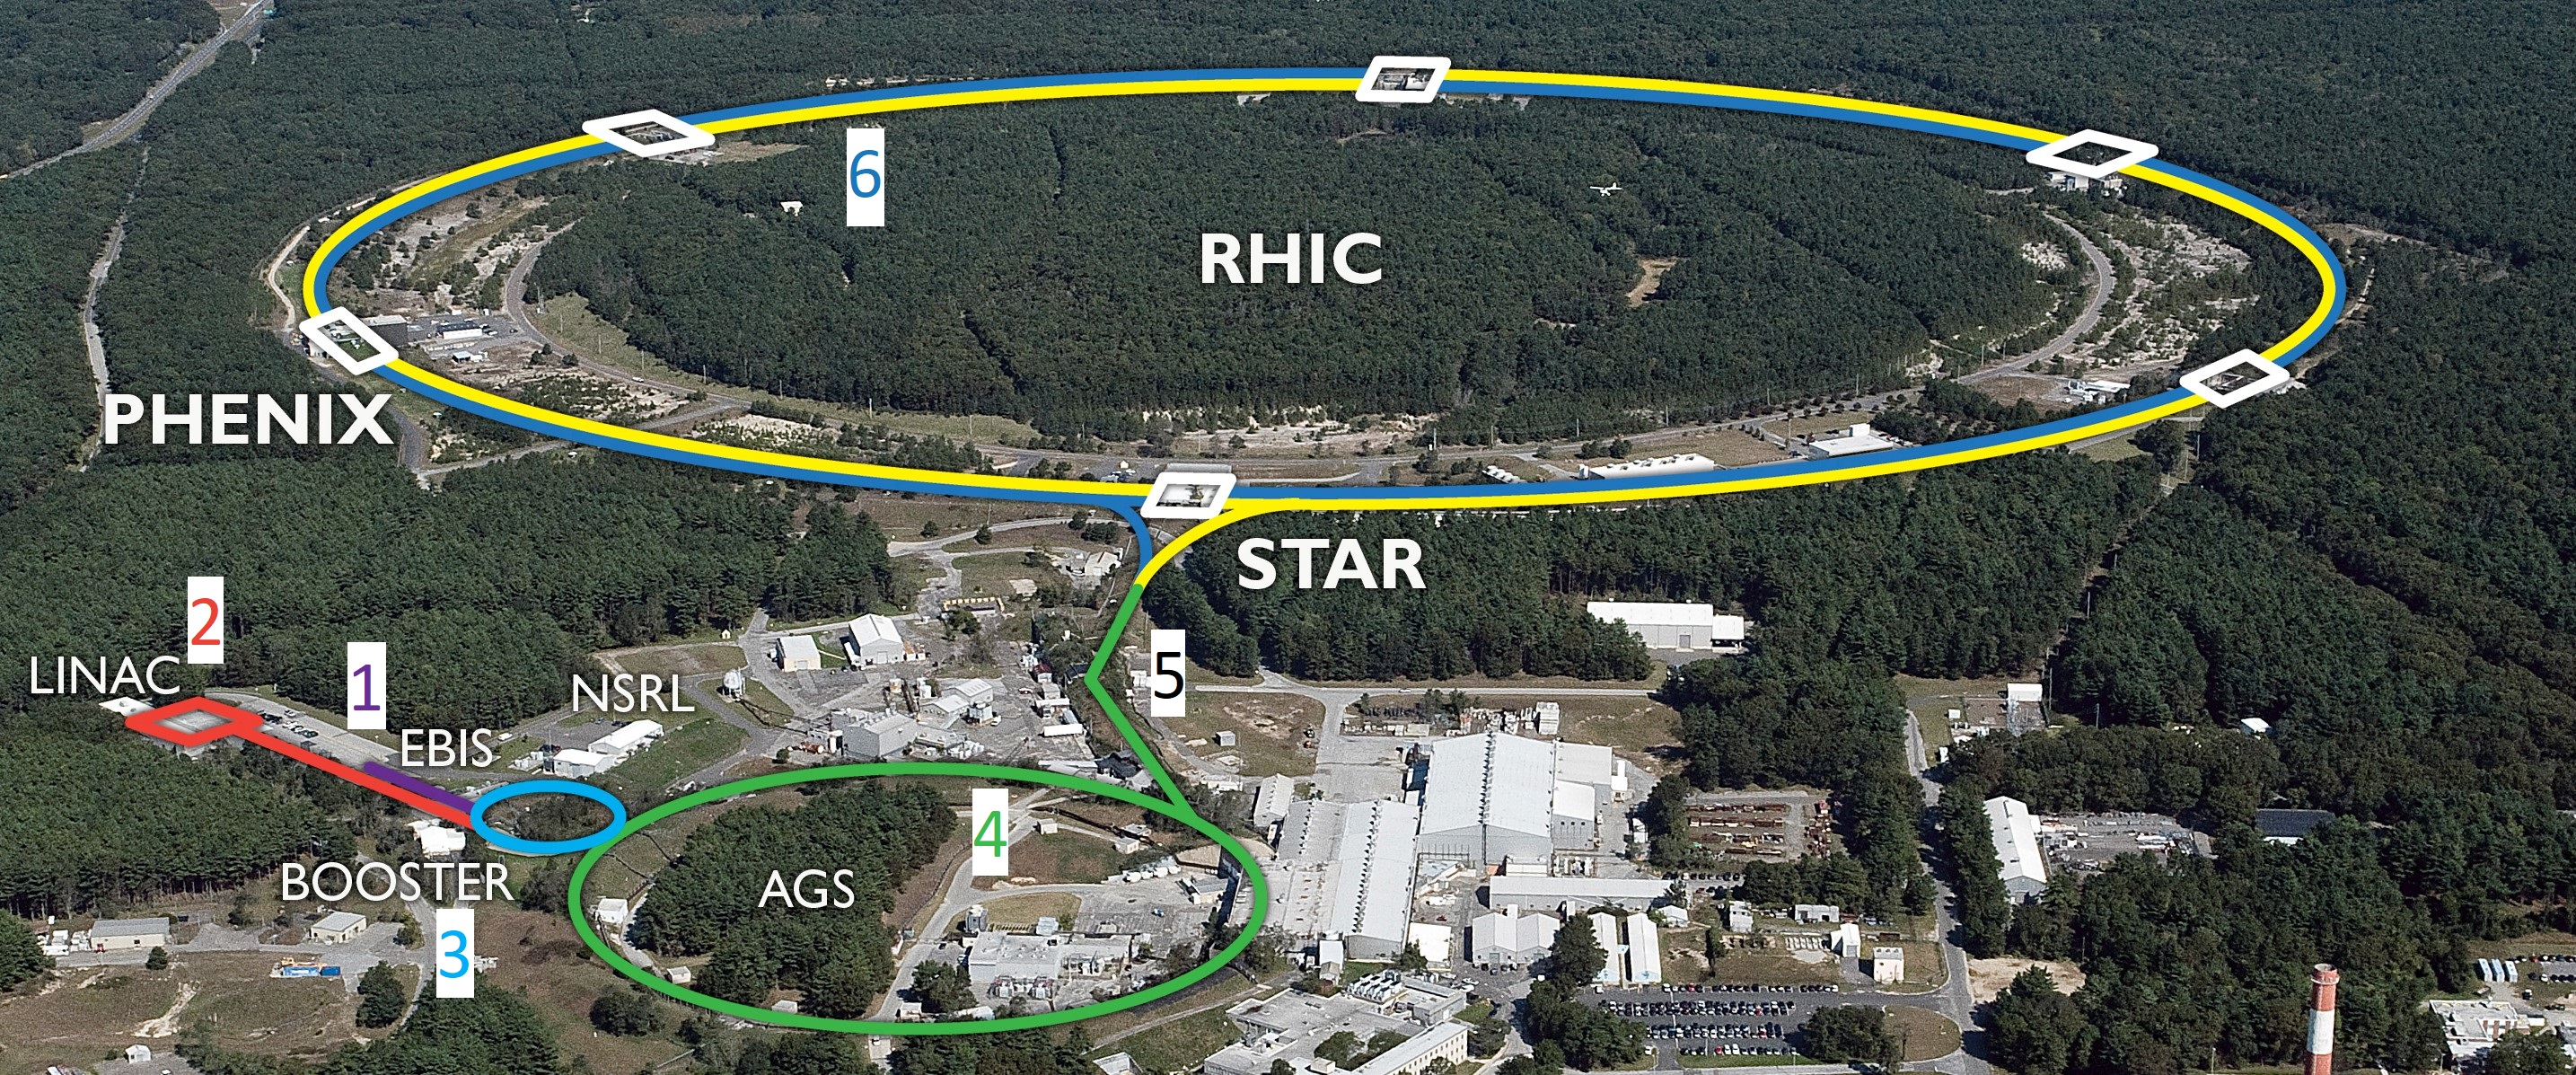
\includegraphics[scale=0.5]{Accelerating_System/written}
	\caption{Εικόνα του επιταχυντικού Συστήμαος στο BNL [1] Electron Beam Ion Source, [2] Linax, [3] Booster Synchrotron, [4] Alternating Gradient Synchrotron, [5] ACS to RHIC Line, [6] RHIC}
\end{figure}

	\section{Η Πορεία των Βαρέων Ιόντων}
	Ένα από τα πειράματα στον RHIC είναι η σύγκρουση δεσμών βαρέων ιόντων, στην αρχή της λειτουργίας του κυρίως Χρυσού, ενώ έπειτα από μία αναβάθμιση του συστήματος δημιουργίας των ιόντων είναι εφικτή και η σύγκρουση βαρύτερων ιόντων όπως Ουρανίου. Μετά την δημιουργία τους, προκειμένου να τους δώσουμε τα επιθυμητά χαρακτηριστικά, τις εισάγουμε διαδοχικά σε τρεις επιταχυντές πρωτού φτάσουν τελικά στον RHIC. Ο κάθε ένας από αυτούς πραγματοποιεί μία διαφορετική επεξεργασία της δέσμης.
	
	\subsection{Electron Beam Ion Source (EBIS)}
	Στις αρχές της λειτουργίας του πειράματος, από το 2000 έως το 2010, η πηγή των ιόντων ήταν ένα σύστημα που λέγεται Tandem Van de Graaff (TVGD). Πρόκειται για δύο διαδοχικούς και ανεξάρτητους επιταχυντές TVGD που μπορούσαν να επιταχύνουν ιόντα προερχόμενα από διαφορετικές πηγές. 
	Ωστόσο, επειδή αυτοί οι επιταχυντές ήταν παλιάς τεχνολογίας έθεταν περιορισμούς ως προς την δυνατότητα δημιουργίας δέσμης από διαφορετικά ιόντα και η αρχή λειτουργίας τους επίτασσε η αρχική πηγή να παρέχει μόνο ανιόντα. Υπήρχαν δύο περιοχές, η πρώτη με διαφορά δυναμικού +V ενώ η δεύτερη με –V. 
	Έτσι αναγκαστικά έπρεπε να ξεκινήσουν με ανιόντα, να τα επιταχύνουν στην πρώτη περιοχή, έπειτα στην μεση των δύο περιοχών να τοποθετήσουν ένα υλικό το οποίο θα απομάκρυνε δύο ηλεκτρόνια έτσι ώστε να δημιουργήσουν τα επιθυμητά κατιόντα τα οποία θα επιταχύνονταν στην δεύτερη περιοχή.
	
	Ήταν λοιπόν αναγκαία η αντικατάσταση του εν λόγω συστήματος για την αρχική δημιουργία και επιτάχυνση των ιόντων  και το 2010 ξεκίνησε την λειτουργία του το σύστημα Electron Beam Ion Source (EBIS). Το EBIS έχει την δυνατότητα να ξεκινάει την λειτουργία του όχι μόνο με ανιόντα, αλλά ακόμη με κατιόντα και ουδέτερα άτομα και επιπλέον μπορεί να εναλλάσσει τις δέσμες που επιταχύνει μέσα σε ένα δευτερόλεπτο. Δηλαδή, αν προετοιμάζει μία δέσμη με κατιόντα χρυσού για τον RHIC, μόλις ένα δευτερόλεπτο μετά μπορεί να προετοιμάσει μία δέσμη από διαφορετικό στοιχείο για άλλες ανάγκες του BNL. 
	
	Τo EBIS απότελείται από έναν θάλαμο 1.5m ο οποίος περικλείεται από έναν κυκλινδρικό υπεραγώγιμο μαγνήτη. Έτσι δημιουργείται στο εσωτερικό του θαλάμου μία μαγνητική παγίδα στην οποία  είναι εγκλωβισμένα τα ιόντα που εισάγονται από εξωτερική πηγή. Στην μία άκρη του θαλάμου υπάρχει ένα Electron Gun που εκπέμπει ηλεκτρόνια 10Α μέσω θερμιονικής εκπομπής, ενώ στην άλλη υπάρχει ένας συλλέκτης ηλεκτρονίων. 
	Καθώς εισάγονται τα ιόντα που θέλουμε να δημιουργήσουμε εισάγονται παγίδα ως αερίο ουδέτερων ατόμων ή ιονισμένων με $1^+$, περνάει από την ίδια περιοχή η δέσμη ηλεκτρονίων. 
	Η δέσμη ιονίζει περεταίρω τα ιόντα τα οποία μπορούν να εξαχθούν οποιαδήποτε στιγμή έχουν αποκτήσει το απαιτούμενο φορτίο. Για την χρήση στον RHIC, χρησιμοποιείται συχνά χρυσός ο οποίος παραμένει στην παγίδα έως ότου γίνει $ Au^{+32}$.% To +32 έχει να κάνει με τις προδιαγραφές των επόμενων προ-επιταχυντών μέσω των οποίων περνά πριν καταλήξει στον RHIC.
	
	Στο τέλος θαλάμου υπάρχει ένας ηλεκτροστατικός φακός ο οποίος χρησιμεύει στην διεύρυνσης της δέσμης κατά την εισαγωγή της στην παγίδα και για την εστίαση κατά την εξαγωγή της. Αφού εξαχθεί, η δέσμη οδηγείται σε δύο αρχικούς γραμμικούς προεπιταχυντές. Ο πρώτος είναι ένας Radio-Frequency Quadrupole (RFQ Linac), ο οποίος είναι ένας κυλινδρικός κυματοδηγός με τέσσερα ηλεκτρόδια τοποθετημένα σε σχήμα σταυρού, όπως φαίνεται στην Εικόνα (\ref{fig2.2}). Στο εσωτερικό του, δεδομένου ότι υπάρχουν συνθήκες κενού, από την κυματική εξίσωση  $\Box^2 \textbf{E}=0$ με συνοριακές συνθήκες $\textbf{E}_\parallel =0 \& \textbf{B}_\perp = 0$ μπορούν να δημιουργηθούν Transverse Electric Modes ($TE_{nlm}$) και Transverse Magnetic Mοdes ($TM_{nlm}$). Επειδή η κοιλότητα έχει τα τέσσερα ηλεκτρόδια, μπορούμε να επιβάλλουμε τον $TE_{210}$ καθώς αυτός είναι βολικός για τον περιορισμό της δέσμης και την διατήρηση της εστίασής της.
	
	Πιο συγκεκριμένα, θεωρούμε πως η δέσμη θετικών ιόντων εισέρχεται στον RFQ με ακριβώς κυκλικό σχήμα, ταχύτητα β και πως το ΗΜ κύμα έχει συχνότητα f. Επειδή οι πολικότητες στα τέσσερα ηλεκτρόδια είναι εναλλάξ, η δέσμη θα συμπιεστεί στην κατεύθυνση των θετικών ηλεκτροδίων ενώ θα αποσυμπιεστεί στην κατεύθυνση των αρνητικών δημιουργώντας μία έλλειψη (Εικόνα \ref{fig2.2}). Έπειτα από μισή περίοδο, οι παραπάνω δυνάμεις αλλάζουν πρόσημο οδηγώντας την σε συμπίεση/αποσυμπίεση κατά τους αντίθετους άξονες. 
	Μέχρι στιγμής δεν έχουμε καταφέρει κάτι ως προς την επιτάχυνση της δέσμης. Το μόνο που συμβαίνει είναι ότι η δέσμη να ταξιδεύει εντός ενός κυματοδηγού, παρουσία Η/Μ πεδίου που προέρχεται από στάσιμα ραδιοκύματα με αποτέλεσμα την εστίασή της εξαιτίας της γεωμετρίας του κυματοδηγού. Τώρα, αν μεταβάλλουμε την απόσταση των απέναντι ηλεκτροδίων με περιοδικό τρόπο ως προς τον χώρο (π.χ. ημιτονοειδώς) , με περίοδο $\beta\lambda/2$, δημιουργούνται και διαμήκεις συνιστώσες ΗΜ πεδίου που επιταχύνουν τα σωματίδια της δέσμης (Εικόνα (\ref{fig2.3})).
	
	
	\begin{figure}[h!]
\centering
\begin{minipage}[c]{0.5\textwidth}
  \centering
  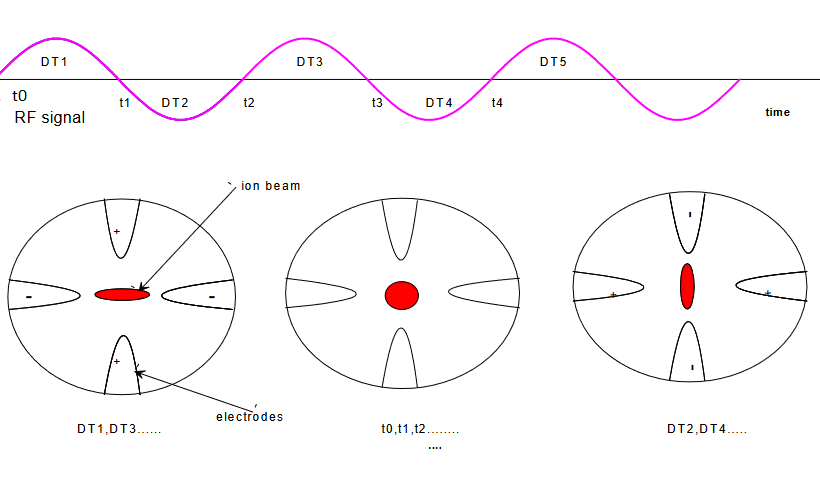
\includegraphics[width=1.1\linewidth]{Accelerating_System/quadtrupole.png}
  \caption{Τομή του κυματοδηγού στον RFQ}
  \label{fig2.2}
\end{minipage}\hfill
\begin{minipage}[r]{0.5\textwidth}\hfill
	\centering
	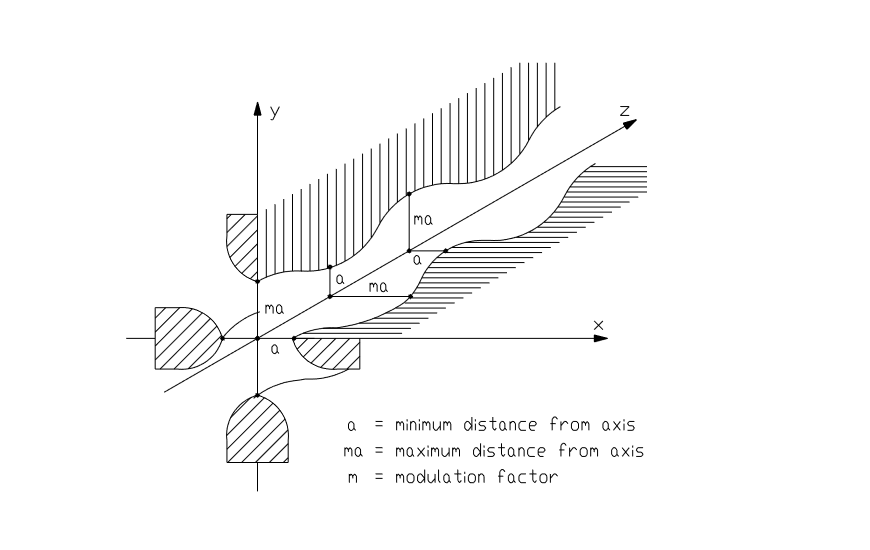
\includegraphics[width=1.3\linewidth]{Accelerating_System/long_modulation_of_wave_guide_in_RFQ.png}
	\caption{Διαμήκης περιοδική μεταβολή του κυματοδηγού για την επιτάχυνση της δέσμης}
	\label{fig2.3}
\end{minipage}
\end{figure}

%	\begin{figure}[!tbp]
%  \centering
%  \subfloat[][Συμπεριφορά του ΤΕ εντός της κοιλότητας]{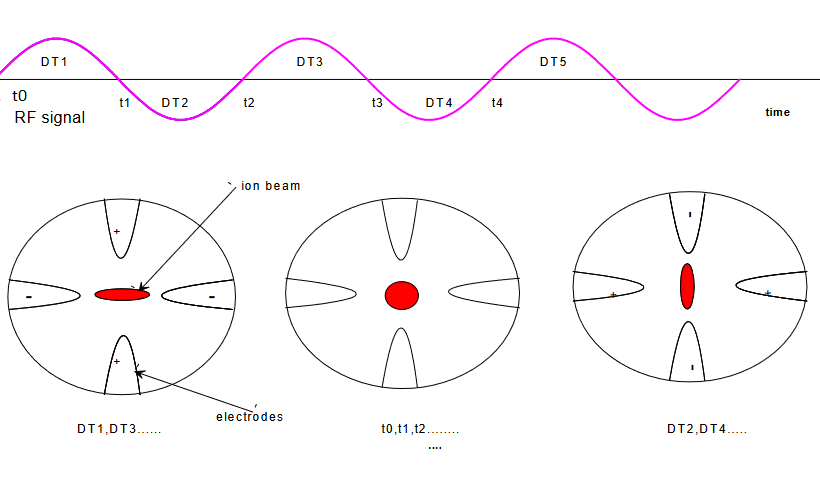
\includegraphics[width=0.5\textwidth]{Accelerating_System/quadtrupole.png}\label{fig:f1}}
%  \hfill
%  \subfloat[][Χωρική μεταβολή του RFQ]{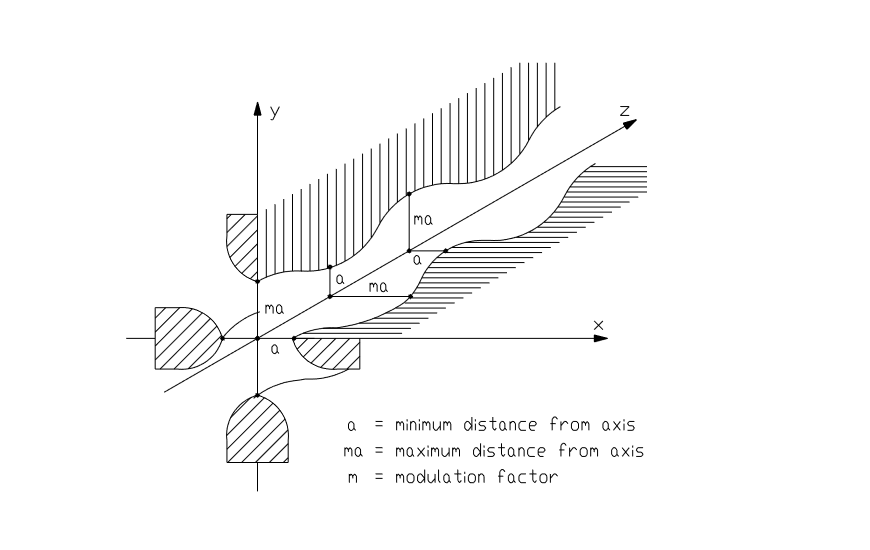
\includegraphics[width=0.5\textwidth]{Accelerating_System/long_modulation_of_wave_guide_in_RFQ.png}\label{fig:f2}}
%  \end{figure}


%\begin{figure}[!h] 
%	\centering 
%	\begin{minipage}[t]{4cm} 
%		\centering 
%		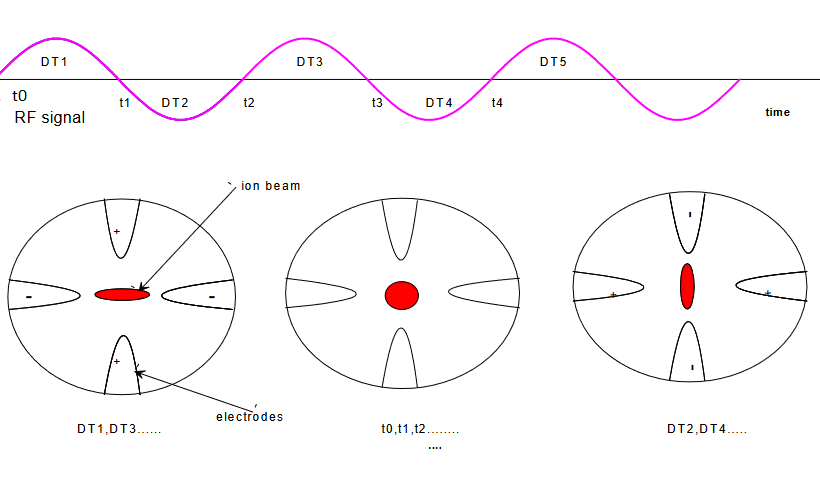
\includegraphics[scale=0.8]{Accelerating_System/quadtrupole.png} 
%		\caption{Caméra thermique 1} 
%	\end{minipage} 
%	\hspace{3cm} 
%	\begin{minipage}[t]{4cm} 
%		\centering 
%		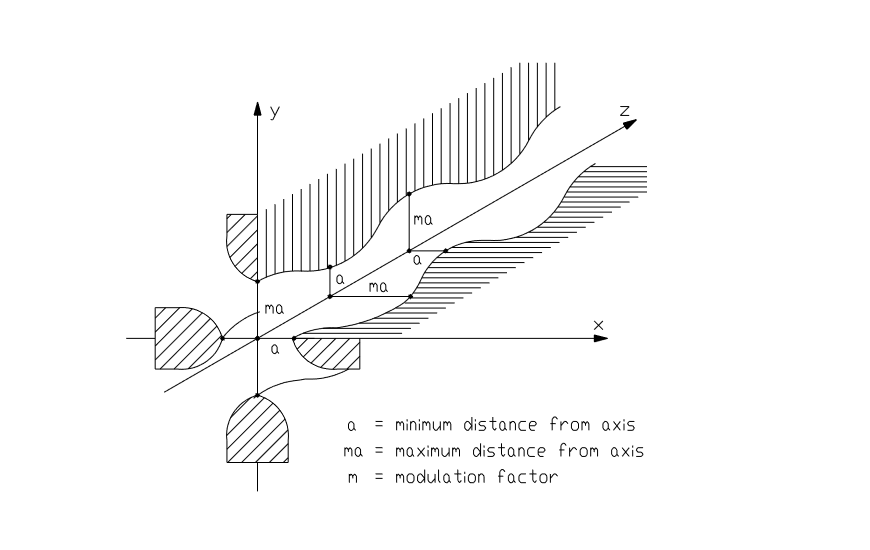
\includegraphics[scale=0.8]{Accelerating_System/long_modulation_of_wave_guide_in_RFQ.png} 
%		\caption{Caméra thermique 2} 
%	\end{minipage} 
%\end{figure} 



	
	Κατά την εξαγωγή της δέσμης από τον RFQ, εισάγεται σε έναν γραμμικό επιταχυντή IH-Linac (Interdigital H-Linear Accelerator). Ο επιταχυντής αποτελείται από μία κοιλότητα στην οποία είναι τοποθετημένοι διακριτοί ομοαξονικοί σωλήνες στο ενδιάμεσο των οποίων υπάρχει κενός χώρος. Ακόμη, σε όλον αυτόν τον χώρο υπάρχει ηλεκτρικό πεδίο που προέρχεται από ραδιοκύματα συχνότητας $f_{RF}$. 
	%Ο επιταχυντής αποτελείται από μία κοιλότητα στην οποία υπάρχει ηλεκτρικό πεδίο που προέρχεται από ραδιοκύματα. 
	
	
	Συνεπώς, η ηλεκτρική συνιστώσα της δύναμης που δέχεται το κάθε σωματίδιο της δέσμης είναι 
	\begin{equation}\label{eq1}
		\bm{F_E} = q \bm{E} = q \bm{E_0}e^{i\omega t}cos(ks),  q>0 
	\end{equation}
	Άρα η ώθηση που κερδίζει δίνεται από την ολοκλήρωση του $2^{ου}$ νόμου του Newton
	\begin{align*}\label{eq2}
		\odv{mc\gamma\bm{\beta}}{t} = q \bm{E} \Rightarrow \\
		\Delta p = m(\gamma\bm{\beta}-\gamma_0\bm{\beta_0}) = q \int\bm{E}dt \numberthis
	\end{align*}
	
	Συνεπώς όταν το ηλεκτρικό πεδίο παίρνει αρνητικές τιμές, η ώθηση θα είναι αρνητική και τα σωματίδια θα χάνουν ορμή. Για αν αποφύγουμε το παραπάνω πρόβλημα μπορούμε να τοποθετήσουμε στο εσωτερικό της κοιλότητας ομοαξονικούς σωλήνες μεταξύ των οποίων θα υπάρχει κενός χώρος. Οι σωλήνες θα είναι έτσι τοποθετημένοι ώστε όταν το πεδίο, άρα η ώθηση γίνεται αρνητική τα σωματίδια να περνάνε από το εσωτερικό του. 
	Τότε, αυτοί θα δρουν ως κλωβοί Faraday και θα θωρακίζουν την δέσμη από το πεδίο στο εξωτερικό τους το οποίο θα την επιβράδυνε. Ταυτόχρονα δεν αλλοιώνουν σημαντικά τους κάθετους ρυθμούς του πεδίου στον ενδιάμεσο χώρο. 
	Επομένως, εμείς θέλουμε τα σωματίδιά μας να εισέλθουν στον χώρο εκτός των σωλήνων όταν το πεδίο θα γίνεται επιταχυντικό, δηλαδή για διάστημα $\Delta t_{RF}=1/2f_{RF}$   σε κάθε περίοδο. Για να έχουμε την βέλτιστη επιτάχυνση, θα πρέπει η αλληλεπίδραση σωματιδίου-κύματος να ξεκινάει για ίδια φάση του κύματος. 
	Έτσι η επιτάχυνση κάθε περιοχή θα είναι ίδια και στο πέρας της j-οστής περιοχής θα είναι απλώς $j\cdot\alpha_1$.  Αυτή η φάση που πρέπει να έχει το κύμα καλείται synchronous phase και συμβολίζεται $\psi_s$. Άρα θα πρέπει να ισχύουν: 
	\begin{align*}\label{eq3}
		\psi_s         =& \omega t_j - kz_j   = const.\Rightarrow\\
		\odv{\psi_s}{t}=& \omega - k\beta_jc  = 0 \numberthis
	\end{align*}
	
	Ο χρόνος που μένουν τα σωματίδια εντός και εκτός των επιταχυντικών περιοχών είναι μισή περίοδος, άρα η διαφορά φάσης που βλέπουν στις δύο περιοχές εισόδου-εξόδου είναι $\pi$.
	
  Δεν θα πρέπει να αμελήσουμε το γεγονός ότι η απόσταση που διανύει η δέσμη σε αυτόν τον χρόνο αυξάνεται καθώς αυτή κινείται εντός του επιταχυντή. Όταν έχει περάσει από την j-οστή περιοχή επιτάχυνσης θα έχει ταχύτητα $u_i$ και η απόσταση που θα διανύει σε $1/2f_{RF}$ είναι 
	\begin{align}\label{eq4}
		l_i = \frac{u_i}{2f_{RF}} = \frac{u_i\lambda_{RF}}{2c} = \frac{\beta_i\lambda_{RF}}{2}
	\end{align}
	
	Η ενέργεια που κερδίζει με κάθε διέλευση από την j-oστή περιοχή επιτάχυνσης μήκους $l_j$ είναι
		\begin{align}\label{eq5}
			\Delta E_{kin} =q \int_{r_j}^{r_{j+1}}\bm{E}\cdot d\bm{s} = q E_{0s}e^{i(\omega t_j+\pi)} \left(-\frac{sink_jl_j}{k_j}-0\right) = \frac{qE_{0s}e^{i\omega t_j}sink_jl_j}{k_j}
		\end{align}
		
		Άρα αν θεωρήσουμε ως $T_0$ την κινητική ενέργεια με την οποία εισέρχεται στον IH-Linac, από την συνολική κινητική ενέργεια στην j επιταχυντική περιοχή και στο μη σχετικιστικό όριο προκύπτει και η ταχύτητα που θα έχει η δέσμη 
			\begin{align*}\label{eq6}
					T_j       =& T_0 + j\Delta E_{kin} = m(\gamma -1)c^2 \xRightarrow{non relat. limit} \\ 
					\beta_j^2 =& \frac{u_j^2}{c^2} = \frac{2(T_0 +j\Delta E_{kin})}{mc^2}  \numberthis
			\end{align*}
			
			Συνεπώς από τις σχέσεις (\ref{eq3}), (\ref{eq6}) έχουμε ότι το μήκος των σωλήνων θα αυξάνεται $\sim\sqrt{j}$. Ακόμη, δεν θα πρέπει να χρησιομποιήσουμε $\psi_s=\pi/2$ που αντιστοιχεί στο μέγιστο του πεδίου άρα στο μέγιστο της δύναμης που δέχονται τα σωματίδια. 
			Αυτό διότι όταν έχουμε μεγάλο αριθμό j σταδίων επιτάχυνσης τότε η ταχύτητα των σωματιδίων θα αποκλίνει από την θεωρητικά σχεδιασμένη, επομένως τα σωματίδια θα βλέπουν διαφορετική φάση του κύματος καθώς εισέρχονται στην περιοχή επιτάχυνσης και ο συγχρονισμός κύματος-σωματιδίου θα χάνεται. 
			Ωστόσο αν χρησιμοποιήσουμε $\psi_s<\pi/2$, τότε παρ'ολο που δεν έχουμε την μέγιστη επιτάχυνση, αν η ταχύτητα αρχίσει να αποκλίνει έπειτα από κάποια στάδια, τα σωματίδια θα βλέπουν το κύμα σε διαφορετική φάση $\psi_s\pm\Delta\psi$, ανάλογα με το αν έχουν επιταχυνθεί περισσότερο ή λιγότερο από το αναμενόμενο. Έτσι, αν για παράδειγμα κάποιο έχει μεγαλύτερη ταχύτητα από την αναμενόμενη, θα βλέπει το κύμα σε μικρότερη φάση $\psi_s-\Delta\psi$, άρα σε μικρότερη τιμή του πεδίου του με αποτέλεσμα να επιταχύνεται λιγότερο από όσα έχουν επιταχυνθεί λιγότερο από το επιθυμητό. Όσα έχουν επιταχυνθεί λιγότερο, θα βλέπουν το κύμα σε μεγαλύτερη φάση, άρα μεγαλύτερο πεδίο.
			
			
			Κατ’ αυτόν τον τρόπο, επιτυγχάνεται ένα κλείδωμα φάσης που οδηγεί σε σχεδόν ομοιόμορφη επιτάχυνση όλων των σωματιδίων της δέσμης. Φυσικά, οι εξισώσεις και οι υπολογισμοί σε έναν πραγματικό HI-Linac είναι πιο πολύπλοκες από τις παραπάνω καθώς θα πρέπει να λάβουμε υπ΄όψιν και άλλες παραμέτρους.%
%			, όπως η αλλοίωση του πεδίου από την τοποθέτηση των σωλήνων.
			 Ένα σχήμα HI-Linac φαίνεται στην Εικόνα (\ref{fig2.4}).
			
			\begin{figure}[h!]
				\centering
				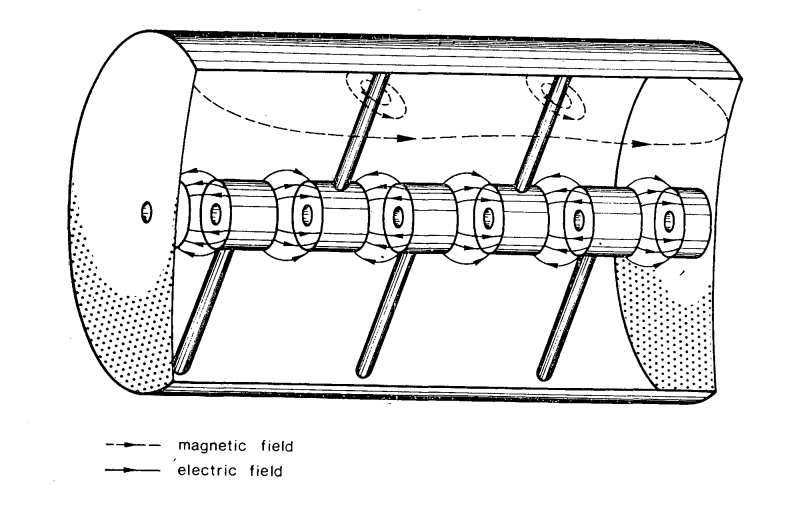
\includegraphics[scale=0.5]{linac.png}
				\caption{Σχέδιο HI-Linac}
				\label{fig2.4}
			\end{figure}
			
			
			
			
			
			
			
			
\subsection{Booster Synchrotron}

Η δέσμη των βαρέων ίοντων, εξέρχεται από το σύστημα EBIS-RFQ-HI Linac όχι σε συνεχή μορφή αλλά παλμικά, και οδηγείται στον επόμενο προεπιταχυντή, τον Booster Synchrotron (Εικόνα (\ref{fig2.5})) μέσω του Beam Port. Για τον RHIC εισέρχονται στον Booster Synchrotron $^3He^{2+}, ^4He^{1+}, ^4He^{2+}$, $ Cu^{11+}, Au^{32+}, U^{39}$ με ενέργεια έως 2MeV/n. 

	\begin{figure}[h!]
		\centering
		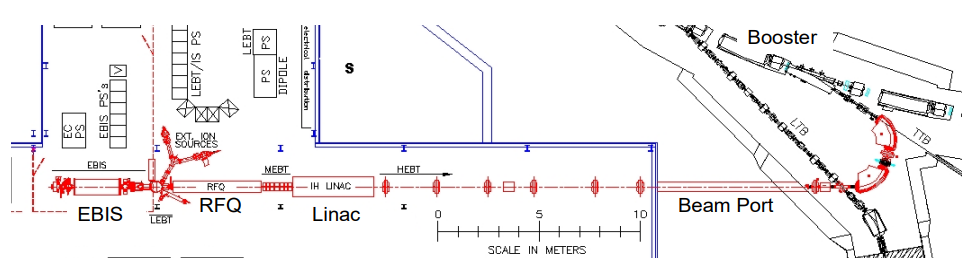
\includegraphics[scale=0.5]{Accelerating_System/1st_stage.png}
		\caption{1ο στάδιο επιτάχυνσης}
		\label{fig2.5}
	\end{figure}
	
	Πριν την ολοκλήρωση της κατασκευής του το 1990, όταν ακόμη ο κύριος επιταχυντής ήταν ο AGS και όχι ο RHIC,\footnote{Πλέον o AGS λειτουργεί ως προεπιταχυντής για τον RHIC} δεν ήταν δυνατή η επιτάχυνση όλων των ιόντων στον AGS. 
	Επειδή ο AGS μπορεί να επιταχύνει σχεδόν πλήρως ιονισμένα άτομα, θα έπρεπε να τα έχουμε ιονίσει πρωτού τα εισάγουμε σε αυτόν, επομένως
	%και ο εν λόγω ιονισμός στο πρόγραμμα βαρέων ιόντων του AGS εκείνης της εποχής ήταν αδύνατος για άτομα βαρύτερα του Θείου.
	ο ρόλος του Booster Synchrotron είναι να προεπιταχύνει τα ιόντα και ταυτόχρονα να τα ιονίσει περεταίρω ώστε να μπορούν να επιταχυνθούν επιτυχώς στον AGS. Πέρα από τα ιόντα, έχει σημαντικό ρόλο και στην προεπιτάχυνση των πρωτονίων όπως θα δούμε στην συνέχεια.
	
	Έχει περιφέρεια 207.78m, το 1/4 της περιφέρειας του AGS και όντας σύγχροτρο αποτελείται από ένα πλέγμα κυψελίδων εντός των οποίων η ταχύτητα της δέσμης αλλάζει κατεύθυνση και μέτρο.
	 Τα κελιά που έχουν χρησιμοποιηθεί είναι τύπου FODO (\textbf{F}ocusing - Χώρος Ολίσθησης \textbf{O} - \textbf{D}efocusing - \textbf{O}), αποτελούνται δηλαδή από δύο τετραπολικούς μαγνήτες με αντίθετες πολικότητες οι οποίοι εστιάζουν την δέσμη σε διαφορετικές κατευθύνσεις. Ενδιάμεσα από αυτούς τους μαγνήτες καθώς και στο τέλος της κεψελίδας υπάρχει ένα διπολικός μαγνήτης ο οποίος χρησιμεύει για να στρίψει την δέσμη. Στον συγκεκριμένο επιταχυντή λείπει ο πρώτος διπολικός από κάθε δεύτερο κελί.
	 Συνολικά έχει 6 συστοιχείες εκ των οποίων η κάθε μία 4 FODO κυψιλίδες 
	Η μέγιστη ενέργεια με την οποία εξάγονται τα βαρέα ιόνται από τον Booster Synchrotron ποικίλλει από 0.35-1GeV ανάλογα το ιόν
\subsection{Alternating Gradient Synchrotron (AGS)}


	Το AGS κατασκευάστηκετο 1960 και για τα επόμενα οκτώ χρόνια ήταν ο επιταχυντής με την υψηλότερη ενέργεια, επιταχύνοντας αρχικά πρωτόνια στα 33GeV και έπειτα ιόντα με μία ενδεικτή ενέργεια για τον χρυσό στα 14.5GeV/n.
	Το συνολικό μήκος της περιφέρειάς του είναι 842.90m και αποτελείται από 240 μαγνήτες. Οι δέσμες εισάγονται στον AGS σε 24 bunches τα οποιά γίνονται μία δέσμη και εν τέλει ξαναχωρίζονται σε 4 για να οδηγηθούν στον RHIC.
	
	 Είναι ο πρώτος επιταχυντής που χρησιμοποίησε την αρχή της Ισχυρής Εστίασης (Strong Focusing/Alternating Gradient Focusing Principle) την οποία σκέφτηκε για πρώτη φορά ο Ν. Χριστόφιλου το 1949 και έπειτα, το 1952 ανακαλύφθηκε ανεξάρτητα από τρεις επιστήμονες του BNL. 
	 Η εν λόγω αρχή είναι αυτή που χρησιμοποιείται και στον Booster Synchrotron και σύμφωνα με αυτή, αν τοποθετήσουμε διαδοχικά τετραπολικούς μαγνήτες αντίθετης πολικότητας, εκ των οποίον ο ένας εστιάζει και ο άλλος διευρύνει την δέσμη, το τελικό αποτέλεσμα θα είναι η εστίασή της και ταυτόχρονα η μείωση του μεγέθος των μαγνητών που ελαττώνει σημαντικά το κόστος κατασκευής. 
	
	Το κάθε κελί του AGS είναι της μορφής FOFDOD και πέρα από αυτά, αποτελείται επίσης από 24 ευθύγραμμα τμήματα μήκους 3.15m. Το μαγνητικό πεδίο που καμπυλώνει την δέσμη πρέπει να είναι μικρότερο όταν αυτή εισάγεται στον επιταχυντή έχοντας μικρή ενέργεια και μεγαλύτερο όταν εξάγεται προς τον RHIC. Αυτό μπορεί να εξηγηθεί πρόχειρα από τον 2ο νόμο του Newton από τον οποίο προκύπτει για την ακτίνα ότι $1/R = ecB_\perp/cp$. Αυτό σημαίνει πως για να διατηρηθεί η ακτίνα σταθερή θα πρέπει καθώς αυξάνεται η ενέργεια άρα και η ορμή του σωματιδίου, να αυξάνεται και το μαγνητικό πεδίο που στρίβει το σωματίδιο.
	
	Τα πρώτα σύγχροτρα ήταν ακριβώς κυκλικά μέχρι που κατασκευάστηκαν τα Bevatron και Cosmotron τα οποία είχαν και ευθύγραμμα τμήματα μεταξύ των μαγνητών, διότι εν γένει είναι ευκολότερη η συγκράτηση, η επιτάχυνση και η διατήρηση των χαρακτηρηστικών της δέσμης όταν υπάρχουν ευθύγραμμα τμήματα επιτάχυνσης.
	Ωστόσο, αν αυξηθούν αρκετά τα εν λόγω τμήματα δημιουργούνται ορισμένα προβλήματα με το σημαντικότερο να είναι πως θεωρητικά, την εποχή κατασκευής του AGS περίμεναν μία ασταθεια στην δέσμη για μία συγκεκριμένη τιμή της ενέργειας (transition energy) η οποία βέβαια εξαφανίζεται για μικρότερες και μεγαλύτερες τιμές ενεργειών. 
	Αυτή η αστάθεια προβλημάτιζε τους επιστήμονες που σχεδίαζαν το AGS και παρ'όλο που θεωρητικά προβλεπόταν πως η μετάβαση από αυτή ήταν πολύ γρήγορη, τους οδήγησε στο να την ελέγξουν με ένα μικρότερο σύγχροτρο ηλεκτρονίων της τάξης MeV. Αφού επιβεβαίωσαν την θεωρητική πρόβλεψη συνέχισαν με την κατασκευή του AGS. Στα επόμενα 30 χρόνια λειτουργίας του προέκυψαν από το AGS τρία βραβεία Νόμπελ, σχετιζόμενα με την παραβίαση της CP συμμετρίας, την ανακάλυψη του μιονικού νετρίου και του σωματιδίου J/$\psi$.
\subsection{Relativistic Heavy Ion Collider}

Πλέον ο AGS έχει πολύ μικρή ενέργεια και δεν μπορεί να συγκριθεί με τους σύγχρονους επιταχυντές. Ωστόσο, αυτό για το οποίο είναι χρήσιμος είναι το να προεπιταχύνει τις δέσμες ιόντων και πρωτονίων για τον RHIC (Εικόνα (\ref{fig2.6})). Η μεταφορά γίνεται μέσω μίας γραμμής \textit{AGS-to-RHIC Line}, στην αρχή της οποίας ο χρυσός από +77 ιονίζεται πλήρως σε +79 και στο τέλος της οι δέσμες χωρίζονται στα δύο δαχτυλίδια του RHIC, που απέχουν 90cm, με αντίθετη φορά περιστροφής.
	Η μέγιστη ενέργεια για τις συγκρούσεις ιόντων Χρυσού είναι 100GeV/n οι οποίες πραγματοποιούνται σε 6 σημεία αλληλεπίδρασης (Interaction Points - IP) και το αποτέλεσμά τους είναι η δημιουργία τόσο υψηλών θερμοκρασιών $\sim TerraK$ που εμφανίζεται μία νέα κατάσταση της ύλης στην οποία τα κουάρκ και τα γλουόνια αποδεσμεύονται από τα πρωτόνια και τα νετρόνια δημιουργώντας πλάσμα κουάρκ-γλουονίων.
	
	\begin{figure}[h!]
		\centering
		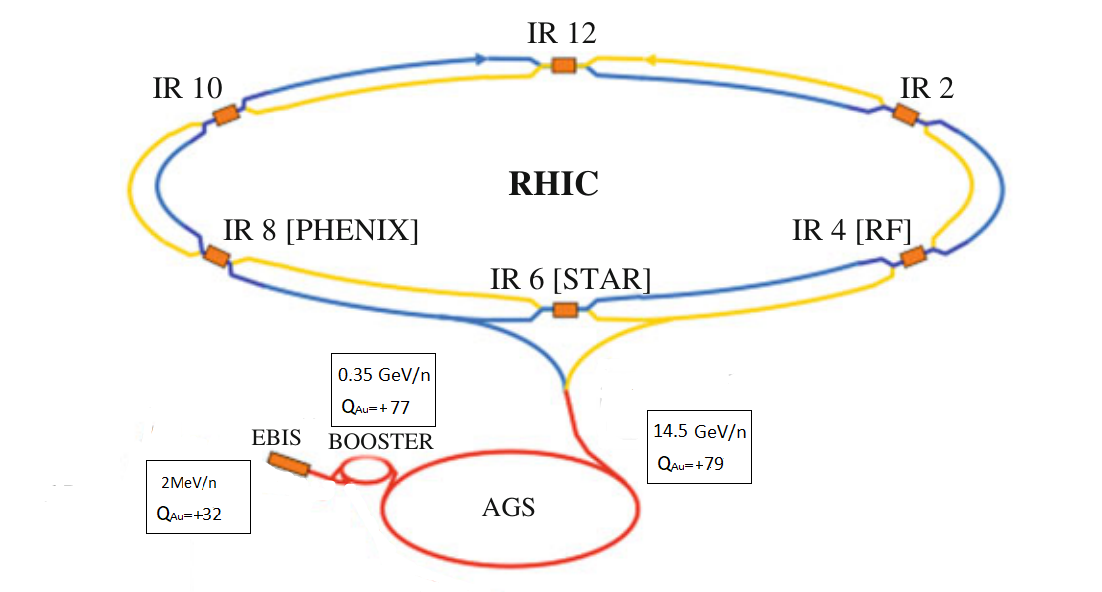
\includegraphics[scale=0.5]{Accelerating_System/RHIC_full.png}
		\caption{Τυπική πορεία των ιόντων με σημειωμένα τις τιμές φορτίου και ενέργειας του Au. }
		\label{fig2.6}
	\end{figure}
		
	
	Ο RHIC αποτελείται από 6 arc-sections μήκους 356m και από 6 insertion-sections μήκους 277m, όπως φαίνεται στην Εικόνα (\ref{fig2.7}). Στο κέντρο των τελευταίων πραγματοποιούνται οι συγκρούσεις. Τα arc-sections αποτελούνται από 11 κυψελίδες τύπου FODO με 2 διπολικούς μαγνήτες που κατευθύνουν την δέσμη, δύο τετραπολικούς οι οποίοι την εστιάζουν και δύο εξαπολικούς που επίσης την εστιάζουν με μεγαλύτερη ακρίβεια και ταυτόχρονα μειώνουν τις χρωματικές αλλοιώσεις που οφείλονται στην διασπορά της ορμής της (Ένα σχέδιο μισής περιόδου του FODO φαίνεται στην Εικόνα (\ref{fig2.8})). Επίσης, κοντά στα IP υπάρχουν επιπλέον μαγνήτες με σκοπό την γρήγορη εστιαση της δέσμης στο σημείο σύγκρουσης.	
	Συνολικά υπάρχουν 1740 υπεραγώγιμοι μαγνήτες με πεδία εως 3.458Τ.
	
	\begin{figure}[h!] 
		\centering
		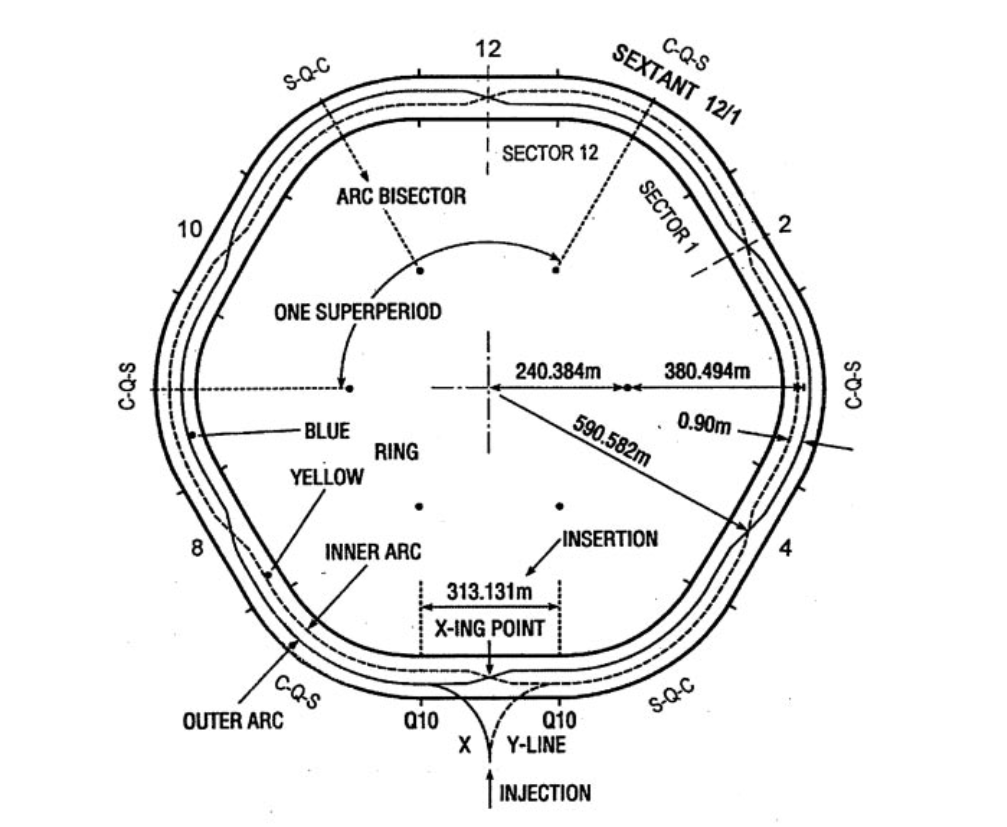
\includegraphics[scale=0.5]{Accelerating_System/RHIC_schem.png}
		\caption{Κάτοψη του RHIC }
		\label{fig2.7}
	\end{figure}
	
	
	Μία τυπική διαδικασία επιτάχυνσης αποτελείται από την εισαγωγή 111 δέσμεων σε ομάδες των 4 σε κάθε ένα από τα δύο δακτυλίδια. Αρχικά, επειδή η ενέργειά τους δεν είναι η μέγιστη,  οι δέσμες στα Interaction Points απέχουν 10mm για να αποφευγχθούν ανεπιθύμητες απώλειες και όταν φτάσουν στην μέγιστη ενέργεια, οι δέσμες συγκρούονται μετωπικά. 
	
	\begin{figure}[h!]
		\centering 
		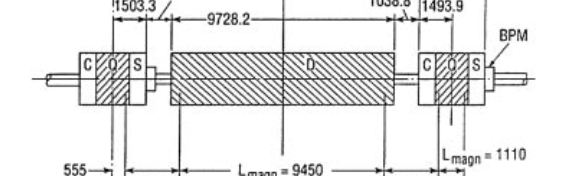
\includegraphics[scale=0.5]{Accelerating_System/RHIC_half_cells.png}
		\caption{ Σχέδιο μισής περιόδου ενός FODO του RHIC}
		\label{fig2.8}
	\end{figure}
	
	
	Όταν φτάσουν σε αυτό το σημείο μέγιστης ενέργειας, τότε ο RHIC λειτουργεί ως Storage Ring. Ο αριθμός των σωματιδίων στην δέσμη είναι πολύ μικρός ($10^9-10^{10}$ ανά bunch) και ως εκτούτου η πιθανότητα αλληλεπίδρασης είναι επίσης μικρή, πόσο μάλλον οι ισχυρές συγκούσεις που απαιτούνται για την δημιουργία των πιό ενδιαφέροντων γεγονότων. Αυτό σημαίνει ότι για να επιτευγχθούν τα απαραίτητα γεγονότα θα πρέπει να διατηρηθεί η δέσμη αρκετές ώρες (έως 10) εντός του RHIC. 
	Ο αριθμός γεγονότων ανά δευτερόλεπτο δίνεται από την σχέση 
		\begin{align*}\label{eq2.7}
			N_p = \sigma_p \mathcal{L} \numberthis
		\end{align*}	
	Όπου $\sigma_p$ είναι η ενεργός διατομή της αλληλεπίδρασης Au-Au και $\mathcal{L}$ είναι η φωτεινότητα της δέσμης. Αυτό σημαίνει πως ο μόνος τρόπος για να αυξήσουμε τον αριθμό αλληλεπιδράσεων, δεδομένου ότι η ενεργός διατομή είναι εγγενές χαρακτηριστικό της εκάστοτε αλληλεπίδρασης, είναι η αύξηση της φωτεινότητας.
		
		Η φωτεινότητα είναι ο λόγος των γεγονότων σε ένα χρονικό διάστημα ανά ενεργό διατομή, δηλαδή ορίζεται από την σχέση $\mathcal{L} = (1/\sigma)dN/dt$ και έχει μονάδες $[cm^{-2}s^{-1}]$. Για έναν collider όπως ο RHIC, υπολογίζεται από την σχέση
			\begin{align}\label{eq2.8}
				\mathcal{L} = \frac{1}{4\pi}\frac{fN_1N_2}{\sigma_x\sigma_y}
			\end{align}
	όπου f συχνότητα περιστροφής των σωματιδίων, $N_1, N_2$ ο αριθμός σωματιδίων σε κάθε δέσμη και $\sigma_x\sigma_y$ η διατομή της δέσμης κάθετα στο επίπεδο κίνησης. Άρα από τα παραπάνω προκύπτει κάτι που είναι και διαισθητικά αναμενόμενο, δηλαδή ότι ο αριθμός των συγκρούσεων αυξάνεται καθώς αυξάνεται η συχνότητα περιστροφής των σωματιδίων, ο αριθμός των σωματιδίων και καθώς εστιάζεται περισσότερο η δέσμη. Στον RHIC η μέση φωτεινότητα είναι $20\times10^{26}cm^{-2}s^{-1}$ για τις συγκρούσεις Au-Au ενώ η μέγιστη δυνατή που επιτυγχάνεται στα IP, σε μία εκ των οποίων  βρίσκεται και το πείραμα STAR, είναι $40\times10^{26}cm^{-2}s^{-1}$
		
		
	
	
	

\section{Η πορεία των πρωτονίων}
	Όπως έχει αναφερθεί, πέρα από τις συγκρούσεις βαρέων ιόντων, το πρόγραμμα του RHIC και των αντίστοιχων ανιχνευτών του περιλαμβάνει και συγκρούσεις πρωτονίων αλλά και πολωμένων πρωτονίων έως και ενέργειες $\sqrt{s} = 500GeV$.
	Κύριοι στόχοι εδώ είναι να μελετηθεί η προέλευση του σπιν των νουκλεονίων, καθώς εκτιμάται ότι τα κουάρκ συνεισφέρουν σε αυτό μόλις κατά ~25\% και επίσης να μελετηθούν ασυμμετρίες στις ενεργές διατομές διαφόρων δεσμών ανάλογα με την πόλωσή τους.
	
	Η δέσμη πολωμένων πρωτονίων ξεκινάει από μία πηγή πολωμένων ιόντων $H^-$.  Η πηγή μπορεί να παράξει ρεύμα 500$\mu A$ σε έναν παλμό διάρκειας $300\mu s$ ο οποίος περιέχει $9\times 10^{11}$ πολωμένα ιόντα $H^-$ σε ποσοστρό 80-85\% καθώς η εν λόγω παραγωγή αποτελείται από πολλά στάδια και σε κάθε ένα από αυτά χάνεται ένα μέρος της πόλωσης. Η τελική ενέργεια είναι 35keV ανά ιόν.
	
	Κατά την έξοδο από την πηγή, τα ιόντα εισέχονται στον γραμμικό επιταχυντή RFQ (Radiofrequenct Quadtrupole), ο οποίος τα επιταχύνει σε ενέργεια 753keV και τα οδηγεί στον LINAC. 
	Ο lINAC πρόκειται για ένα γραμμικό επιταχυντή αποτελεούμενο από κοιλότητες RF και που επιταχύνει τα ιόντα σε ενέργειες 200MeV. Στο τέλος της επιτάχυνσης από τον LINAC, η δέσμη περνάει από μία διαδικασία στην οποία απομακρύνονυαι τα δύο ηλεκτρόνια από το κάθε ιόν και απομένουν τα πολωμένα πρωτόνια που θέλουμε να μελετήσουμε και εν τέλει εισάγονται στον AGS Booster μειωμένα στον μισό πληθυσμό $4\times10^{11}$ ανά παλμό.
	Στον AGS-Booster επιταχύνονται στα 2.4GeV και έπειτα εισάγονται στον AGS ο οποίος τα επιταχύνει στα $24.3GeV$ και τότε οδηγούνται μέσω μίας γραμμής μεταφοράς στον RHIC. 
	Το σημαντικότερο στοιχείο στις επιταχύνσεις πρωτονίων είναι η δημιουργία και η διατήρηση της πόλωσής τους. Για να επιτευγχθεί αυτό χρησιμοποιούνται κάποιοι εξειδεικευμένοι μαγνήτες, οι Siberian Snakes.
	
	
 	Η επιτάχυνση πολωμένων πρωτονίων απαιτεί τον έλεγχο τόσο στην τροχιακή κίνηση, όσο και στην κίνηση του σπιν τους. Ο έλεγχος της τροχιακής τους κίνησης είναι παρόμοιος με αυτόν για τα βαρέα ιόντα, όμως ο έλεγχος του σπιν διαφέρει.
 	
 	
	Η δυναμική του σπιν των πρωτονίων δίνεται από την εξίσωση 
		\begin{align*}\label{eq2.8}
			\odv{\bm{S}}{t} = - \frac{e}{\gamma m}\left( G\gamma \bm{B}_\perp  + (1+G)\bm{B}_\parallel\right) \times\bm{S} \numberthis
		\end{align*}
	
	όπου $\bm{S}$ είναι το διάνυσμα του σπιν σε ένα σύστημα αναφοράς που κινείται μαζί με το σωματίδιο, $\bm{B}_\perp$, $\bm{B}_\parallel$ είναι οι συνιστώσες του μαγνητικού πεδίου κάθετα και παράλληλα στην κατεύθυνση της δέσμης, γ ο παράγοντας Lorentz και G η ανώμαλη μαγνητική ροπή, που για το πρωτόνιο ισούται με $G=1.7928$.
	
	Η σχέση (\ref{eq2.8}), άν δεν περιείχε τον πρώτο όρο, μοίάζει με την εξίσωση για σχετικιστική κίνηση φορτισμένου σωματιδίου σε εξωτερικό μαγνητικό πεδίο 
		\begin{align*}\label{eq2.9}
			\odv{\bm{u}}{t} = - \frac{e}{\gamma m} \bm{B}_\perp \times\bm{u} \numberthis
		\end{align*}
		
Παρατηρούμε πως στην ιδανική περίπτση που το πεδίο είναι μόνο κάθετο στην δέσμη, δηλαδή $\bm{B_\parallel}  = 0$, οι παραπάνω εξισώσεις διαφέρουν μονάχα κατά έναν παράγοντα $G\gamma$. Από αυτά μπορούμε να συμπαιρνάνουμε πως στην ιδανική περίπτωση η μεταπτωτική κίνηση του σπιν γίνεται $G\gamma $ φορές γρηγορότερα από την περιστροφική κίνηση του πρωτονίου.		
	Αυτή την διαφορά στις συχνότητες περιστροφής, την ποσοτικοποιούμε εισάγοντας μία νέα παράμετρο , το \textit{spin tune, }$v_{sp}$. Αυτή είναι μία παράμετρος η οποία ορίζεται ως ο αριθμός των περιστροφών της μεταπτωτικής κίνησης του σπιν σε μία πλήρη κυκλική περιστροφή του σωματιδίου. Στην ιδανική περίπτωση ισχύει ότι $v_{sp}=G\gamma$.\footnote{Στην υψηλότερη ενέργεια του RHIC, $\sqrt{s}=250GeV$ η τιμή της είναι $v_{sp}=476$}	
			
	Η δυσκολία στην επιτάχυνση πολωμένων δεσμών 	έγκειται στους  παράγοντες οι οποίοι καταστρέφουν την πόλωσή τους.
	Ενδεικτικά, ενδέχεται να υπάρχουν μικρά οριζόντια πεδία. Αυτά προκαλούν διαταραχές στο διάνυσμα του σπιν οι οποίες εν τέλει τείνουν να αθροίζονται και να απο-πολώνουν κάποια σωματίδια.
	Ακόμη, υπάρχει και ένας άλλος συντονισμός ο οποίος επιδεινώνει την πόλωση και  εμφανίζεται όταν $v_{sp}=v_{bet}$, όπου $v_{bet}$ το \textit{betatron tune}, δηλαδή ο αριθμός των ταλαντώσεων betatron σε μία πλήρη περιστροφή.
	
%	Για να ποσοτικοποιήσουμε την επίδοση στην διατήρηση της πόλωσης εισάγουμε μία νέα παράμετρο, το \textit{spin tune, }$v_{sp}$. Αυτή είναι μία παράμετρος η οποία ορίζεται ως ο αριθμός των περιστροφών της μεταπτωτικής κίνησης του σπιν σε μία πλήρη κυκλική περιστροφή του σωματιδίου. Στην ιδανική περίπτωση ισχύει ότι $v_{sp}=G\gamma$.
%	Η επιτάχυνση τέτοιων δεσμών γίνεται δύσκολη καθώς υπάρχουν διάφοροι παράγονται οι οποίοι καταστρέφουν την πόλωση. Για παράδειγμα
	
	
	\begin{figure}[h!]
		\centering
		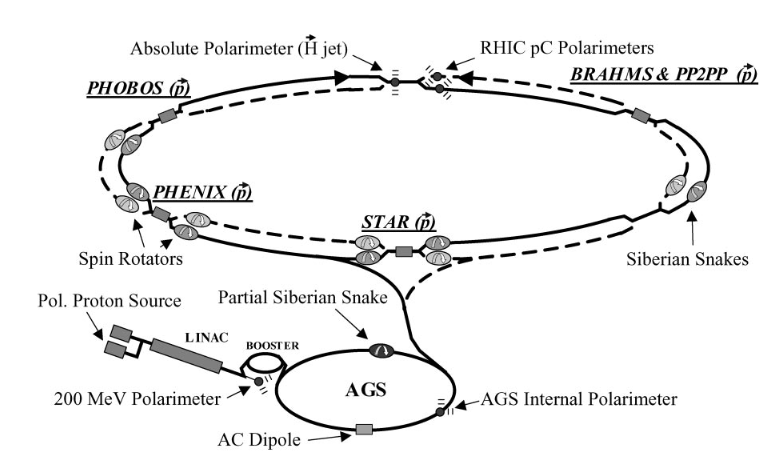
\includegraphics[scale=0.7]{Accelerating_System/protons_path}
		\caption{Η πορεία των πολωμένων πρωτονίων}
		\label{fig2.9}
	\end{figure}
	
	 Για παράδειγμα όταν η συχνότητα της μεταπτωτικής κίνσης του σπιν ισούται με την συχνότητα των μαγνητικών πεδίων που αλληλεπιδρούν με το σπιν, τότε προκαλείται ένας συντονισμός που μειώνει το ποσοστό των πολωμένων πρωτονίων της δέσμης.
 	Γενικότερα, οι κύριοι συντονισμοί που καταστρέφουν την πόλωση οφείλονται σε ατέλειες των μαγνητικών πεδίων και σε συντονισμούς οι οποίοι είναι εγγενείς στην αλληλεπίδραση σπιν-μαγνητικού πεδίου.
	Για παράδειγμα, αν υπάρχει μία ατέλεια του πεδίου η οποία διαταράσσει ελάχιστα το σπιν ενός διερχόμενου πρωτονίου περιστρέφοντάς προς τον άξονα της δέσμης, τότε κάθε φορά που ένας "παλμός" της δέσμης θα περνάει από εκείνο το σημείο της ατέλειας όλο και μεγαλύτερο ποσοστό των πολωμένων πρωτονίων θα χάσουν την πόλωσή τους. Αυτό το φαινόμενο καλείται \textit{συντονισμός αποπόλωσης} και εμφανίζεται σε ακέραιες τιμές του \textit{spin tune}, $v_{sp} = G\gamma =n, n\in\mathbb{N}$ 
 	%Ο δεύτερος συμβαίνει όταν $v_{sp} = G\gamma = 3k\pm v_y, k\in\mathbb{N}$ και $v_y$ είναι το εγκάρσιο \textit{betatron tune}.
 	
 
 
% 	Όταν η δέσμη περνάει μία περιοχή συντονισμού, τότε η τελική πόλωση $P_f$ σε σύγκριση με την αρχική $P_I$ δίνεται από την σχέση 
% 	\begin{align*}\label{eq2.8}
% 		\frac{P_f}{P_i} = 2 e^{-\frac{\pi r^2}{2\alpha}} - 1 \numberthis
% 	\end{align*}
%	
%	όπου α είναι η αλλαγή του \textit{spin tune} ανά ακτίνιο της τροχιάς και r είναι η ισχύς του συντονισμού. 
%	

%	Η αρχική πηγή πολωμένων πρωτονίων, παρέχει περίπου $10^12$ τέτοια σωματίδια σε κάθε παλμό ο οποίος εν συνεχεία επιταχύνεται στον AGS όπου μειώνονται τα πολωμένα πρωτόνια, καταλήγουν 2x$10^11$ στον RHIC.
%	Η πόλωση της δέσμης αλλάζει πρόσημο κάθε φορά που ικανοποιείται η συνθήκη συντονισμού $G\gamma = n, n\in\mathbb{N}$ και εν τέλει καταλήγουν στον RHIC 120 "παλμοί" από 2x$10^{11}$ πολωμένα πρωτόνια και με την \textit{emittance} της δέσμης λιγότερο από $20\mu m$.
		
	\begin{figure}[h!]
			\centering
			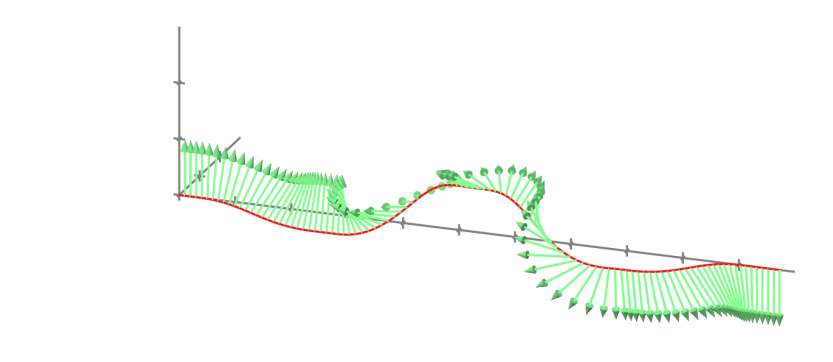
\includegraphics[scale=0.7]{Accelerating_System/traj_through_siberian}
			\caption{Η εξέλιξη της πόλωσης του spin κατά την διέλευση από έναν Siberian Snake μαγνήτη}
			\label{fig2.10}
		\end{figure}
		
	Στον RHIC, χρησιμοποιούνται οι μαγνήτες \textit{Siberian Snake} προκειμένου να διατηρήσουν την πόλωση της δέσμης.
	Αυτοί, προκαλούν συνολική περιστροφή της πόλωσης κατά 180$^o$ προς τον οάξονα της δέσμης, χωρίς να προκαλούν κάποια αλλοίωση στην τροχιά της δέσμης στο τέλος της διαδικασίας.
	Σε κάθε δαχτυλίδι του RHIC υπάρχουν 2 Siberian Snakes σε αντιδιαμετρικά σημεία, όπου ο καθένας αποτελείται από 4 υπεραγώγιμους ελικοειδής διπολικούς μαγνήτες μαγνητικού πεδίου εως 4Τ και μήκους 2.4m.

		
		
	Ακόμη, υπάρχουν 4 \textit{rotators}, οι οποίοι είναι μαγνήτες τοποθετημένοι σε κάθε δαχτυλίδι στις δύο άκρες του STAR (και άλλοι 4 για το PHENIX).
	Ο κάθε ένας τους αποτελείται από 4 διαδοχικά ελικοειδή δίπολα των οποίων τα πεδία ξεκινούν από κατακόρυφα και καταλήγουν διαμήκη. Έτσι κατά την είσοδο της δέσμης στην περιοχή αλληλεπίδρασης, υπάρχει η δυνατότητα να αλλάξουν την πόλωση από εγκάρσια σε διαμήκη ανάλογα με τις ανάγκες του πειράματος που δημιουργείται και κατά την έξοδό της να γίνει επαναφορά στην αρχική εγκάρσια πόλωση η οποία απαιτείται για την κίνηση εντός του RHIC.
	
	Οι διαφορετικές πολώσεις των πρωτονίων απαιτούνται για την μελέτη ασυμμετριών στις ενεργές διατομές. Για παράδειγμα, όπως θα δούμε στην συνέχεια, έχει βρεθεί διαφορά στις ενεργές διατομές συγκρούσεων προτονίων προς $\pi^0$ ανάλογα με το αν η πόλωση του σπιν των αρχικών πρωτονίων είναι κατακόρυφη προς τα πάνω ή προς τα κάτω.
	
	
		

\input{STAR_Detectors/Intro.tex}
\section{Forward Time Projection Chamber (FTPC)}

	Οι Time Projection Chambers (TPCs) είναι μία υποκατηγορία των θαλάμων ολίσθησης. 
	%Αποτελούνται από μία κοιλότητα η οποία περιέχει ένα αέριο και κάποια λεπτά σύρματα Εφαρμόζοντας ηλεκτρικό (μέσω διαφοράς δυναμικού στα σύρμαυα) και μαγνητικό πεδίο (από εξωτερικές πηγές) στον χώρο του αερίου μπορούμε να κατευθύνουμε τα φορτισμένα σωματίδια που υπάρχουν. 
	Αποτελούνται από μία κοιλότητα, στην περίπτωσή μας κυλινδρική, η οποία περιέχει ένα αεριο. Εντός αυτής της κοιλότητας επιβάλλουμε ηλεκτρικό πεδίο προς τις βάσεις του κυλίνδρου ( μέσω δύο μεγάλων ηλεκτροδίων ) και εξωτερικό μαγνητικό πεδίο παράλληλο με το ηλεκτρικό.
	Τότε, τα σωματίδια που περνάνε εντός της κοιλότητας και έχουν ιονιστική ικανότητα, υπό κατάλλες συνθήκες πίεσης και τιμές των πεδίων, ιονίζουν τα άτομα/μόρια του αερίου, δημιουργείται το φαινόμενο Townsted και ανιχνεύονται ως ένα σήμα μετά τους Multiwire  Proportion Chambers (MWPC)  στους Readout Chambers που είναι τοποθετημένοι σε μπλοκ στις δύο βάσεις. Οι MWPC είναι περιοχές που αποτελούνται από σύρματα-ανόδους πριν την τελική κάθοδο προκειμένου να ενισχυθεί το σήμα. Η λειτουργία τους θα περιγραφεί αναλυτικότερα στην συνέχεια όπου θα μελετήσουμε τους συμβατικούς TPC.
	Από την θέση που ανιχνεύονται τα σήματα μπορούμε να προσδιορίσουμε την προβολή της τροχιάς στις βάσεις και από την χρονική διαφορά που υπάρχει μεταξύ των ανιχνεύσεων μπορούμε να προσδιορίσουμε και την τρίτη συνιστώσα της τροχιάς. Ταυτόχρονα μπορούμε να ταυτοποιήσουμε τα σωματίδια μέσω της ενέργειας που εναποθέτουν στο αεριο μέσω ιονισμού ( Καμπύλη Bethe-Bloch).
	
	
	 Συγκεκριμένα οι FTPC του STAR έχουν κάποιες ιδιαιτερότητες οι οποίες προέκυψαν προκειμένου να επεκταθεί η κάλυψη σε μεγαλύτερες τιμές pseudorapidity $2.5<|\eta|<4.0$ καθώς υπήρχε η ανάγκη για κάλυψή τους αφού παράγονταν υψηλές πυκνότητες σωματιδίων με μεγάλη η. Η pseudorapidity πρόκειται για μία χωρική συντεταγμένη η οποία περιγράφει την γωνία ενός σωματιδίου που παράγεται από τις κρούσεις ως προς την αρχική δέσμη και ορίζεται ως 
	 	\begin{equation}\label{eq3.1}
	 		\eta = -ln\left(tan(\theta/2)\right) = arctanh(\frac{p_L}{|\bm{p}|} )
	 	\end{equation}
	 	
	 	όπου θ η γωνία δέσμης-ορμής σωματιδίου, $|\bm{p}|$ το μέτρο της ορμής του και $p_L$ η συνιστώσα της ορμής που είναι παράλληλη στην δέσμη. Άρα οι FTPC στόχευαν  να βελτιώσουν τον χαρακτηρισμό των γεγονότων στο STAR ανιχνεύοντας σωματίδια με μιρκή γωνία θ προς την δέσμη και επιτρέποντας την μελέτη μη συμμετρικών συκγρούσεων όπως Au-p. 
	 	
	 	\subsection{Η λειτουργία των FTPC}

	Οι FTCP του STAR διαφέρουν σε μερικά σημεία από έναν απλό TPC. Η ιδέα γι' αυτούς καθορίστηκε από δύο παράγοντες. Πρώτον, την ανάγκη για κάλυψη μεγάλων η και δεύτερον τον περιορισμένο χώρο μεταξύ δέσμης και του κανονικού TPC που υπάρχει μετά τον FTPC. 
	Όπως φαίνεται στην Εικόνα (\ref{fig3.2}) πρόκειται για ένα κυλινδρικό θάλαμο εσωτερικής ακτίνας $R_{FTCP,in}=7.73cm$, εξωτερικής ακτίνες $R_{FTCP,out}=30.05cm$, μήκους $L_{FTCP}=120cm$ με ακτινικό πεδίο ολίσθησης που προκαλείται από την διαφορά δυναμικού $10-15kV$ μεταξύ του εσωτερικού και εξωτερικού ηλεκτροδίου. Έτσι, οι  Readout Chambers είναι τοποθετημένοι σε 5 κυλινδρικά δαχτυλίδια στην εξωτερική επιφάνεια τoυ FTCP. Καθένα από τα δαχτυλίδια έχει 6 Readout Chambers.
	
	\begin{figure}[h!]
		\centering
		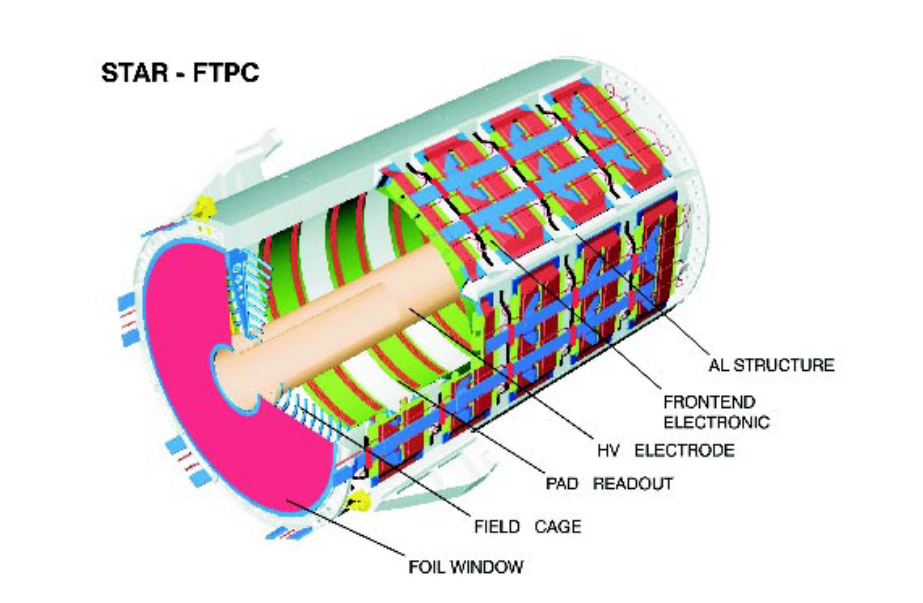
\includegraphics[scale=0.5]{STAR_Detectors/STAR_FTCP.png}
		\caption{Η δομή του FTCP}
		\label{fig3.2}
	\end{figure}		 	
	 	
	 	
	 Μία από τις ιδιαιτερότητες του FTPC είναι ότι η ολίσθηση των ηλεκτρονίων γίνεται ακτινικά, δηλαδή κάθετα στο μαγνητικό πεδίο, προκειμένου να να βελτιωθεί η διακριση μεταξύ δύο τροχιών κοντά στην δέσμη όπου η πυκνότητα των σωματιδίων είναι μεγαλύτερη. Η προβολή της τροχιάς στην βάση του θα μείωνε την διακριτική του ικανότητα καθώς ο FTPC βρίσκεται πολύ κοντά στην δέσμη και τα σωματίδια δεν θα προλάβαιναν να διαχωριστούν επαρκώς. Την εποχή που κατασκευάστηκε ήταν ο μοναδικός TCP που μπορούσε να διακρίνει δύο τροχιές με ακρίβεια 1-2mm. Ακόμη, έχουν χρησιμοποιηθεί καμπύλοι Readout Chambers (Εικόνα (\ref{fig3.4}) για να διατηρηθεί το ακτινικό ηλεκτρικό πεδίο όσο πιο αναλοίωτο γίνεται. 
	 
	 
	 Το μείγμα αερίων που χρησιμοποιείται είναι Ar/$CO_2$ (50\%-50\%). Αυτό έχει τα πλεονεκτήματα ότι δεν αλλοιώνεται με τον χρόνο, είναι χημικά αδρανές, δεν είναι εύκλεκτο και έχει μικρό συντελεστή διάχυσης για τα ηλεκτρόνια. Το τελευταίο βελτιώνει την χωρική διακριτική ικανότητα, δεδομένου ότι αυτή δίνεται από την σχέση 
	 	\begin{equation}\label{eq3.2}
	 		\sigma_x = \frac{\sigma_D\sqrt{L}}{\sqrt{n}}
	 	\end{equation}
	 όπου $\sigma_D$ ο συντελεστή διάχυσης για τα ηλεκτρόνια, $L$ το μήκος που ταξιδεύουν εντός του αερίου.
	 
	 \begin{figure}[h!]
	 	\centering 
	 	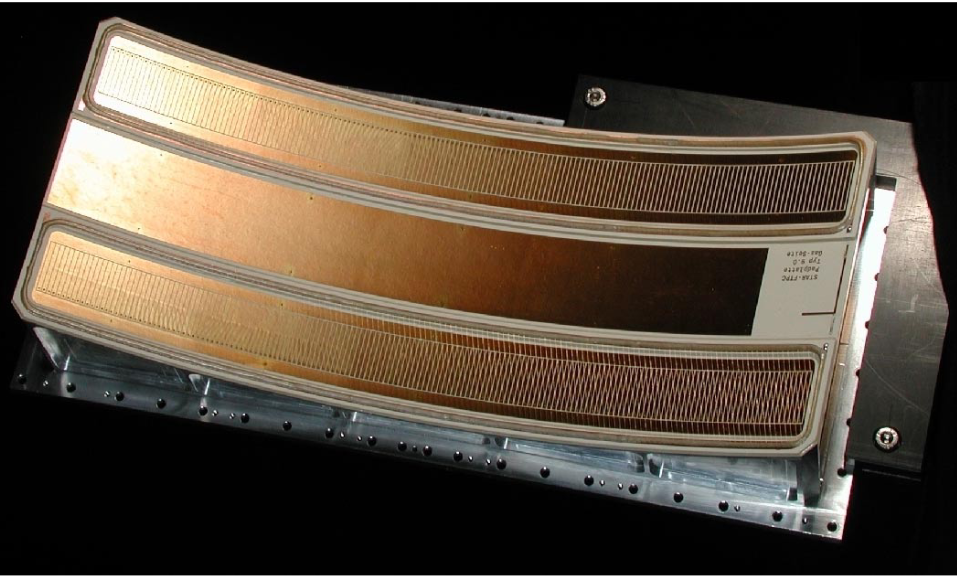
\includegraphics[scale=0.5]{STAR_Detectors/FTPC_readout_chamber}
	 	\caption{Readout Chamber του FTPC. Η ακτίνα καμπυλότητάς του είναι 305mm και έχει δύο συστοιχίες από 160 pad η κάθε μία. }
	 	\label{fig3.3}
	 \end{figure}
	 
	 Προκειμένου να υπάρχει παραγωγή ενός χρήσιμου σήματος από τις καθόδους,  ακριβώς πίσω τους υπάρχουν ηλεκτρονικά, που αποτελούνται συνολικά από 19.200 κανάλια, και τα οποίο λέγονται Front End Electronics (FEΕ). Αυτά ενισχύουν, διαμορφώνουν και ψηφιοποιούν το σήμα. Κάθε pad είναι συνδεδεμένο με έναν προενισχυτή ο οποίος μετά από κάποια στάδια στέλει το σήμα στο Data Aquisition System (DAQ).
	 
	 Κατά την λειτουργία, είναι εμφανές πως οι συνθήκες που επικρατούν δεν είναι συνεχώς ιδανικές και όπως είχαν αρχικά σχεδιαστεί. Γι' αυτό υπάρχει ένα σύστημα Nd:YAG Laser που βοηθά στην βαθμονόμηση και εξετάζει την λειτουργικότητα των FTPC ανεξάρτητα του RHIC. Συγκεκριμένα, προκαλεί ευθύγραμμους ιονισμούς από γνωστές θέσεις προκειμένου να εντοπιστούν τυχών χωρικές διαταραχές που οφείλονται στα μηχανικά χαρακτηριστικά του FTPC ή σε ατέλειες του πεδίου. Βοηθά επίσης στην βαθμονόμηση των ταχυτήτων ολίσθησης του αερίου.
	 	
	 Αφού πλέον μπορούμε να ανιχνεύσουμε τις τροχιές των σωματιδίων μέσω των σημάτων στις ανόδους και να βαθμονομήσουμε το σύστημά μας με την βοήθεια των Laser, θα πρέπει να μπορούμε να επανακατασκευάσουμε τις τροχιές.
	  Το πρώτο στάδιο είναι να εντοπίσουμε τα σημεία των ανόδων που έδωσαν σήμα στα ηλεκτρονικά. Αυτό γίνεται μέσω ενός προγράμματος που διαβάζοντας τα δεδομένα που δίνονται από τα pads, τον χρόνο ολίσθησης και τις απαραίτητες διορθώσεις λόγω της ύπαρξης μαγνητικού πεδίου το οποίο αλλοιώνει την χωρική διακριτική ικανότητα, αντιστοιχεί τις περιοχές μη μηδενικού φορτίου σε συντεταγμένες θέσης. 
	  Το δευτερο βήμα είναι να ομαδοποιήσουμε αυτές τις θέσεις μη μηδενικού φορτίου. Κατασκευάζοντας τις τροχιές, βρίσκει το σημείο τομής τους, το οποίο θεωρούμε ότι είναι το σημείο από το οποίο προήλθαν τα σωματίδια και έπειτα συνδυάζοντας αυτό το σημείο με το μαγνητικό πεδίο υπολογίζονται οι ορμές των σωματιδίων. Μία τέτοια ανακατασκευή φαίνεται στην Εικόνα (\ref{fig3.4}), όπου από 14.745 χωρικά σημεία έχουν ανακασκευασθεί περίπου 1000 τροχιές σωματιδίων σε λιγότερο από 2 δευτερόλεπτα.
	  
	  \begin{figure}[h!]
	  		\centering
	  		\includegraphics[scale=0.5]{STAR_Detectors/FTPC_Reconstruction}	
	  		\caption{Ανακατασκευασμένες τροχιές από τον FTCP προερχόμενες από γεγονότα Au-Au $\sqrt{S}=200GeV$}  
	  		\label{fig3.4}
	  \end{figure}
	  
	  %Συνολικά, η χωρική διακριτική ικανότητα των FTCP είναι 100$\mu m$, η διακριτική ικανότητα στην ορμή βρίσκεται από προσομοίωση 12-15\% 
\section{Time Projection Chamber (TPC)}

	Στο αμέσως επόμενο στρώμα απο τον FTPC υπάρχει ένας τυπικός TPC (αυτός είναι και ο βασικός ανιχνευτής του STAR), που ανακατασκευάζει την τρισδιάστατη τροχιά των φορτισμένων σωματιδίων που παράγονται από τα γεγονότα κρούσεων στον RHIC. 
	Σε μία κεντρική κρούση Au-Au παράγονται περίπου 1000 πρωτογενή σωματίδια τα οποία με την σειρά τους αλληλεπιδρούν με το αέριο στο εσωτερικό του TPC και γεννούν  δευτερογενή σωματίδια. 
	Ο TPC μπορεί να ταυτοποιήσει τα δευτερογενή, αλλά και να ανακατσκευάσει περίπου 3000 από τις τροχιές τους, που ενδεχομένως θα οδηγήσουν σε συμπεράσματα για την αρχική κρούση. Μπορεί να ανακασκευάσει τροχιές από σωματίδια με μέση ορμή $100MeV/c<\braket{p}<1GeV/c$ και να μετρήσει την ορμή σωματιδίων με $100MeV/c<\braket{p}<30GeV/c$.
	
	Γεωμετρικά, πρόκειται για έναν κυλινδρικό θάλαμο με μήκος 4.2m και ακτίνας 4m ο οποίος περιέχει ένα μίγμα αερίων και είναι τοποθετημένος στο εσωτερικό ενός σωληνοειδούς με μαγνητικό πεδίο εως 0.5Τ. Επίσης, το εσωτερικό του χωρίζεται στα δύο από μία λεπτή μεμβράνη σε υψηλή τάση μεταξύ της οποίας και των άκρων επιβάλλουμε ηλεκτρικό πεδίο της τάξης των $~135V/cm$.
	
\begin{figure}[h!]
    \centering
    \subfloat[\centering Γεωμετρία]{{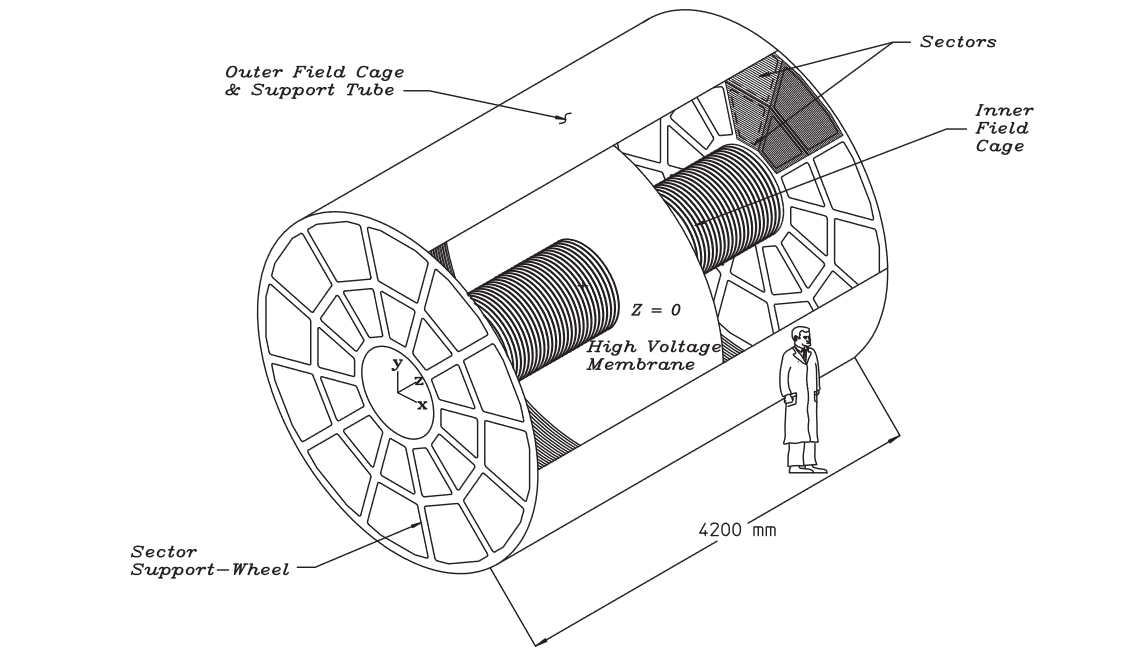
\includegraphics[scale=0.35]{STAR_Detectors/STAR_TPC} }}%
    \qquad
    \subfloat[\centering Φωτογραφία από το εσωτερικό]{{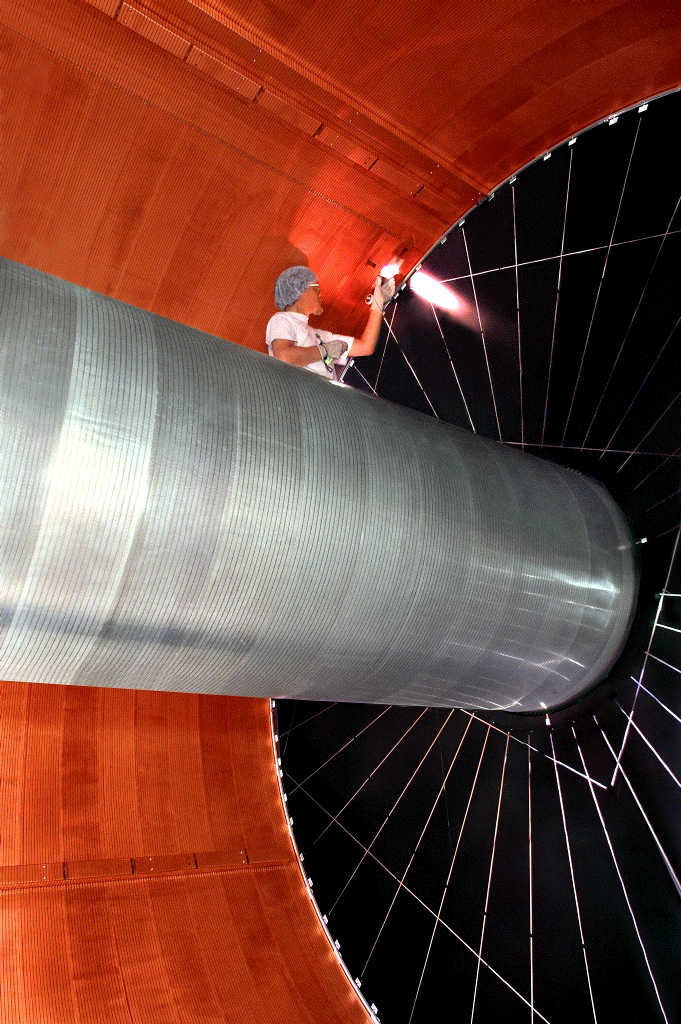
\includegraphics[width=4.5cm]{STAR_Detectors/InsideTpc} }}%
    \caption{O TPC }%
    \label{fig3.6}%
\end{figure}					
	 
	 Η τροχιά των σωματιδίων που ανιχνεύονται και χρησιμοποιούνται στην ανακατασκευή εξαρτάται από το ηλεκτρικό πεδίο. Άρα, δεδομένου ότι αυτά ταξιδεύουν έως και 2.1m, μία μικρή εκτροπή τους, που να οφείλεται σε ανομοιογένεια του πεδίου, μπορεί να οδηγήσει σε μεγάλη αλλοίωση της τροχιάς και κατ' επέκταση σε κακή ανακασκευή.
	Επομένως, η ομογένεια του ηλεκτρικού πεδίου είναι κρίσιμη καθώς η ανακατασκευή των τροχιών πρέπει γίνεται με ακρίβεια καλύτερη του χιλιοστού.
	
	Εξαιτίας του ηλεκτρικού πεδίου, τα δευτερογενή ηλεκτρόνια που παράγονται ολισθαίνουν προς τις βάσεις του κυλίνδρου όπου και ανιχνεύονται από το Σύστημα Ανάγνωσης (Readout System). 
	Αυτό βασίζεται σε Multiwire Proportional Chambers (MWPC) με Readout Pads. Oι MWPC έχουν συρμάτινες ανόδους ακτίνας 20μm που παρέχουν ενίσχυση σήματος. Το επαγόμενο φορτίο από μία χιονοστιβάδα μοιράζεται σε πολλά γειτονικά \textcolor{red}{pads} για ακριβέστερη ανακατασκευή.  Συνολικά υπάρχουν 136.608 pads.
	
	Το αέριο εντός του TPC είναι συνήθως μίγμα 10\%μεθανίου - 90\% Αργού σε πίεση 2mbar μεγαλύτερη της ατμοσφαιρικής. Ένα βασικό του χαρακτηριστικό είναι το ότι έχει τυπική ταχύτητα ολίσθησης που μεγιστοποιείται σε μικρές τιμές ηλεκτρικού πεδίου.
	
	Η διακριτική ικανότητα της θέσης καθορίζεται από την διάχυση των δευτερογενών ηλεκτρονίων ενώ η δυνατότητα ανίχνευσης σωματιδίων, που βασίζεται στην απώλεια ενέργειας, περιορίζεται από τις διακυμάνσεις στον ιονισμό και το πεπερασμένο μέγεθος του θαλάμου καθώς πολλά από αυτά δεν θα προλάβουν να εναποθέσουν όλη τους την ενέργεια.
	
\subsection{Μίγμα Αερίων}
	Ας ξεκινήσουμε από τα πιό απλά, ή τουλάχιστον αυτά που θα παρουσιαστούν ως πιό απλά σε αυτή την εργασία. Τα μίγματα αερίων που χρησιμοποιούνται είναι το 10\%μεθανίου - 90\% Αργού και το 50\%He+50\% $C_2H_6$. Τα εν λόγω αέρια επιλέχθηκαν με κριτήρια όπως η καθαρότητα που μπορεί να επιτευγχθεί, η εύκολη διατήρησή της, η ταχύτητα ολίσθησης, το κόστος, η ασφάλεια.
	
	Τα αέρια, συνολικού όγκου 50.000lt, κυκλοφορούν σε ένα κλειστό σύστημα με ροή 36.000lt/hr, όπου διαρκώς φιλτράρονται και απομακρύνται τα ξένα στοιχεια. Για παράδειγμα, αν έχουμε στοιχεία υψηλής ηλεκτραρνητικότητας τότε αυτά θα επιβραδύνουν τα δευτερογενή ηλεκτρόνια που θέλουμε να ανιχνεύσουμε, αλλοιώνοντας τα σήματά μας. Έτσι, είναι αναγκαίο το να κρατάμε τα επίπεδα οξυγόνου και νερού κάτω από 100ppm και 10ppm  αντίστοιχα. 	
	
	Χαρακτηριστικά του αερίου χρησιμοποιούνται επίσης για τον σχεδιασμό άλλων σημείων του TPC. Ενδεικτικά, αν ένα σωματίδιο ταξιδέψει όλο το δυνατό μήκος των 2.10m τότε η κάθετη διάχυση είναι $\sigma_T=3.3mm$ και αυτό μας καθορίζει την κλίμακα του συστήματος ανάγνωσης στα άκρα του TPC.
	% ενώ η διαμήκης $\sigma_L=5.2mm$ η οποία για ταχύτητα ολίσθησης 5.45cm/μs αντιστοιχεί σε χρόνο 230ns. 

	
	Η ταχύτητα ολίσθησης στο αέριο μεθανίου -  Αργού συναρτήσει του λόγου του πεδίου προς την πίεση για διάφορες τιμές συγκεντρώσεων φαίνεται στην Εικόνα (\ref{fig3.7}). Είναι λογικό να επιλέξουμε πεδίο τέτοιο, ώστε να είναι κοντά στο μέγιστο των καμπυλών. Αυτό, προκειμένου να εξασφαλίσυομε ότι η ταχύτηα θα είναι όσο λιγότερο ευαίσθητη σε μικροαλλαγές πίεσης και πεδίου. Παρ' όλα αυτά, επειδή στον TPC του STAR υπάρχει ένα σύστημα αυτόματου ελέγχου της ταχύτηας ολίσθησης που μετρά την αντίστοιχη ταχύτητα σωματιδίων που προέρχονται από ιονισμό μέσω Laser, γίνονται αυτόματες μικροδιορθώσεις στο ηλεκτρικό πεδίο για να εξισορροπηθούν οι μεταβολές της λόγω πίεσης. Επομένως, δεν θα πρέπει να υπάρχει η μέγιστη ταχύτητα, αλλά λίγο μικρότερη. Αυτό είναι αναγκαίο για την λειτουργία του συστήματος αυτόματου ελέγχου καθώς αν λειτουργούσαμε με την μέγιστη και εκείνο μετρούσε μία μείωσή της δεν θα ήταν ικανό να καθορίσει προς τα ποιά μεριά της καμπύλης συνέβη η μείωση, άρα δεν θα μπορούσε να καθορίσει κατάλληλα την αλλαγή στο πεδίο.
	
	%\begin{figure}[h!]
	%	\centering 
	%	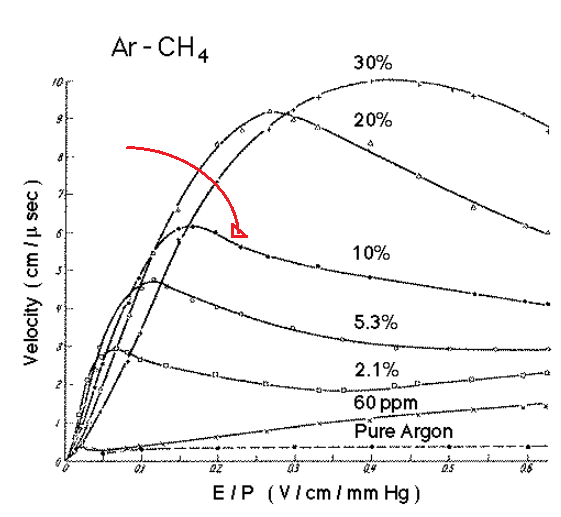
\includegraphics[scale=0.45]{STAR_Detectors/Gases}
	%\caption{Συνάρτηση της ταχύτητας ολίσθησης ως προς τον λόγο πεδίου/Πίεση }
	%	\label{fig3.7}
	%\end{figure}
	\begin{figure}[h!]
		\centering
		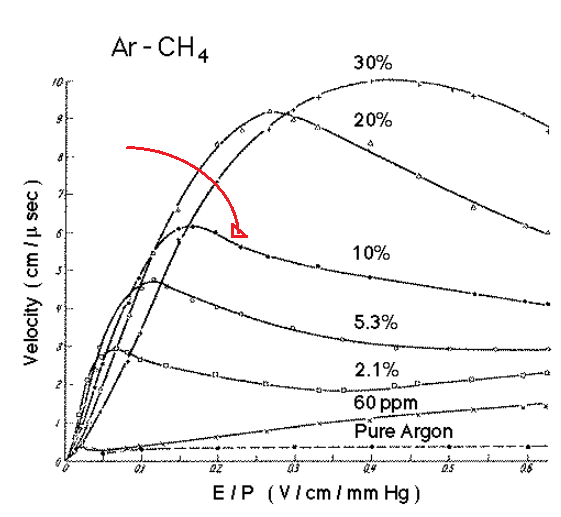
\includegraphics[scale=0.45]{STAR_Detectors/Gases}
   	\caption{Συνάρτηση της ταχύτητας ολίσθησης ως προς τον λόγο πεδίου/Πίεση }
		\label{fig3.7}
	\end{figure}	
	
\subsection{ Field Cage (Κυλινδρικό Κέλυφος)  }
	Tώρα θα ασχοληθούμε με τα γεωμετρικά όρια του TPC, τα οποία καθορίζουν τα χαρακτηριστικά του. Θα ξεκινήσουμε από αυτά που δεν περιλαμβάνουν τις συσκευές ανίχνευσης, δηλαδή με το κυλινδρικό κέλυφος και την εσωτερική άνοδο και στην συνέχεια θα ασχοληθούμε με τις βάσεις. Το σύστημα όλων των τοιχωμάτων επιβάλλει τις συνοριακές συνθήκες για το ομογενές ηλεκτρικό πεδίο, επομένως είναι σημαντικό να τοποθετηθούν με ακρίβεια. Για παράδειγμα η κεντρική μεμβράνη θα πρέπει να είναι ακριβώς παράλληλη με τις βάσεις.
	
	Αρχικά, σχετικά με την κεντρική μεμβράνη (Cenral Membrane - CM ). Αυτη πρόκειται για έναν κυκλικό φλοιό 70$\mu m$ από άνθρακα με επίστρωση από το πολυμερές Kapton, έχει μία εσωτερική οπή για να εφαρμόζει στον εσωτερικό κύλινδρο, και  της  εφαρμόζουμε δυναμικό 28kV σε αντίθεση με τις βάσεις που είναι γειωμένες. Άρα η CM είναι η ανοδος. Όμως, όπως έχει αναφερθεί, θέλουμε τον ακριβή προσδιορισμό του πεδίου στο εσωτερικό του TPC, υπάρχουν τοποθετημένες σε κάθε πλευράς της μεμβράνης 36 λωρίδες αλουμινίου. Το αλουμίνιο είναι ένα υλικό με χαμηλό έργο εξόδου. Έτσι, αν το στοχεύσουμε με UV-Laser θα προκαλέσουμε την εξαγωγή ηλεκτρονίων από αυτό. Μετρώντας αυτά τα ηλεκτρόνια μπορεί να γίνει η βαθμονόμηση του συστήματος προσδιορίζοντας ακριβώς τις θέσεις των λωρίδων αλουμινίου άρα των ορίων του θαλάμου και κατ' επέκταση τις μεταβολές στο πεδίο.
	
	Ο εσωτερικός και ο εξωτερικός κύλινδρος εξυπηρετούν δύο σκοπούς,  περιορίζουν το αερίο και θέτουν τις Συνοριακές Συνθήκες για το πεδίο. Η μηχανική τους σχεδίαση έγινε με στόχο την ελάττωση της μάζας και την μείωση των σκεδάσεων Coulomb στο εσωτερικό τους που αλλοιώνουν τις τροχιές. 
	Τα τοιχώματά τους δεν πρόκειται για απλά μεταλλικά υλικά αλλά για διαδοχικά στρώματα όπως φαίνεται στην Εικόνα (\ref{fig3.8}). 
	Πηγαίνοντας από έξω προς τα μέσα, η δομή έιναι Μεταλλικό στρώμα-Πολυμερές Kampton-Μεταλλικό στρώμα	
	Στο ενδιάμεσο αυτών υπάρχει το υλικό NOMEX σε σχήμα κυρηθρών το οποίο είναι ένα διηλεκτρικό, ελφρύ υλικό με μεγάλη αντοχή. 
	Κάθε 1.5mm υπάρχουν χαραγές προκειμένου να δημιουργηθούν ηλεκτρικά απομονωμένες περιοχές.
	% και να παρέχεται με ασφάλεια η τάση στα διαφορετικά δαχτυλίδια.
	 Η ελαχιστοποίηση της απόστασης των χαραγών στο 1.5mm είναι σημαντική τόσο για την μηχανική αντοχή, όσο και για την εκθεση του Kapton στο αέριο  η οποία μπορεί να αλλοιώσει το πεδίο εξαιτίας της τοπικής συγκέντρωσης φορτίων.
	
	
	\begin{figure}[h!]
			\centering 
			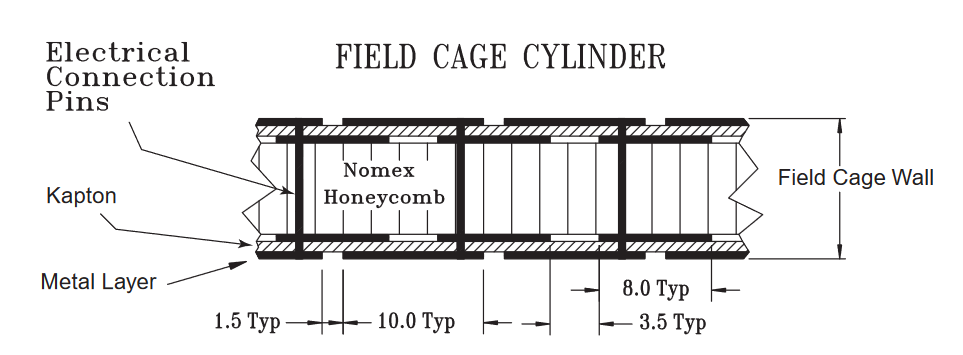
\includegraphics[scale=0.4]{STAR_Detectors/Inner_field_cage_wall}
			\caption{Το τοίχωμα του εσωτερικού φλοιού με διαστάσεις σε mm}
			\label{fig3.8}
		\end{figure}
		
	Ένα ακόμη σημαντικό σημείο είναι η ελαχιστοποίηση του υλικού στον εσωτερικό φλοιό καθώς εκεί λόγω της υψηλής πυκνότητας σωματιδίων είναι κρίσιμο να μειωθουν κατά το δυνατό οι αλληλεπιδράσεις Coulomb στο εσωτερικό του υλικού για την ακριβέστερη ανακατασκευή των τροχιών. 
	Στον εσωτερικό κύλινδρο, τα μεταλλικά κομμάτια είναι κατασκευασμένα από αλουμίνιο 12.8mm. με 0.5\% του radiation length $X_0$, ενώ στον εξωτερικό φλοιό, χάριν απλότητας, χρησιμοποιήθηκαν 10mm χαλκού σε 1.3\%$X_0$.
	
	Για την ηλεκτρική μόνωση των δύο φλοιών από τα γειτονικά τους κομμάτια χρησιμοποιούνται αέρια. Τα πλεονεκτήματα των αερίων έναντι των στερεών, είναι πως μειώνουν την δημιουργία δευτερογενών σωματιδίων σε αυτή την περιοχή όπου δεν μπορούν να ανιχνευτούν, ενώ ταυτόχρονα δεν υπάρχει η πιθανότητα για μόνιμη ζημία ή καταστροφή τους. Δηλαδή, μπορούν ανά πάσα στιγμή να ανανεωθούν χωρίς ιδιαίτερα υψηλό κόστος.
	
\subsection{End Caps (Βάσεις του Κελύφους)}

 Οι βάσεις είναι γειωμένες, με αποτέλεσμα το πεδίο στο δεξί και στο αριστερό μέρος του TPC  να είναι αντίθετο. 
 Σε αυτές είναι τοποθετημένοι οι  Mulitwire Proportional Chambers (MWPC) που πρόκειται για τους Readout Chambers που αποτελούν το πρώτο βήμα στην διαδικασία παραγωγής αξιοποιήσιμων σημάτων. Οι MWPC είναι αρθρωτοί θάλαμοι, δηλαδή διαφορετικές μονάδες που ενώνονται σε αλουμινένιες βάσεις. Η κυκλική βάση είναι χωρισμένη σε 12 τομείς που απέχουν 3mm μεταξύ τους και σε αυτούς είναι τοποθετημένοι οι εν λόγω θάλαμοι.  
	
	Ο κάθε MWPC αποτελείται από ένα επίπεδο pad και τρία επίπεδα από λεπτά σύρματα παράλληλα με το τοίχωμα (Εικόνα (\ref{fig3.9}). Το επίπεδο pad βρίσκεται στην εξωτερική πλευρά. Αμέσως δίπλα του υπάρχει το επίπεδο συρμάτων ανόδου, μετά τα \textcolor{red}{γειωμένα} σύρματα (σύρματα θωράκισης) και τέλος τα  σύρματα gating. Η κατεύθυνση των συρμάτων έχει επιλεγχθεί έτσι ώστε να βελτιστοποιείται η μέτρηση της ορμής των σωματιδίων με μέγιστη κάθετη ορμή $p_T$ των οποίων οι τροχιές είναι σχεδόν ευθείες που πηγάζουν από το σημείο κρούσης.
	%Είναι λοιπόν τοποθετημένα κάθετα στις τροχιές των σωματιδίων διότι τα σύρματα έχουν καλύτερη διακριτική ικανότητα κατά μήκος τους και όχι κατά την κατεύθυνση που διαχωρίζεται το ένα από το άλλο.
	Ομοίως, οι διαστάσεις των επίπεδων pad είναι τέτοιες, ώστε να βελτιστοποιείται η χωρική διακριτική ικανότητα των τροχιών. Πιό συγκεκριμένα, το κάθε pad έχει διαστάσεις ώστε το μεγαλύτερο μέρος φορτίου που δημιουργείται γύρω από μία άνοδο κατά μία χιονοστιβάδα Townsend να ανιχνεύεται μόνο από 3 pads. 
	
\begin{figure}[h!]
		\centering 
		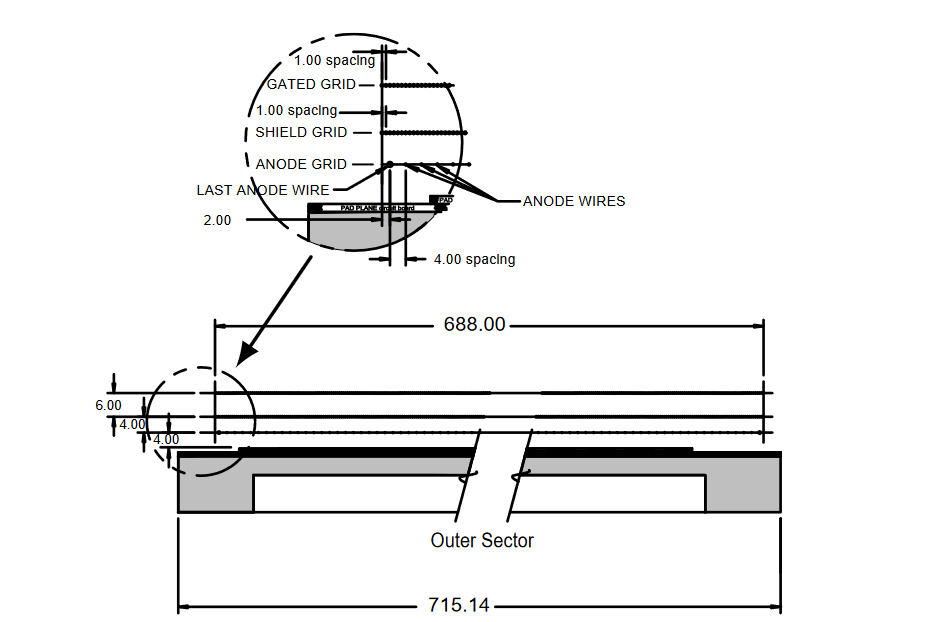
\includegraphics[scale=0.3]{STAR_Detectors/Readout_Sector}
		\caption{ Ένας MWPC του STAR του εξωτερικού τομέα. Οι διαστάσεις είναι σε mm.}
		\label{fig3.9}
	\end{figure}
		
	
	Υπάρχουν δύο υπό-τομείς με διαφορετική διαρρύθμιση των pads. Στον εξωτερικό, τα pads είναι πιό πυκνά για να δώσουν καλύτερη διακριτική ικανότητα στην απώλεια $dE/dx$, καθώς η μεγάλη πυκνότητα των pads εξασφαλίζει ανίχνευση και διάκριση μεγαλύτερου αριθμού σωματιδίων. H διαρρύθμιση εδώ είναι σε ένα τετραγωνικό πυκνό  πλέγμα. 
	Τα εσωτερικά pads είναι τοποθετημένα με διαφορετικό τρόπο. Εκεί, δεν μας ενδιαφέρει τόσο ο ακριβής προσδιορισμός της τροχιάς και της $dE/dX$, όσο το να διακρίνουμε δύο τροχιές. Η ελλάτωση των προσδοκιών εγκειται στο γεγονός ότι όντας κοντύτερα στα σημεία σύγκρουσης, η πυκνότητα των τροχιών είναι πολύ μεγαλύτερη άρα αυξάνεται η δυσκολία ανακατασκευής τους. Γι' αυτούς τους λόγους είναι τοποθετημένα σε διακριτές γραμμές .
	
	Μένει τώρα να ασχοληθούμε με τον σκοπό που εξυπηρετούν τα επίπεδα συρμάτων. 
Αρχικά, στην περιοχή γύρω από τα ανοδικά καλώδια, το ηλεκτρικό πεδίο επιταχύνει τα ηλεκτρόνια, αυξάνοντας το πλήθος τους μέσω Townsend, αφού υπάρχει επιπλέον ηλεκτρικό πεδίο μεταξύ αυτών και των pads που λειτουργούν ως κάθοδοι.
% αλλάζει κατεύθυνση και παύει να είναι παράλληλο με το μαγνητικό. Τότε ενισχύεται η ολίσθηση $\bm{E}\times\bm{B}$ και τα ηλεκτρόνια κινούνται προς τις ανόδους.
	Το πλέγμα θωράκισης έχει στόχο να περιορίζει το ηλεκτρικό πεδίο ανόδων-καθόδων εντός την περιοχής ενίσχυσης των ηλεκτρονίων. 
	Τέλος, το εξωτερικό πλέγμα, Gating Grid, λειτουργεί ως σύστημα ελέγχου των ηλεκτρονίων που εισέρχονται από τον θάλαμο ολίσθησης στον MWCP. Η τυπική του κατάσταση είναι να είναι "κλειστό" και να μην επιτρέπει την διέλευση των ηλεκτρονίων που έχουν παραχθεί από φορτισμένα σωματίδια στον θάλαμο ολίσθης.  Όταν όμως υπάρχει κάποιο ενδιαφέρον γεγονός, τότε "ανοίγει" και επιτρέπει την διέλευσή τους.
	
	Επίσης, στην περιοχή ενίσχυσης παράγεται μεγάλο πλήθος ιόντων που δημιουργούν μία χωρική κατανομή φορτίου η οποία αν περάσει στον κύριο θάλαμο ολίσθησης θα προκαλέσει ανεπιθύμητες διαταραχές στο ηλεκτρικό του πεδίο.  Έτσι,
ο δεύτερος σκοπός του gating grid είναι να εμποδίζει την διαφυγή των ιόντων. Όταν είναι σε "ανοιχτή" καταάσταση, τότε τα ιόντα λόγω μεγάλης μάζας, άρα μικρής ταχύτητας ολίσθης, δεν προφταίνουν να διαφύγουν, ενώ όταν είναι σε "κλειστή" κατάσταση παγιδεύονται από αυτό.
\vspace{-0.1cm}
\subsection{Η Επίδοση του TPC}
\subsubsection{Ανακατασκευή των x-y-z Θέσεων}
	H τροχιά ενός πρωτογενούς σωματιδίου ανακατασκευάζεται μέσω των συγκροτημάτων (clusters) δευτερογενών ηλεκτρονίων που ανιχνεύονται. Ο άξονας x ορίζεται ως ο άξονας που είναι παράλληλος στις σειρές των pads ενώ ο y επεκτέινεται από την δέσμη εως την μέση των σειρών με τα pads.
	Άρα για τον προσδιορισμό της x θέσης ψάχνουμε για ιονισμό κοντά σε γειτονικά pads της ίδια σειράς. Όταν δύο τροχιές συμπίπτουν μεταξύ τους, τότε τα pads θα ανιχνεύσουν ιονισμό που προέρχεται και από τις δύο. Ο διαχωρισμός τους γίνεται με κατάλληλους αλογρίθμους ενώ είναι αδύνατος ο προσδιορισμός της dE/dx. Περίπου το 30\% των τροχιών επικαλύπτωνται σε συγκρούσεις Au-Au 200GeV.
	Ο άξονας z ορίζεται ως ο άξονας που συμπίπτει με την δέσμη. Η z συντεταγμένη καθορίζεται από την μέτρηση του χρόνου ολίσθησης των cluster δευτερογενών ηλεκτρονίων. 
	%Ο χρόνος άφιξης των cluster υπολογίζεται μετρώντας τον χρόνο αφιξης των ηλεκτρονίνων σε ομάδες και παίρνωντας μέσο όρο.
	Έπειτα από την εύρεση των θέσεων του cluster των δευτερογενών ηλεκτρονίων, ένας αλγόριθμος ανακατασκευάζει όλη την τροχιά του σωματιδίου και έπειτα από αυτήν μπορούμε να εξάγουμε πληροφορίες για την ορμή του.

	Προφανώς, υπάρχουν διάφοροι παράγοντες που επιδεινώνουν την αρκίβεια προσδιορισμού της τροχιάς και οι οποίοι πρέπει να ληφθούν υπ' όψιν σε μετέπειτα διορθώσεις. Ενδεικτικά, μερικοί από αυτούς είναι η ανομοιογένεια το μαγνητικού πεδίου, η διαφορά στην γεωμετρία του εσωτερικού από του εξωτερικού τομέα με MWPC, η απόκλιση της καθόδου από την επιπεδότητα, η γωνιακή απόκλιση των \textbf{B, E} πεδίων και η συγκέντωση χωρικού φορτίου στον TPC. Οι παράγοντες αυτοί οδηγούν όλοι σε μία διόρθωση της θέσης της τάξης του 0.01cm.

\subsubsection{Ταυτοποίηση Σωματιδίων Μέσω της dE/dx}
	
	Η μέθοδος ταυτοποίησης των σωματιδίων μέσω της καμπύλης Bethe-Bloch λειτουργεί πιό αποδοτικά για σωματίδια με μικρή $p_T$ ορμή.  Όπως φαίνεται και στην Εικόνα (\ref{fig3.}), όσο μεγαλώνει η ορμή, τόσο μειώνεται η εξάρτηση της dE/dx από την μάζα του σωματιδίου. Άρα, η εναπόθεση ενέργειας είναι παρόμοια για όλα τα σωματίδια καθιστώντας αδύνατη την ανίχνευσή τους.
	
		Ο στόχος του STAR είναι η δυνατότητα για διάκριση μεταξύ Καονίων και πρωτονίων έως 1.2GeV/c κάτι που απαιτεί $\sigma_{dE/dx}$ διακριτική ικανότητα 7\%. Αυτή εξαρτάται από την ενίσχυση των φαινομένων Townsend άρα από την πίεση. Υπάρχει ένα σύστημα ελέγχου της πίεσης που μεριμνά για την διατήρηση της ενίσχυσης στα επιθυμητά επίπεδα. Ακόμη, μικρή επιδείνωση της διακριτικής ικανότητας προέρχεται από τις διαφορές των ηλεκτρονικών.
		Η καμπύλη dE/dx παράγεται από 45 συστοιχίες pad.
	
\begin{figure}[h!]
	\centering 
	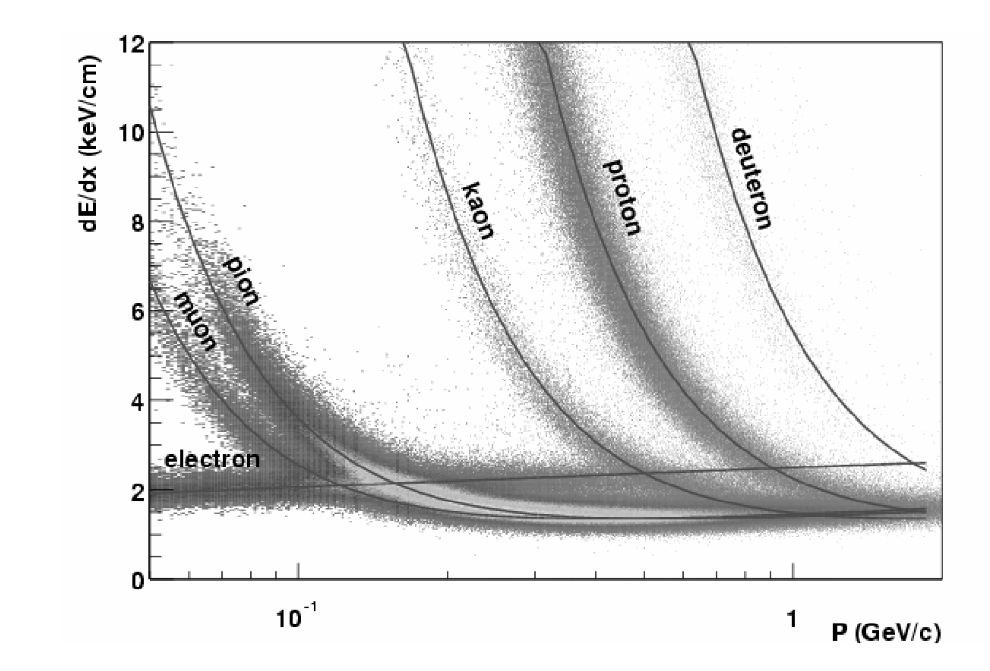
\includegraphics[scale=0.5]{STAR_Detectors/BB_Identification}
	\caption{Κατανομές απώλειας ενέργειας συναρτήσει της ορμής απ' τις οποίες γίνεται η ταυτοποίηση}
	\label{fig3.}
\end{figure}

\section{Barrel Electromagnetic Calorimeter (BEMC)}

	Τα καλορίμετρα αποτελεούν καταστρεπτικούς ανιχνευτές, δηλαδή επιτελούν τις διάφορες διαδικασίες ανίχνευσης εξαναγκάζοντας τα σωματίδια να εναποθέσουν την ενέργειά τους στο υλικό και εν τέλει να σταματήσουν. Άρα στην συνέχεια τα σωματίδια δεν θα είναι διαθέσιμα για περεταίρω μετρήσεις, όπως συμβαίνει για παράδειγμα όταν διέρχονται από έναν TPC, και γι' αυτό τα καλορίμετρα τοποθετούνται συνήθως στα εξωτερικά στώματα των ανιχνευτών. 
	
	Ο STAR έχει δύο ηλεκτρομαγνητικά καλορίμετρα, το Barrel Electromagnetic Calorimeter (BEMC) και το Endcap Electromagnetic Calorimeter (EEMC). Αυτά βασίζονται στο φαινόμενο του ηλεκτρομαγνητικού καταιγισμού, ο οποίος προκαλείται όταν ένα υψηλής ενέργειας ηλεκτρόνιο ή φωτόνιο προσπίπτει σε πυκνό υλικό. Πιό συγκεκριμένα, όταν ένα ηλεκρόνιο ταξιδέψει σε ένα υλικό για μήκος ίσο με το radiaition length $X_0$, τότε θα ακτινοβολήσει σίγουρα ένα φωτόνιο Bremstralhung, ενώ ένα ενεργητικό φωτόνιο έχει περίπου 64\% πιθανότητα να κάνει διδυμη η γέννηση και να παραχθεί ζεύγος $e^-e^+$. Συνεπώς σε $X_0$ έχουμε διπλασιασμό των σωματιδίων και μετά από $\Delta x = t\cdot X_0$ θα έχουμε $n(t) = 2^t$ σωματίδια. 
	
	Η ανάπτυξη του καταιγισμού οδηγεί σε αύξηση του αριθμού δευτερογενών ηλεκτρονίων και φωτονίων επομένως στην μείωση της ενέργειας του καθε νέου σωματιδίου. Για παράδειγμα, αν η ενέργεια του αρχικού σωματιδίου είναι $E_0$, τότε στο πρώτο $X_0$ κάθε νέο σωματίδιο αποκτά ενέργεια $E_0/2$, άρα μετά από $\Delta x = t\cdot X_0$ κάθε σωματίδιο έχει ενέργεια $E(t) = E_0\cdot 2^t$.
	
	Γίνεται αισθητό πως καθώς μειώνεται η ενέργεια των σωματιδίων αυτά δεν θα χάνουν ενέργεια κυρίως με Bremstahlung αν είναι ηλεκτρόνια και δεν θα μπορούν να κάνουν δίδυμη γέννηση αν είναι φωτόνια. Συνεπώς είναι λογικό να υπάρχει μία ενέργεια κάτω από την οποία να μην είναι δυνατή η συνέχιση του καταιγισμού. 
	Αυτή η ενέργεια είναι η κρίσιμη ενέργεια, δηλαδή αυτή στην οποία οι απώλειες του αρχικού ηλεκτρονίου από Bremstrahlung και ιονισμό του υλικού είναι ίσες. Από εκεί και πέρα η ενέργεια των εναπομείναντων σωματιδίων του καταιγισμού χάνεται μέσω ιονισμών και διεγέρσεων του υλικού που διασχίζουν.
	
	Άρα η συνθήκη τερματισμού του Ηλεκτρομαγνητικού Καταιγισμού είναι 
		\begin{equation*}\label{eq3.3}
			E(t_{max}) = E_c \numberthis
		\end{equation*}
	Από την οποία προκύπτει και ο μέγιστος αριθμός γενεών σωματιδίων 
		\begin{equation}\label{eq3.4}
			t_{max} = \frac{lN(E_0/E_c)}{ln(2)}
		\end{equation}
	Ένας τυπικός αριθμός γενεών είναι 20-25 άρα θέλουμε ένα υλικό 20-25$X_0$ προκειμένου να παγιδεύσουμε πλήρως τον Ηλεκτρομαγνητικό Καταιγισμό του αρχικού σωατιδίου άρα και όλη του την ενέργεια.
	
	 Τα παραπάνω ήταν σχετικά με την διαμήκη συμπεριφορά του Καταιγισμού της οποίας τυπικό μήκος είναι το μήκος ακτινοβολίας $X_0$. Η εγκάρσια συμπεριφορά του καθορίζεται από τις πολλαπλές σκεδάσεις Coulomb με τους πυρήνες του υλικού που έχουμε επιλέξει και το χαρακτηριστικό της μήκος είναι η ακτίνα Moliere η οποία ορίζεται ως 
	 \begin{align}\label{eq3.5}
	 	R_M = \frac{(charact. energy)\times X_0}{E_c}
	 \end{align}
	όπου η χαρακτηριστική ενέργεια είναι $\simeq21MeV$. αν είχαμε έναν κύλινδρο απείρου μήκους και ακτίνας $R_M$, τότε αυτός θα περιείχε το 90\% της ενέργειας του καταιγισμού, ενώ αν η ακτίνα του ήταν $2R_M$ θα περιείχε το 95\%.
	
	
	Υπάρχουν καλορίμετρα διαφόρων ειδών που ποικίλουν ως προς τα χαρακτηριστικά  και την διακριτική ικανότητά τους και επιλέγονται ανάλογα με τις ανάγκες του εκάστοτε πειράματος. Το BEMC του STAR, είναι ένα Scintillating Sampling Calorimeter με Μόλυβδο, το οποίο ήταν μία βολική, ευέλικτη και οικονομική επιλογή για να καλύψει τους περιορισμούς που επιβάλλει η γεωμετρία του STAR, όπου θα πρέπει να τοποθετηθεί σε έναν κλειστό χώρο ενδιάμεσα από άλλους ανιχνευτές, συστήματα και εντός μαγνητικού πεδίου. 
	
%	\begin{figure}[h!]
%			\centering 
%			\includegraphics[scale=0.5]{STAR_Detectors/Detectors_Cross_Section.png}
%			\caption{Τομές του STAR όπου φαίνεται η θέση του BEMC}
%			\label{fig3.11}
%		\end{figure}
			
			\begin{figure}[h!]
				\centering
				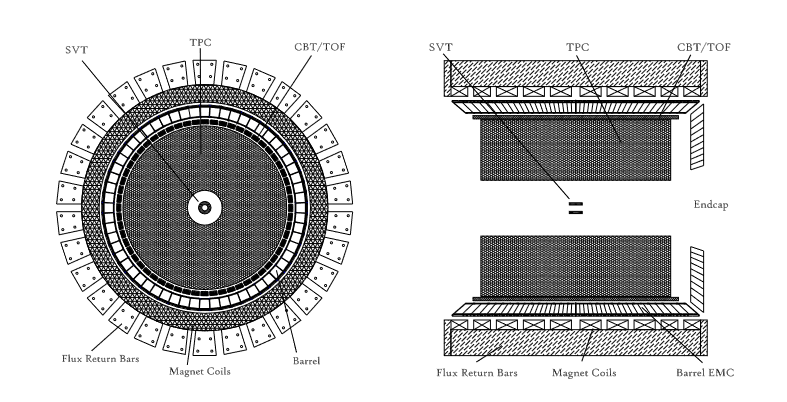
\includegraphics[scale=0.4]{STAR_Detectors/Detectos_Cross_Section}
				\caption{Τομές του STAR όπου φαίνεται η θέση του BEMC}
				\label{fig3.11}
			\end{figure}
	
	
	Ο στόχος του είναι η μελέτη διαδικασιών με υψηλή κάθετη ορμή $p_T$, όπως πίδακες, βαρέα κουάρκ και να παρέχει μεγάλη γεωμετρικη αποδοχή σε πρωτόνια, ηλεκτρόνια, $\pi^0$ και $\eta$ μεσόνια προερχόμενα από κρούσεις πολωμένων πρωτονίων και Au-Au. 
	Καλύπτει μία γεωμετρική περιοχή $60m^2$ για pseudorapidity $|\eta|<1$.
	Για την επίτευξη των στόχων θα πρέπει να είναι σε θέση να εγκλωβίσει ενέργεια καταιγισμού 60GeV και γι' αυτό έχει ακτίνα 20$X_0$.
	
	Ο BEMC κατασκευάζεται από μικρά τμήματα μολύβδου και πλαστικού σπινθηριστή για να είναι ευκολότερη η εγκατάστασή του στο εσωτερικό του STAR. Οι γεωμετρικοί περιορισμοί διευκολύνουν κάποια ζητήματα ενώ ταυτόχρονα δυσκολεύουν άλλα. Για παράδειγμα, τα φωτόνια που παράγονται στον σπινθηριστή οδηγούνται στον φωτοπολλαπλασιαστή και έπειτα στα ηλεκτρονικά που, λόγω περιορισμένου χώρου, θα πρέπει να είναι τοποθετημένα εκτός του κυλινδρικού χώρου του STAR. Αυτό διευκολύνει στο γεγονός ότι  οι φωτοπολλαπλασιαστές είναι τοποθετημένοι εκτός του μαγνητικού πεδίο, άρα δεν αλλοιώνεται το σήμα τους, αλλά ταυτόχρονα περιπλέκει το οπτικό συστημα που θα οδηγήσει τα φωτόνια ως αυτήν την περιοχή.
	
	Για τους στόχους του STAR, θα πρέπει να είναι δυνατή η ανακατσκευή τροχιών $\pi^0$ και απευθείας φωτονίων σε ορμές $p_T=25-30GeV/c$, η ανίχνευση ηλεκτρονίων και ζευγων quark-antiquark σε περιβάλλον με έντονο αδρονικό υπόβαθρο. Για να γίνει αυτό, θα πρέπει να υπάρχει η δυνατότητα ακριβούς ανακατασκευής τροχιών με μεγάλη χωρική διακριτική ικανότητα.
	
	
	Συνολικά αποτελείται από 120 τμήματα (modules) Μολύβδου-Σπινθηριστή πλάτους 26cm και μήκους 293cm. Άρα κάθε τμήμα καλύπτεί γωνίες $\Delta \phi=6^o$ και $0<\eta<1$ (Εικόνα (\ref{fig3.12}a)). Κάθε τμήμα περιέχει 40 "Πύργους" (Towers)	, 2 κατά την $\phi$ και 20 κατά την η διεύθυνση.
	
	Κάθε πύργος περιέχει 20 στρώματα μολύβδου 19mm, 19 στρώματα σπινθηριστή 5mm και 2 στρώματα σπινθηριστή 6mm. Τα πιό παχιά στρώματα σπινθηριστή έχουν τοποθετηθεί στην αρχική περιοχή του ανιχνευτή, δηλαδή πιό κοντά στην δέσμη. Αυτή η περιοχή ονομάζεται Pre-shower Detector και παρέχει ανεξάρτητες μετρήσεις της διαμήκους εξέλιξης του καταιγισμού στα αρχικά στάδια (1-1.5 $X_0$) η οποία βοηθάει στην διάκριση των $\pi^0$ - $\gamma$ και φορτισμένων αδρονίων-ηλεκτρονίων.
	Σε αυτή την περιοχή υπάρχει αισθητή διαφορά στην εναπόθεση ενέργειας μεταξύ των ηλεκτρονίων και φορτισμένων αδρονίων. Ένα ηλεκτρόνιο ιονίζει περισσότερο το υλικό από ένα αδρόνιο ακόμη και πριν από την έναρξη του καταιγισμού ενώ ταυτόχρονα το 60\% των ηλεκτρονίων θα ξεκινήσει τον καταιγισμό πριν την είσοδό του στον Pre-shower σε αντίθεση με το 3\% των αδρονίων. 
	
	\begin{figure}[h!]
    \centering
    \subfloat[\centering Ο BEMC από πλευρική όψη]{{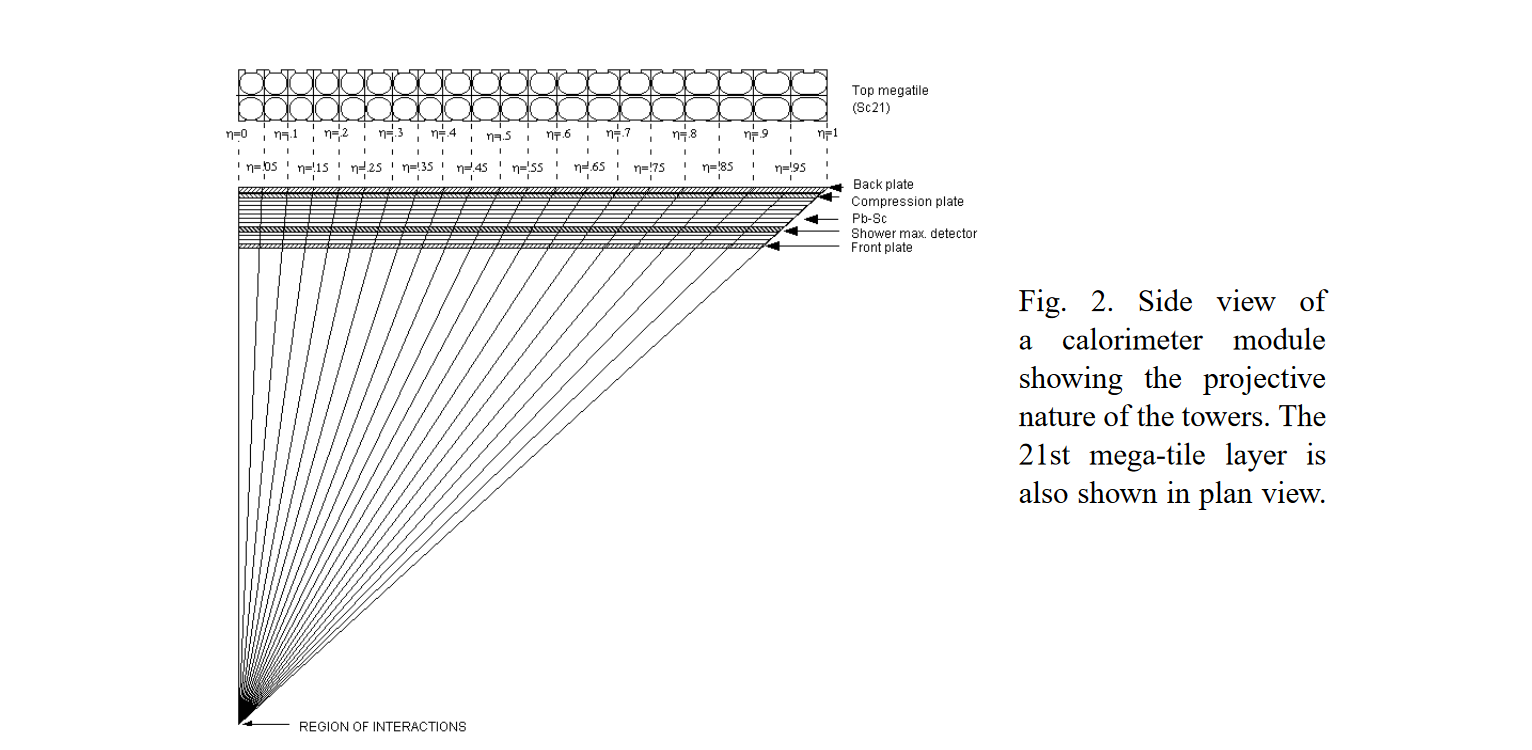
\includegraphics[width=7.5cm]{STAR_Detectors/BEMC_side_view} }}%
    \qquad
    \subfloat[\centering Δομή Μολύβδου-Σπινθηριστή]{{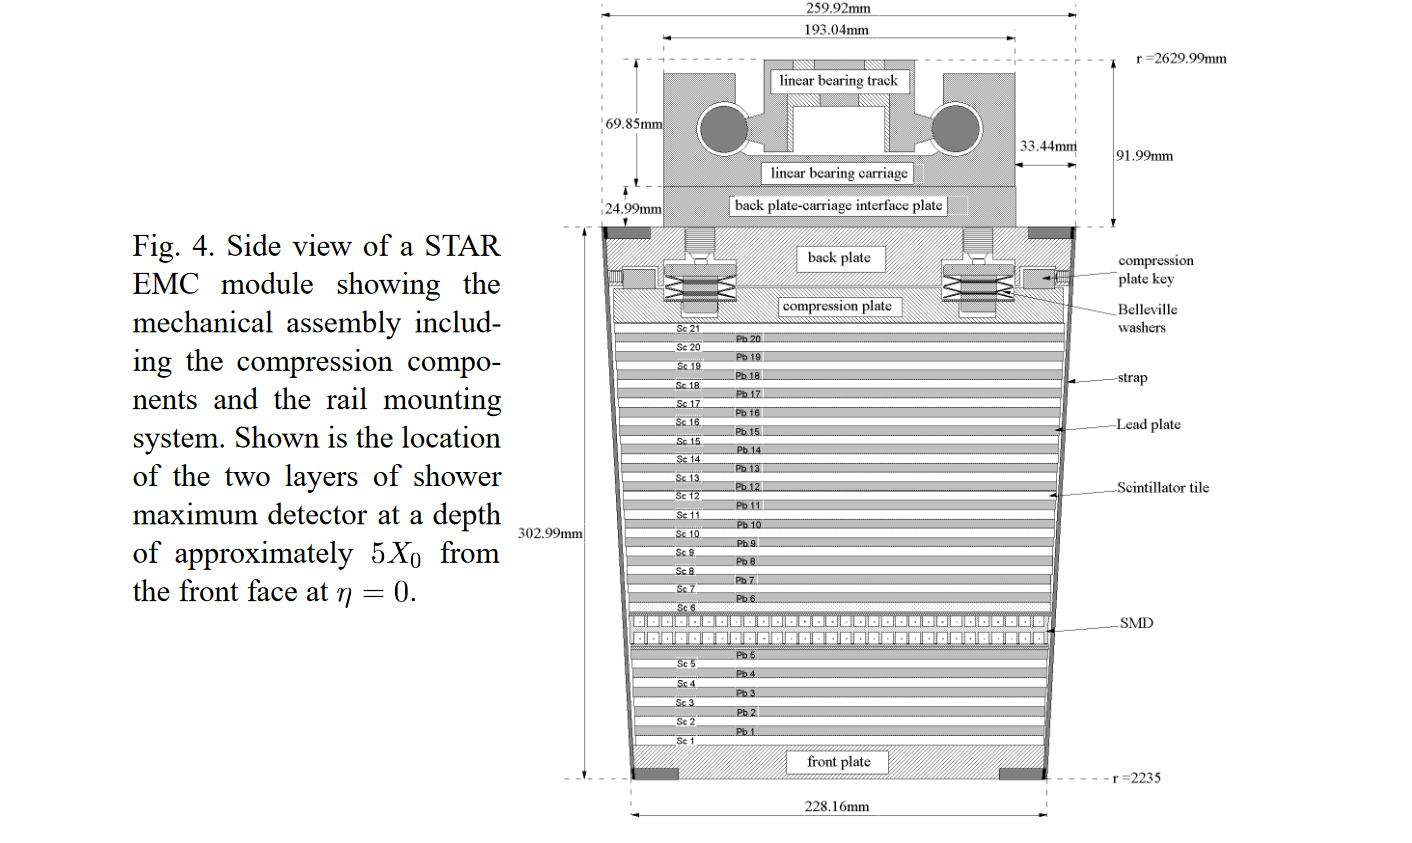
\includegraphics[width=7.5cm]{STAR_Detectors/BEMC_side_view2} }}%
    \caption{Πλευρικές όψεις του ΒΕΜC}
    \label{fig3.12}%
\end{figure}

	Τα 21 στρώματα σπινθηριστή του κάθε στρώματος είναι σε μορφή 40 ορθογωνίων παραλληλεπιπέδων εκ των οποίων τα 2 καλύπτουν γωνία $\phi$ και τα 20 $\eta$ όπως φαίνεται στην Εικόνα (\ref{fig3.12}b). Αυτοί είναι οπτικά απομονωμένοι και συνδέονται με μία οπτική ίνα, η οποία έχει καθορισμένη θέση εντός του στρώματος και μεταφέρει το σήμα στους φωτοπολλαπλασιαστές
	
	Τέλος, σε απόσταση περίπου 5.6$X_0$ από την αρχή του ανιχνευτή είναι εκεί όπου επιτυγχάνεται το μέγιστο της ενέργειας του καταιγισμού. Εκεί, διακόπτεται τοπικά η διαδοχή μολύβδού-σπινθηριστή και παρεμβάλλεται ένας αναλογικός ανιχνευτής αερίου (Shower Maximum Detector - SMD).
	Αυτός, επιτελεί τον σκοπό της βελτίωση της διαμήκους χωρικής διακριτικής ικανότητας που βοηθά στην ανακατσκευή των $\pi^0$, την ταυτοποίηση γ και e.
	
	O SMD αποτελείται από 50μm επιχρυσωμένα σύρματα βολφραμίου που είναι τοποθετημένα απέναντι από τμήματα καθόδου τα οποία ανιχνεύουν την αυξημένη συγκέντρωση φορτίου γύρω από τα σύρματα. To στοιχείο που βελτιώνει την απόδοσή του είναι πως υπάρχουν αντικριστά δύο επίπεδα από ανόδους-καθόδους, ένα πιό κοντά στην δέσμη και ένα πιό μακριά.
	
\section{Endcap Electromagnetic Calorimeter (EEMC)}

	Το Endcap Electromagnetic Calorimeter (EEMC) παρέχει κάλυψη σε γωνία $\Delta\phi=2\pi$ και $1.086<\eta<2.000$ για υψηλής $p_T$ φωτόνια, ηλεκτρόνια και διασπώμενα μεσόνια. 
	Όπως και το BEMP περιέχει έναν SMD (Shower Maximum Detector) για διάκριση των $\pi^0/\gamma$, preshower-postshower στρώματα για την διάκριση ηλεκτρονίων - φορτισμένων αδρονίων. Η συνεισφορά του είναι μεγαλύτερη στο πρόγραμμα για τα πολωμένα πρωτόνιο παρά για τα φορτισμένα ιόντα. Εκεί ένας σημαντικός στόχος είναι ο προσδιορισμός της προτιμώμενης ελικότητας των γλουονίων εντός ενός πολωμένου πρωτονίου σαν συνάρτηση του ποσοστού της ορμής ($x_g$) που κατέχει. Επίσης, στόχος του προγράμματος πολωμένων πρωτονίων είναι η συνολική συνεισφορά του σπιν των γλουονίων στο σπιν του πρωτονίου.
	Η πόλωση των γλουονίων μπορεί να ανιχνευτεί σε σκεδάσεις Compton κουαρκ-γλουονίων, μετρώντας τις διαμήκεις συσχετίσεις σπιν. 
	Ακόμη, το EEMC θα βελτιώσει την ευαισθησία του STAR στην εξάρτηση της γεύσης της πόλωσης των τελικών κουάρκ μέσω της παραγωγής $W^{\pm}$.	
	H εστίαση στις κρούσεις p-p συνεπάγεται πως ειναι δυνατή η μείωση των αριθμών των ξεχωριστών κομματιών, σε αντίθεση με το BEMC που εστίαζε στις κρούσεις Au-Au που παράγουν πολλά σωματίδια, άρα η μεγαλύτερη διαμέρισή του ήταν πιό αναγκαία.  
	
	Ομοίως με το BEMC, το εν λόγω καλορίμετρο αποτελείται από διαδοχικά στρώματα μολύβδου-πλαστικού σπινθηριστή (23 και 24 αντίστοιχα) που επιλέχθηκαν λόγω χαμηλού κόστους. Συνολικά καλύπτει περίπου 21.4$X_0$ και λιγότερο από ένα interaction length $\lambda$.
	Οπτικές ίνες συνδέουν τις μονωμένες από φως περιοχές του σπινθηριστή με τους φωτοπολλαπλασιαστές που βρίσκονται και πάλι εκτός της περιοχής ανίχνευσης.
	
	Ο SMD τοποθετείται μετά το πέμπτος ζεύγος μολύβδου-σπινθηριστή και είναι χρήσιμος για την διάκριση μεταξύ ηλεκτρονίων/αδρονίων καθώς και την αντιστοίχιστη των $e^\pm$ με εκείνα που ανιχνεύονται στον TPC. Εδώ δεν πρόκειται για θάλαμο αερίου αλλά αποτελείται και αυτός απο σπινθηριστή που παράγει ένα οπτικό σήμα οδηγούμενο προς τους φωτοπολλαπλασιαστές.
	
	Υπάρχει επίσης και ο pre-shower ανιχνευτής. Αυτός δεν είναι τίποτα άλλο από τα δύο πρώτα στρώματα σπινθηριστή που έχουν συνδεθεί με ξεχωριστή οπτική ίνα. Το οπτικό σήμα αυτών προστίθεται στο σήμα των υπολοίπων σπινθηριστών, ενώ το σήμα από τον δεύτερο καταγραφεται και ξεχωριστά. Έτσι, συγκρίνοντας αυτά τα σήματα με το συνολικό σήμα ενός "πύργου" (δηλαδή μία στοίβας από κάθετα τοποθετημένους σπινθηριστές) μπροούμε να ξεχωρίσουμε τα ηλεκτρόνια από τα αδρόνια εκμεταλλευόμενοι τις διαφορές στην πιθανότητα δημιουργίας καταιγισμού.
	Έπίσης, βελτιώνουν την ικανότητα διάκρισης μεταξύ $\pi^0/\gamma$ καθώς η πιθανότητα ένα ενεργητικό φωτόνιο να αφήσει ενέργεια σε αυτά τα στρώματα είναι διπλάσια.
	
	

\section{Silicon Vertex Tracker (SVT)}

Ο Silicon Vertex Tracker (SVT) είναι ένα σύστημα που βασίζεται σε τρία στώματα από Silicon Drift Detectors (SDDs) και μπορεί να δώσει διδιάστατες ανιχνεύσεις με ανιχνευτική ικανότητα της τάξης των 20μm σε κάθε διέυθυνση. Ακόμη, συνεισφέρει στην ταυτοποίηση των σωματιδίων καθώς παρέχει επίσης καλή διακριτική ικανότητα στις μετρήσεις απωλειών ενέργειας. 
	Πέρα από αυτές τις συνεισφορές, οι οποίες βελτιώνουν διαδικασίες που πραγματοποιούνται και από άλλα όργανα του STAR, ο SVT προσδίδει μία επιπλέον δυνατότητα ανίχνευσης που δεν προσφέρουν οι υπόλοιποι ανιχνευτές.
	Δεδομένου ότι είναι ο πιο κοντινός ανιχνευτής στην δέσμη (Εικόνα \ref{fig3.2}), μπορεί να ανακατασκευάζει τροχιές από σωματίδια με πολύ μικρό χρόνο ζωής, όπως  D-μεσόνια και strange \& mulitystrange βαρυόνια τα οποία αναμένεται να υπάρχουν σε αφθονία στο Quark Gluon Plasma.
	Ακόμη, επεκτείνει την αποδοχή του ανιχνευτή και σε σωματίδια με πολύ χαμηλή ορμή τα οποία λόγω του μαγνητικού πεδίου δεν προλαβαίνουν να φτάσουν στον TPC.


%%%%%%%%%%%%%%%%%%%%%%%%%%55
%%% na valw to label
%	\begin{figure}[h!]
%		\centering 
%		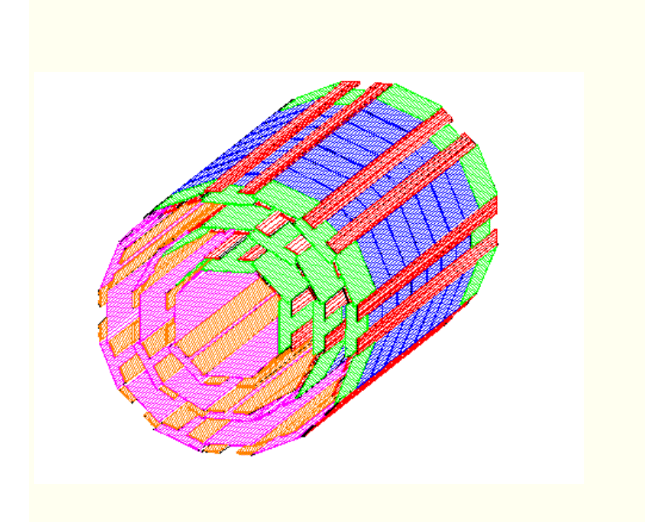
\includegraphics[scale=0.5]{STAR_Detectors/SVD_3_Layers}
%		\caption{Τα τρία στρώματα από SDD του SVT}
%		\label{fig3.13}
%	\end{figure}
	
	\begin{figure}[h!]
    \centering
    \subfloat[\centering Τα τρία στρώματα από SDD του SVT]{{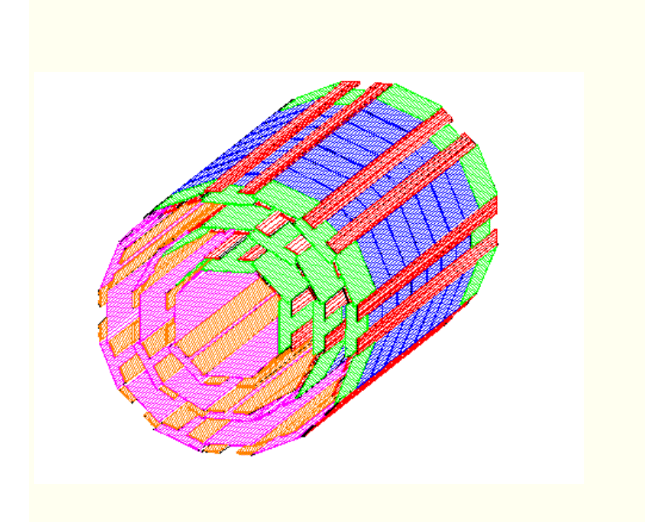
\includegraphics[width=7cm]{STAR_Detectors/SVD_3_Layers} }}%
    \qquad
    \subfloat[\centering Φωτογραφία του SVT            ]{{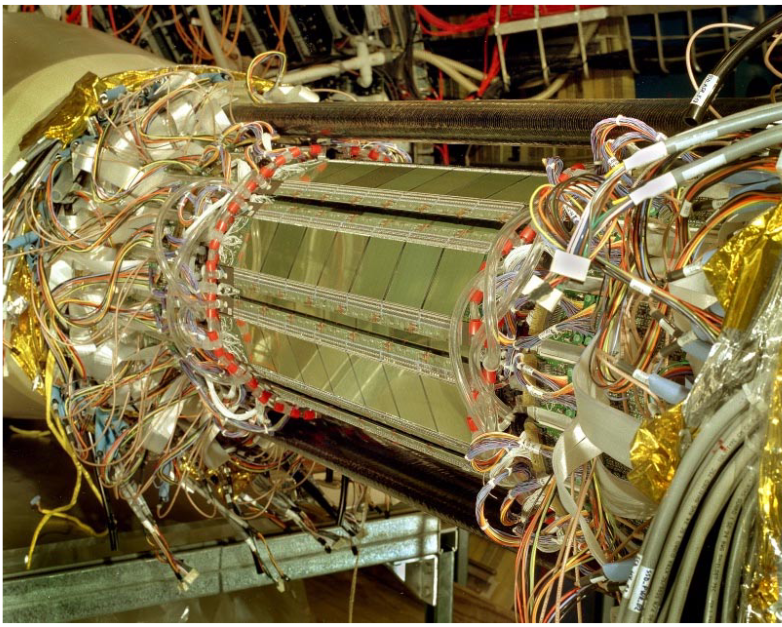
\includegraphics[width=7cm]{STAR_Detectors/SVD_photo} }}
    \caption{Η δομή του SVT}%
    \label{fig3.13}%
\end{figure}	
	
	
	Ο SVT αποτελείται από τρία στώματα Silicon Drift Detectors (SDD). Το κάθε στρώμα αποτλείται από 8,12,16 ράβδους στήριξης οι οποίες τοποθετούνται περιμετρικά της δέσμης και η κάθε ράβδος συγκρατεί 4, 6, 7 τμήματα SDD αντίστοιχα σε κάθε στρώμα, άρα συνολικά υπάρχουν 216 τμήματα SDD. Τα στρώματα είναι σε ακτίνες 5.9cm, 10.2cm, 14.9cm από την δέσμη και το συνολικό μήκος είναι 44.1cm. Ο μεγάλος αριθμός από ανιχνευτικά τμήματα σε τόσο μικρό χώρο είναι αναγκαίος διότι εκεί θα υπάρχουν οι μεγαλύτερες συγκεντώσεις φορτισμένων σωματιδίων, περιπου 1500-3000 ανά γεγονός. 
	
	Ας δούμε τώρα τι ακριβώς είναι οι SDD. Θα μπορούσαμε να τους φανταστούμε ως  κάτι σαν Time Projection Chambers αλλά στερεάς κατάστασης. Ο πιό απλός τέτοιου τύπου ανιχνευτής στερεάς κατάστασης θα αποτελούταν από μία επίπεδη επαφή p-n από Si. Αν φέρουμε σε επαφή έναν ημιαγωγό τύπου p και έναν n, τότε οι οπές του p και τα ηλεκτρόνια του n κινούνται λόγω διάχυσης προς αντίθετες κατευθύνσεις, γεννώντας ένα ρεύμα διάχυσης $I_0$. Κατά την κίνησή τους επανασυνδέονται και δημιουργείται μία περιοχή απογύμνωσης. 
	Αυτή η περιοχή, δεδομένου ότι από τον n έχουν απομακρυνθεί κάποια ηλεκτρόνια, γίνεται θετικά φορτισμένη με οπές από την μερία του n και αντίστοιχα αρνητικά φορτισμένη με ηλεκτρόνια από την μεριά του p. Έτσι, δημιουργείται και ένα ηλεκτρικό πεδίο από την n στην p. Αυτό το πεδίο αντιστέκεται στην διάχυση των φορέων και εν τέλει επιτυγχάνεται μία κατάσταση ισορροπίας στην οποία μηδενίζεται το ρεύμα.
	
	 Εφαρμόζοντας τώρα διαφορά δυναμικού μεταβάλλουμε το πλάτος της περιοχής απογύμνωσης, το ηλεκτρικό πεδίο εντός αυτής και κατ' επέκταση το ρεύμα θα δίνεται από την σχέση 
	 \begin{align}\label{eq3.6}
	 	I = I_0 (exp(\frac{qV}{kT})-1) 
	 \end{align}
%	και η αντίστοιχη αντίσταση που δημιουργείται από την 
%	\begin{align}\label{eq3.7}
%		R_F = \left( \odv{I}{V}\right)^{-1} = \frac{kT}{qI}
%	\end{align}
	Όπως έχει ήδη αναφερθεί, στην κατάσταση ισορροπίας και χωρίς εξωτερική τάση, V=0, το ρεύμα μηδενίζεται. Αν εφαρμόσουμε ορθή πόλωση ($V>0$) δηλαδή μεγαλύτερο δυναμικό στην p περιοχή, μικραίνουμε το μήκος της περιοχής απογύμνωσης και τότε ηλεκτρόνια και οπές χρειάζονται μικρότερη ενέργεια για να μεταπηδήσουν το φράγμα δυναμικού και να πάνε στην άλλη περιοχή άρα το ρεύμα αυξάνεται. Αυτό υποδεικνύει και η εξίσωση (\ref{eq3.6}). 
	Αντιθέτως, αν εφαρμόσουμε ανάστροφη πόλωση, $V<0$, τότε το ρεύμα μειώνεται και η περιοχή απογύμνωσης μεγαλώνει καθώς τα αρνητικά φορτία του n ημιαγωγού κατευθύνονται στην περιοχή θετικής τάσης που εφαρμόζεται στην άκρη του και αντίστοιχα οι θετικές οπές του p κατευθύνονται προς την περιοχή αρνητικής τάσης που εφαρμόζεται στην άκρη του.
	
	Εμείς θέλουμε να εκμεταλλευτούμε τις ιδιότητες μίας επαφής p-n προκειμένου να κατασκευάσουμε έναν ανιχνευτή. Η ιδέα είναι ότι όταν ένα φωτόνιο ή ένα φορτισμένο σωματίδιο εισέλθει στην περιοχή απογύμνωσης, ενδέχεται να αλληληπιδράσει με τον Si και να δημιουργήσει εξτρα ζεύγος ηλεκτρονίου-οπής τα οποία θα οδηγηθούν σε αντίθετες κατευθύνσεις εξαιτίας του πεδίου και θα συλλεχθούν στα άκρα των περιοχών p, n από ηλεκτρόδια. Συγκεκριμένα, ένα φωτόνιο θα δημιουργήσει μόνο ένα ζεύγος, ενώ ένα φορτισμένο σωματίδιο αναμένουμε να δημιουργήσει ζεύγη κατά μήκος της τροχιάς.
	 
	 Εμείς θέλουμε να κατασκευάσουμε μία κατάσταση στην οποία το ρεύμα λόγω διάχυσης θα είναι μικρό σε σύγκριση με το ρεύμα που δημιουργείται από τις αλληλεπιδράσεις, επομένως αυτά να μπορούν να διαχωριστούν. Άρα θα χρησιμοποιήσουμε ανάστροφη πόλωση. Η ανάστροφη πόλωση μεγαλώνει την περιοχή απογύμνωσης, δηλαδή την περιοχή στην οποία θα γίνουν οι αλληλεπιδράσεις με τα σωματίδια που θέλουμε να ανιχνεύσουμε.
	Όταν αυξήσουμε αρκετά την διαφορά δυναμικού, τότε φτάνει σε μία τιμή $V_D$, στην οποία η απογύμνωση είναι πλήρης και όλοι οι φορείς έχουν απομακρυνθεί στις διόδους αφήνοντάς την ουδέτερα φορτισμένη.	
	%
	Μία τέτοια δίοδος που  έχει φορείς υψηλής κινητικότητας και μικρό όγκο,  είναι κατάλληλη για να τοποθετηθεί ως ανιχνευτής σε περιοχές υψηλής ροής σωματιδίων, όπως εκεί που τοποθετείται στο STAR.
	
	Η ιδέα συγκεκριμένα για τους SDD πηγάζει από την απλή δίοδο όπως αυτή που περιγράφηκε φτιαγμένη από Si. 
	Γενικά, δεν φέρνουμε ακριβώς σε επαφή τους n \& p ημιαγωγούς αλλά παρεμβάλλουμε μεταξύ τους κάποιον άλλον ημιαγωγό, με πολύ χαμηλότερη συγκέντρωση προσμίξεων, στην περιοχή του οποίου δημιουργούνται τα ζεύγη ηλεκτρονίων-οπών από τα σωματίδια. 
	Η πιό απλή περίπτωση είναι να έχουμε έναν κύριο όγκο από τέτοιο υλικό και κατά μήκος δύο απέναντι πλευρών του να τοποθετήσουμε την άνοδο (n ημιαγωγός) και την κάθοδο (p ημιαγωγός) όπου θα μαζεύονται τα ζεύγη ηλεκτρονίων-οπών που θα δημιουργούν τα προς ανίχνευση σωματίδια.
	Ωστόσο, αυτό μπορεί να λειτουργήσει ακόμη και όταν οι παραπάνω ημιαγωγοί δεν καλύπτουν πλήρως τα άκρα της διόδου όπως φαίνεται στην Εικόνα (\ref{fig3.14}a).
	Τότε δημιουργείται επιπλέον χώρος και μπορούμε  πάρουμε τον n από την μία πλευρά του κύριου όγκου και να τον τοποθετήσουμε δίπλα από τον p, χωρίς βέβαια να ακουμπάνε (Εικόνα (\ref{fig3.14}b). Έτσι αφήνουμ χώρο για έναν ακόμη p ημιαγωγό στην κάτω πλευρά του Si. 
	Τότε, σε χαμηλές τάσεις δημιουργούνται δύο φορτισμένες περιοχές γύρω από τους p εντός του Si oι οποίες διαχωρίζονται από μία ουδέτερη ζώνη (Εικόνα \ref{fig3.15}c). Για μεγαλύτερη διαφορά δυναμικού το πλάτος της ουδέτερης περιοχής μειώνεται και συγκεντρώνεται γύρω από τον n ημιαγωγό, ενώ οι δύο φορτισμένες περιοχές θα έχουν κοινό όριο και στο εσωτερικό τους θα υπάρχουν αντίθετα πεδία που κατευθύνονται προς τους ημιαγωγούς p (Εικόνα (\ref{fig3.14}d).
	Δημιουργείται έτσι μία περιοχή στην οποία τα ηλεκτρόνια έλκονται μόνο από την άνοδο, τον ημιαγωγό n και οι αντίστοιχες οπές κατευθύνονται ταχύτατα προς τις καθόδους, τους ημιαγωγούς p.
	Αν τώρα τοποθετήσουμε επιπλέον ηλεκτρόδια μπορούμε να βελτιώσουμε την ολίσθηση ηλεκτρονίων και οπών εντός του κύριου ημιαγώγιμου υλικού προς τα ηλεκτρόδια (Εικόνα (\ref{fig3.15})).
	%Δημιουργείται έτσι ένα πλατώ δυναμικού για τα ηλεκτρόνια στο οποίο κινούνται μόνο με διάχυση εως ότου φτάσουν στην περιοχή όπου θα έλκονται από την άνοδο. 
	%Ακόμη, για να βοηθηθεί η κίνηση των ηλεκτρονίων προς την άνοδο, τοποθετούμε επιπλέον εξωτερικό ηλεκτρικό πεδίο. 
%	\begin{figure}[h!]
%		\centering 
%		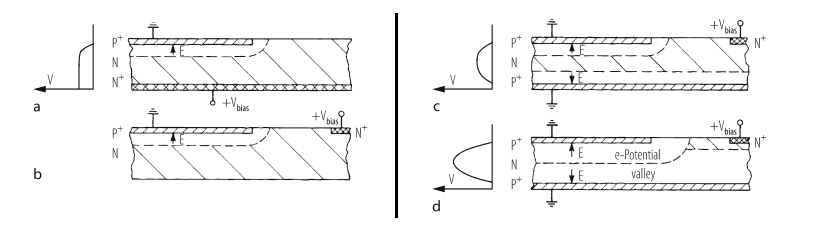
\includegraphics[scale=0.7]{STAR_Detectors/SDD}
%		\caption{Η ιδέα πίσω από τους SDD}
%		\label{fig3.14}
%	\end{figure}	
	\begin{figure}[h!]
    \centering
    \begin{minipage}{.5\textwidth}
        \centering
        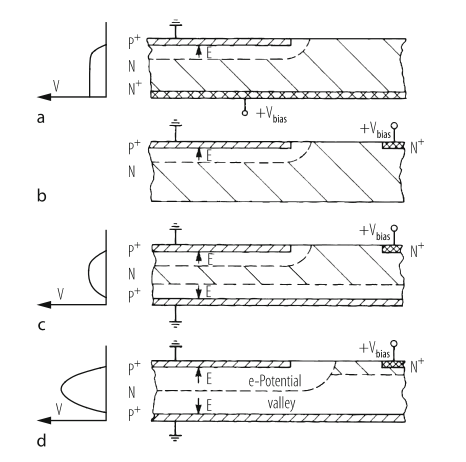
\includegraphics[scale=0.6]{STAR_Detectors/SDD_v}
        \caption{Αρχή Λειτουργίας ενός SDD}
        \label{fig3.14}
    \end{minipage}%
    \begin{minipage}{0.5\textwidth}
        \centering
        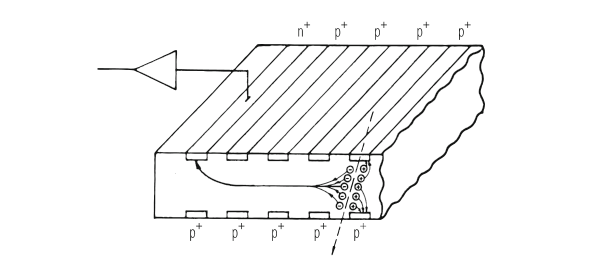
\includegraphics[scale=0.7]{STAR_Detectors/SDD_2}
        \caption{Τελικός SDD με όλες τις ανόδους/καθόδους}
        \label{fig3.15}
    \end{minipage}
\end{figure}
	
	Ο κάθε SDD του STAR έχει πάχος 280μm και καλύπτει μία επιφάνεια 63mm$\times$63mm. Οι άνοδοι τοποθετούνται σε βάθος 250μm και έχουν διαστάσεις 200μm$\times$200μm οι οποίες είναι βολικές για την καταγραφή σημάτων από ηλεκτρόνια των οποίων η διάχυση εντός του Si διαρκεί $\sim \mu sec$ και αποκτά πλάτος $\sim 100\mu m$ σε συνολική απόσταση $\sim 3cm$. 

	%Ένα σημαντικό σημείο είναι να επιτευγχθεί η βέλιτιστη διακριτική ικανότητα στην διεύθυνση ολίσθησης. Για κάτι τέτοιο απαιτείται η ταχύτηα ολίσθησης των παραγόμενων ηλεκτρονίων να είναι γραμμική προς το πεδίο $u_{dr} = \mu_e E$. Ακόμη, θα πρέπει να είναι  γνωστή η λειτουργία των ανιχνευτών 
	%με μεγάλη ακρίβεια η θέση των ανιχνευτών. Συνεπώς, πρωτού την κανονική τους λειτουργία γίνεται η χαρτογράφησή τους κάτω από παρόμοιες συνθήκες. Έτσι, όταν πραγματοποιούνται τα πειράματα μπορούν να 
		
	Η άνοδος στην οποία παράγεται το εκάστοτε σήμα από ηλεκτρόνια, καθώς και ο χρόνος ολίσθησης καθορίζουν τις συντεταγμένες της τροχιάς, ενώ ταυτόχρονα μετρήσεις της απώλειας ενέργειας $dE/dx$, δίνουν ταυτοποιήση των σωματιδίων (Εικόνα (\ref{fig3.1}) 
	
	\begin{figure}[h!]
		\centering 
		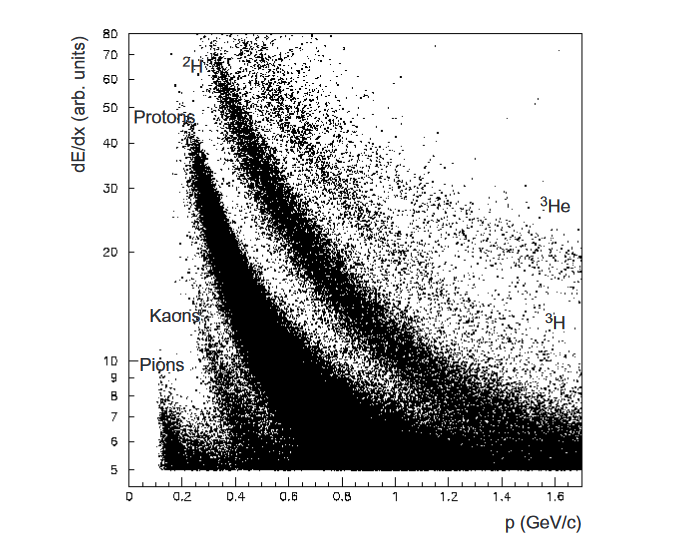
\includegraphics[scale=0.5]{STAR_Detectors/SDD_dedx}
		\caption{Μετρήσεις απώλειας ενέργειας dE/dx σε συγκρούσεις Au-Au 11.6GeV/n στο AGS}
		\label{fig3.}
	\end{figure}
	
	
	
\section{Silicon Strip Detector (SSD)}

O Silicon Strip Detector πρόκειται για ένα τέταρτο στρώμα ανιχνευτών που συμπληρώνουν τα τρια του SVT φτιάχνοντας έτσι ένα σύστημα ιχνηλάτησης των τροχιών εντός του TPC.
	Παρέχει διδιάστατη απεικόνιση των δευτερευοντων σωματιδίων, προεκτείνοντας τις ανακατασκευαστική τροχιών από τον SVT, ενώ ταυτόχρονα κάνει και μετρήσεις απώλειας ενέργειας. Επίσης, βελτιώνει την αποδοτικότητα ανίχνευσης τροχιών στην κεντρικη περιοχή και για σωματίδια χαμληής ορμής.
	Είναι τοποθετημένος μόλις 230mm από την δέσμη και καλύπτει μία περιοχή pseudorapidity $|\eta|<1.2$ για την οποία χρειάζεται συνολική επιφάνεια Si 1$m^2$.
		
	
		\begin{figure}[h!]
    \centering
    \begin{minipage}{.5\textwidth}
        \centering
        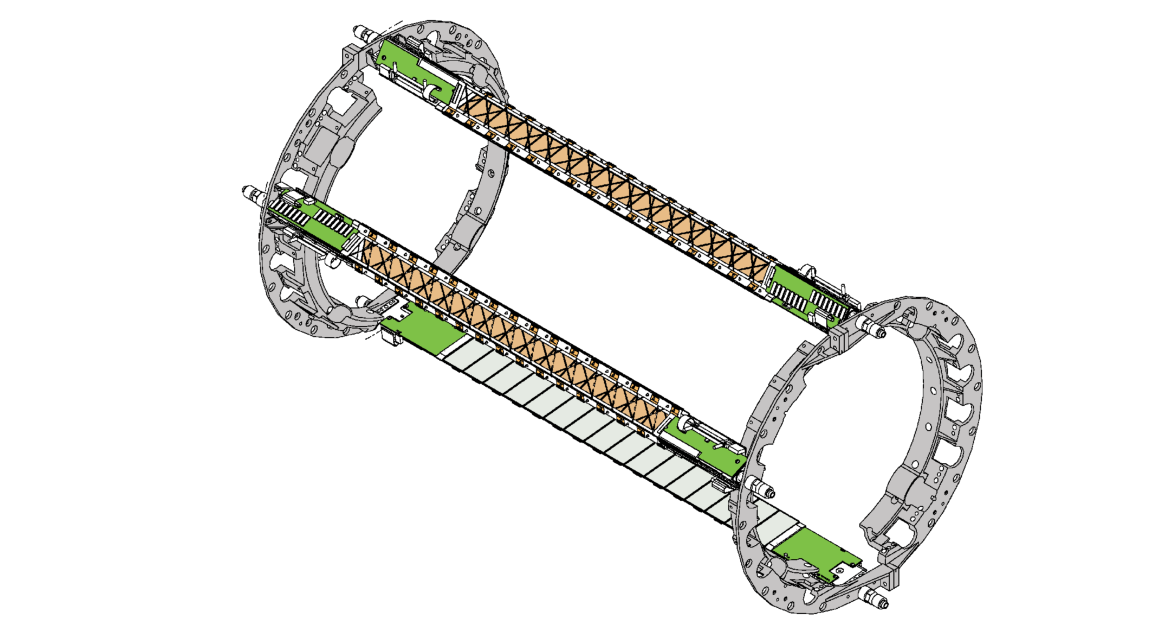
\includegraphics[width=0.9\linewidth, height=0.25\textheight]{STAR_Detectors/SSD_full}
        \caption{Ο SSD με 3 από τις 20 ράβδους}
        \label{fig3.16}
    \end{minipage}%
    \begin{minipage}{0.5\textwidth}
        \centering
        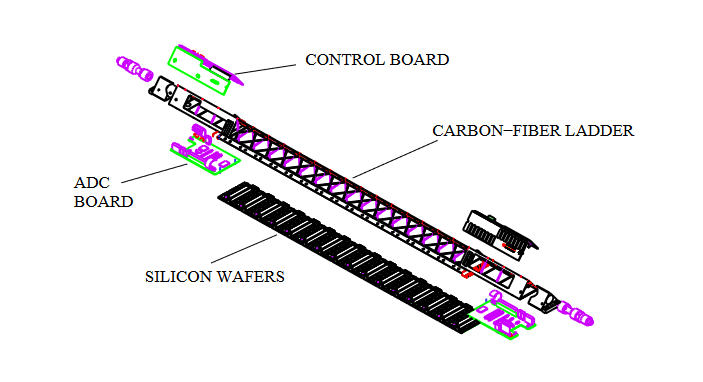
\includegraphics[width=0.9\linewidth, height=0.25\textheight]{STAR_Detectors/SSD_ladder}
        \caption{Η δομή μίας ράβδου του SSD}
        \label{fig3.17}
    \end{minipage}
\end{figure}

	Αποτελείται από 2 ημικυλινδρικά μέρη το κάθενα εκ των οποίων έχει 10 ράβδους. Η κάθε ράβδος στηρίζει 16 τμήματα ανιχνευτών μονάδων απο Πυρίτιο με πάχος 300μm. Η κάθε μονάδα αποτελείται από Πυρίτιο στον κύριο όγκο της, το οποίο είναι και το μέσο στο οποίο γίνονται οι αλληλεπιδράσεις των πρωτεύοντων σωματιδίων και παράγονται τα δευτερεύοντα τα οποία και ανιχνεύουμε. Στις άκρες του κύριου όγκου υπάρχουν λωρίδες διόδων στις οποίες συγκεντώνονται οι φορείς λόγω διάχυσης η οποία προσανατολίζεται από το ηλεκτρικό πεδίο που υπάρχει λόγω των διόδων. Αν τοποθετήσουμε λωρίδες και από τις δύο πλευρές, τότε  καταγράφουμε διπλάσια πληροφορία για το εσωτερικό του ανιχνευτή, συνεπώς έχουμε καλύτερη διακριτική ικανότητα. 
	
	
	
	\begin{figure}[h!]
	    \centering
	    \begin{minipage}{.5\textwidth}
	        \centering
	        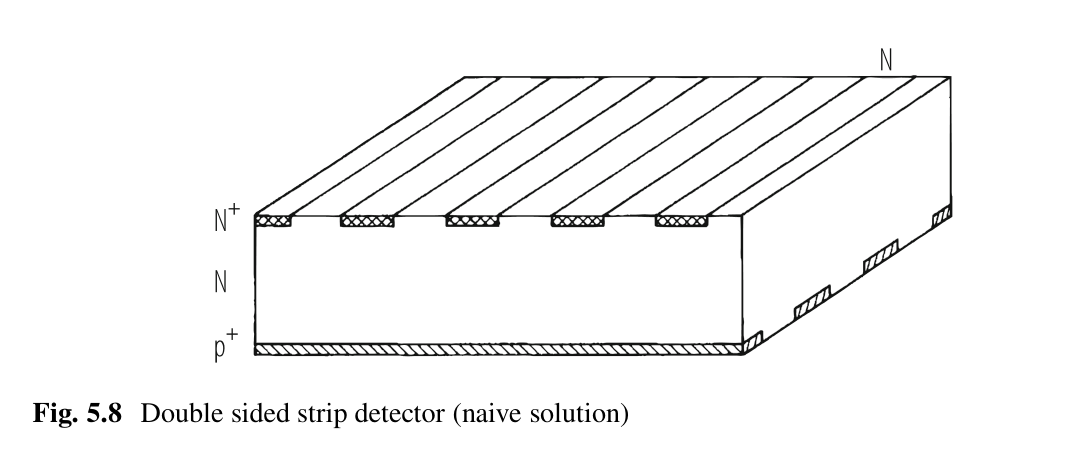
\includegraphics[width=0.9\linewidth, height=0.25\textheight]{STAR_Detectors/SSD_naive}
	        \caption{Μία απλή εκδοχή μίας μονάδας SSD}
	        \label{fig3.19}
	    \end{minipage}%
	    \begin{minipage}{0.5\textwidth}
	        \centering
	        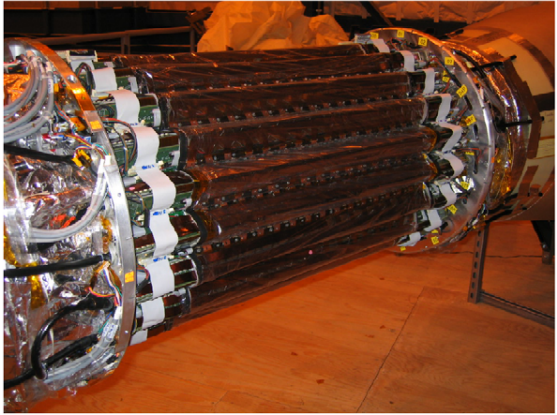
\includegraphics[width=0.9\linewidth, height=0.25\textheight]{STAR_Detectors/SSD_image}
	        \caption{Εικόνα του SSD πριν την εγκατάσταση στο STAR}
	        \label{fig3.20}
	    \end{minipage}
	\end{figure}
	
 	Ένα από τα προβλήματα που προκύπτουν σε έναν τέτοιο ανιχνευτή είναι ότι συσσωρεύονται πολλά ηλεκτρόνια τριγύρω από τις λωρίδες ημιαγωγού τύπου n. για να λύσουμε αυτό το πρόβλημα μπορούμε να εμφυτέψουμε ημιαγωγό τύπου p ενδιάμεσα από τις λωρίδες τύπου n και τότε απομακρύνονται ευκολότερα από την ενδιάμεση περιοχή προς τις διόδους.
 	 
	
\section{Ring Imagning Cherenkov Detector (RICH)}

	Ο ρόλος που επιτελεί ο ανιχνευτής Ring Imaging Cherenkov Detector (RICH) είναι να βελτιώνει την δυνατότητα του STAR για ταυτοποιήση φορτισμένων αδρονίων σε περιοχή μέσης rapidity. Η rapidity ορίζεται ως 
	\begin{align}\label{eq3.7}
		w := arctanh(\frac{u}{ψ})  = \frac{1}{2}ln\frac{e+|\bm{P}|c}{E-|\bm{p}|c}    =\frac{1}{2} ln\frac{E+p_z c}{E-p_zc}
	\end{align}
	όπου z είναι η κατεύθυνση της δέσμης. Συνεπώς στοχεύει σε περιοχές μέσης ορμής. Συγκεκριμένα, στοχεύει σε ανίχνευση καονίων και πιονίων εως 3GeV/c και πρωτονίων εως 5GeV/c μέσω της μέτρησης της μάζας τους και κατ' αυτόν τον τρόπο διευρύνει την ικανότητα ταυτοποίησης των TPC, SVT που εστιάζουν σε σωματίδια χαμηλής ορμής 0.6GeV/c και 1GeV/c αντίστοιχα. Έχει εγκατασταθεί στο κέντρο του ανιχνευτή, άρα καλύπτει περιοχή pseudorapidity $|\eta|<0.3$ και $\Delta\phi=20^o$.
	Οι RICH βασίζονται στην καταγραφή της ακτινοβολίας Cherenkov. Ας δούμε εν συντομία την αρχή με βάση την οποία αυτή λειτουργεί. 
	
	 
	 
	 Γνωρίζουμε πως ένα κινούμενο σωματίδιο εντός ενός υλικού εκπέμπει ακτινοβολία πέδησης η οποία πηγάζει από την αλληλεπίδρασή του με τα άτομα του υλικού και δεν έχει καμία σχέση με την ακτινοβολία Cherenkov. 
	Yπό ορισμένες συνθήκες, εκπέμπεται και μία ακτινοβολία εντλώς διαφορετικής φύσεως, η Cherenkov. Αυτή πηγάζει από το μέσο το οποίο βρίσκεται υπό την επίδραση του πεδίου του κινούμενου σωματιδίου.
	Έστω ότι ένα Η/Μ κύμα διαδίδεται σε ένα διάφανο, ισοτροπικό και μη μαγνητικό διηλεκτρικό μέσο. Τότε η συχνότητά του σχετίζεται με το κυματάνυσμά 
		\begin{align*}\label{eq3.8}
			k = \frac{n(\omega)\omega}{c} = \frac{\sqrt{\epsilon(\omega)} \omega }{c} \numberthis
		\end{align*}
	Επίσης, από τις εξισώσεις Maxwell , υπό την βαθμίδα Lorentz, εντός ενός διηλεκτρικού και αναπτύσσοντας τα δυναμικά σε ολοκληρώματα Fourier, προκύπτει πως η συνιστώσα του κυματανύσματος της ακτινοβολίας στην διεύθυνση που κινείται το σωματίδιο, σχετίζεται άμεσα με την ταχύτητα κίνησης του σωματιδίου. Συγκεκριμένα, αν το σωματίδιο κινείται στον άξονα x, τότε
		\begin{align*}\label{eq3.9}
			k_x = \frac{\omega}{u} \numberthis
		\end{align*}
	Προκειμένου οι εξισώσεις (\ref{eq3.8}) \& (\ref{eq3.9})  να είναι αυτοσυνεπείς, θα πρέπει να ισχύει 
	\begin{align*}\label{eq3.10}
		k_x              <& k \Rightarrow\\
		\frac{\omega}{u} <& \frac{n(\omega)\omega}{c} \Rightarrow\\
		u                >&\frac{c}{n(\omega)}		 \numberthis
	\end{align*}
	 
	Από αυτό, συμπεραίνουμε πως η συνθήκη υπό την οποία εκπέμπεται ακτινοβολία Cherenkov είναι η ταχύτερη κίνηση του σωματιδίου από την φασική ταχύτητα του φωτός σε αυτό, δηλαδή από την ταχύτητα της κάθε μίας συχνότητας.	 
	 Αν επίσης θεωρήσουμε $\theta$ την γωνία που σχηματίζεται μεταξύ της κατεύθυνσης κίνησης και της κατεύθυνσης εκπομπής, δηλαδή μεταξύ της $\hat{k}$ και της $\hat{k_x}$, τότε 
	 	\begin{align*}\label{eq3.11}
	 		cos\theta =& \frac{k_x}{k} \Rightarrow\\
	 		          =& \frac{c}{n(\omega)u}  		\numberthis
	 	\end{align*}
	 	
	Επομένως, εφόσον το $cos]theta$ εξαρτάταται από το $n(\omega)$, για μία καθορισμένη γωνία $\theta$ έχουμε εμπομπή ακτινοβολίας Cherenkov διαφορετικής συχνότητας. Άρα στην ακτινοβολία που εκπέμπεται προς την διεύθυνση $\hat{k}$ αντιστοιχεί σε μία συχνότητα που προκύπτει από την σχέση $(\ref{eq3.11})$. Επίσης, από την ίδια σχέση μπορούμε να συμπεράνουμε πως η εν λόγω ακτινοβολία εκπέμπεται προς την κατεύθυνση της κίνσης δημιουργεί κώνους με γωνία $2\theta$, άρα κάθε κώνος αντιστοιχεί σε μία συχνότητα.
	
	Πάλι από τις εξισώσεις Maxwell για πυκνότητα φορτίου $\rho=\delta(\bm{r}-\bm{u}t)$ που αντιστοιχεί	σε κινούμενο σωματίδιο και αναπτύσσοντας τα δυναμικά σε ολοκληρώματα Fourier, προκύπτει πως η ένταση dF της Cherenkov, που αντιστοιχεί σε συχνότητα $d\omega$ είναι 
		\begin{align}\label{eq3.12}
			dF = \frac{e^2}{c^2}\left(1- \frac{c^2}{u^2n^2}\right)\omega d\omega
		\end{align}
 	Η ολική ένταση προκύπτει από την ολοκλήρωση πάνω στις συχνότητες οι οποίες μπορούν να διαδοθούν στο εκάστοτε μέσο. Από την σχέση (\ref{eq3.11}) προκύπτει άμεσα το εύρος συχνοτήτων $d\omega$ που εκπέμπονται σε γωνία $d\theta$
 	\begin{align}\label{eq3.13}
 		d\theta = \frac{c}{un(\omega)^2sin\theta}\odv{n}{\omega} d\omega 
 	\end{align}	
 	Το τελευταίο χαρακτηριστικό της ακτινοβολίας Cherenkov που απομένει να εξετάσουμε είναι η πόλωση. Πάλι από τις εξισώσεις Maxwell και τα αναπτύγματα Fourier προκύπτει πως $\bm{A}\parallel \bm{u}$. Ακόμη γνωρίζουμε πως $\bm{H}=i\bm{k}\times\bm{A}$, άρα $\bm{H}\perp\bm{u}$ \& $\bm{H}\perp\bm{k}$. Δεδομένου ότι $\bm{E} \perp\bm{H}$, μπορούμε να συμπεράνουμε ότι το ηλεκτρικό πεδίο θα είναι στο επίπεδο που ορίζουν η διεύθυνση διάδοσης της Cherenkov και η ταχύτητα του σωματιδίου. 
 	
 	%Τέλος θα πρέπει να αναφερθεί πως οι ανιχνευτές Cherenkov πρέπει να έχουν την βέλτιστη διακριτική ικανότητα σε γωνία καταγραφής της ακτινοβολίας καθώς αυτή σχετίζεται άμεσα με την μάζα των υπό ανίχνευση σωματιδίων.%Από την Σχετικότητα έχουμε ότι  $p=m

 	
 	Πλέον, δεδομένων όλων των χαρακτηριστικών της Cherenkov, μπορούμε να δούμε την λειτουργία του ανιχνευτή RICH. Εν γένει η λογική είναι ίδια με τους υπόλοιπους ανιχνευτές, δηλαδή χρησιμοποιούμε ένα υλικό με το οποίο αλληλεπιδρά το σωματίδιο που θέλουμε να ανιχνεύσουμε, παράγονται δευτερογενή σωματίδια, στην περίπτωσή μας φωτόνια, και στην συνέχεια τα οδηγούμε σε έναν κατάλληλα σχεδιασμένο ανιχνευτή, στην περίπτωσή μας σε έναν φωτοανιχνευτή. 
 	Για να παράξουμε ακτινοβολία Cherenkov θα πρέπει να χρησιμοποιήσουμε έναν Cherenkov Radiator. Aυτός πρόκειται για ένα υλικό, αέριο, υγρό ή στερεό, που είναι διάφανο στο φως Cherenkov και έχει έναν κατάλληλο δείκτη διάθλασης. Σε αυτό το υλικό θα πρέπει να είναι μικρά τα ποσοστά σπινθηρισμού και φωσφορσιμού προκειμένου να μην δρουν ως θόρυβος στην ακτινοβολία που θέλουμε να ανιχνεύσουμε. 
 	
 	\begin{figure}[h!]
 		\centering
 		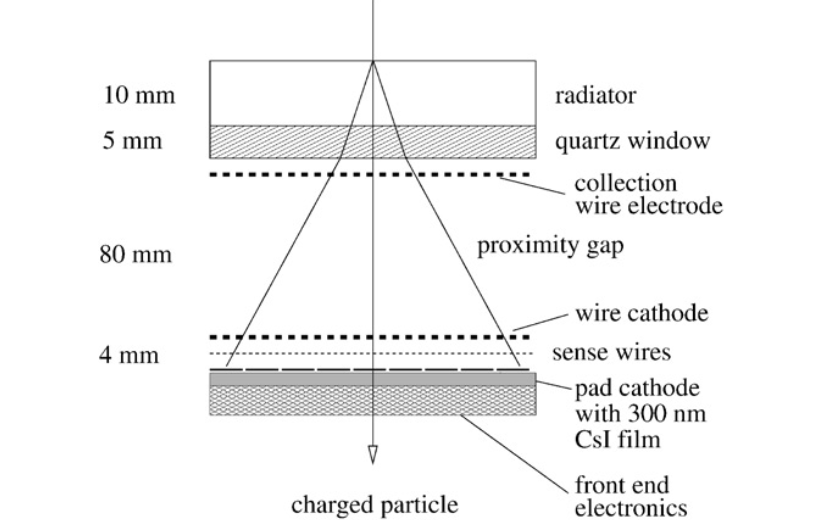
\includegraphics[scale=0.5]{STAR_Detectors/RICH_star_layout}
 		\caption{Δομή του Proximity Focusing RICH}
 		\label{fig3.21}
 	\end{figure}
 	
 	Στον RICH του STAR, ο Cherenkov Radiator είναι $C_6F_{14}$ σε υγρή μορφή και στην συνέχεια υπάρχει ένας κρύσταλλος χαλαζία. 
 	Χρησιμοποιείται η απλούστερη τεχνική Proximity Focusing για την κατεύθυνση των φωτονίων προς την ανιχνευτική περιοχή, κατά την οποία παρεμβάλλεται απλώς ένα στάδιο 80mm κενού χώρου μεταξύ του Radiator και των φωτοανιχνευτών. Ο σκοπός είναι να μεγαλώσει αρκετά η ακτίνα του κύκλου που εν τέλει θα προβληθεί στο επίπεδο του ανιχνευτή και έτσι να έχουε καλύτερη διακριτική ικανότητα.
 	
 	Στο ενδιάμεσο διάκενο ενδέχεται κάποια σωματίδια να ιονίσουν το υλικο και να προκύψουν ελεύθερα ηλεκτρόνια. Προκειμένου να τα απομακρύνουμε από την περιοχή ανίχνευσης έχουμε τοποθετήσει ανόδους κοντά στον Radiator για να τα συλλέγει.
 	Oι συλλογείς των ηλεκτρονίων από ιονισμό είναι τυπικοί Mulitiwire Proportional Chambers (MWPC), με αέριο μεθάνιο, του οποίου οι πρώτες κάθοδοι είναι 100μm σύρματα σε απόσταση 2.2mm από το επίπεδο των ανόδων οι οποίες είναι πάλι σύρματα 20μm που απέχουν μεταξύ τους 4.2mm. 
 	Στην τελική κάθοδο υπάρχουν τοποθετημένα 4 πανελ από ευαίσθητη περιοχή που δίνουν συνολική ενεργό περιοχή 1280$\times 800mm^2$. Στην επιφάνεια της τελικής καθόδου υπάρχει ο φωτομετατροπέας. Ένα λεπτό φιλμ από CsI όπου τα προσπίπτωντα φωτόνια Cherenkov αποβάλλουν ηλεκτρόνια μέσω φωτοηλεκτρικού φαινομένου τα οποία και εν τέλει ανιχνεύουμε ως ρεύμα. Μερικά αποτελέσματα του RICH φαίνονται στις επόμενες Εικόνες.
 	
 	\begin{figure}[h!]
 	    \centering
 	    \begin{minipage}{.5\textwidth}
 	        \centering
 	        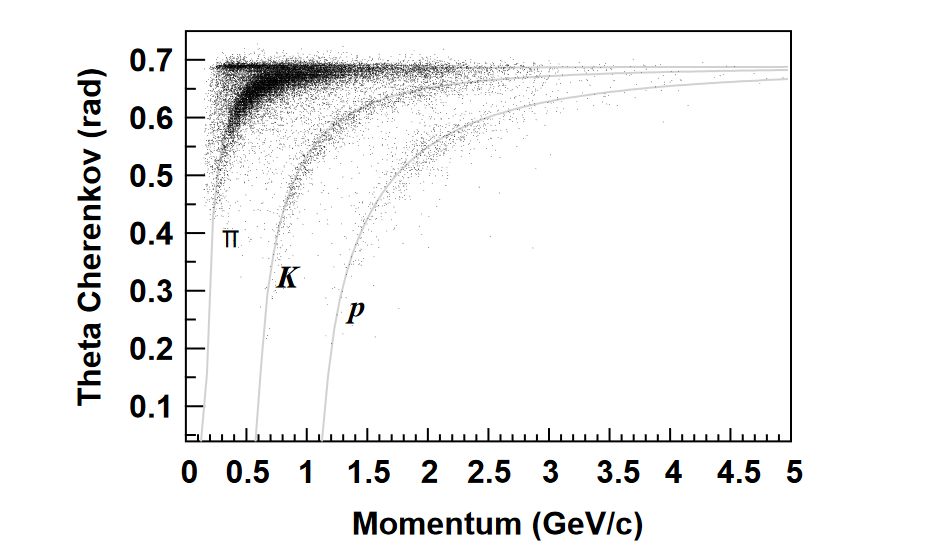
\includegraphics[scale=0.5]{STAR_Detectors/RICH_identif}
 	        \caption{Κατανομή της γωνίας Cherenkov συναρτήσει των μετρήσεων της ορμής που παρέχονται από τον TPC}
 	        \label{fig3.22}
 	    \end{minipage}%
 	    \begin{minipage}{0.5\textwidth}
 	        \centering
 	        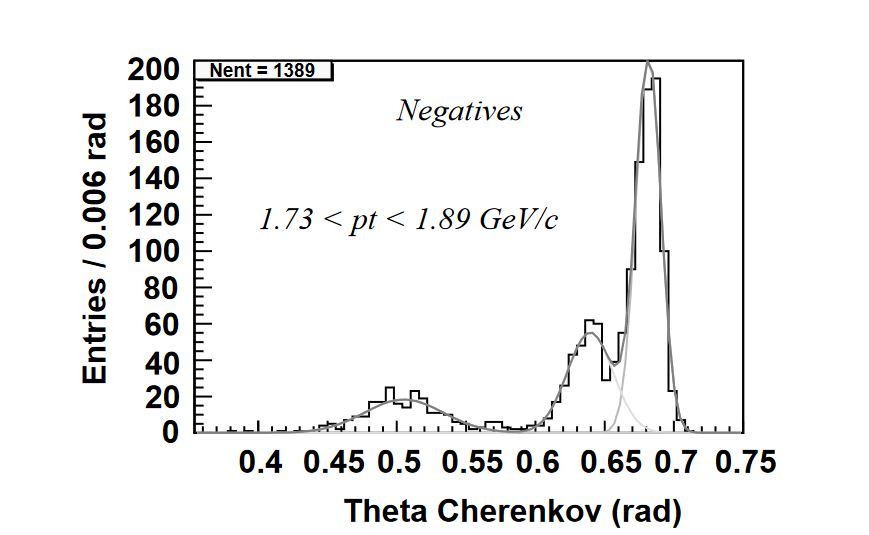
\includegraphics[scale=0.5]{STAR_Detectors/RICH_identif2}
 	        \caption{Ανιχνεύσεις σωματιδίων συναρτήσει της γωνίας Cherenkov για μικρό εύρος ορμών. Οι κορυφές αντιστοιχούν σε πιόνια, καόνια, πρωτόνια.}
 	        \label{fig3.22}
 	    \end{minipage}
 	\end{figure}
 	
 	
 	
\section{Photon Mulitplicity Detector (PMD)}

	Ο Photon Multiplicity Detector (PMD) του STAR, καλύπτει περιοχές pseudorapidity $2.3<\eta<2.5$, $\Delta \phi=2\pi$ και $p_t$ μικρή εως και 25MeV/c και θα μετράει την χωρική κατανομή των φωτονίων προκείμένου να μελετησει την ροή και τις διακυμάνσεις της.
	Χρησιμοποιείται έναντι των καλοριμέτρων σε περιοχές υψηλής πυκνότητας καθώς αν η περιοχή είναι πυκνή σε τροχιές, τότε οι καταιγισμοί των δευτερεύοντων σωματιδίων θα αλληλοεπικαλύπτονταν και ένα καλορίμετρο δεν θα μπορούσε να τις ξεχωρίσει. 
	Ας δούμε ποιοτικά την λειτουργία του PDM. 
	
	Η βασική δομή του PMD φαίνεται στην Εικόνα (\ref{fig3.24}).   
     Απαρτίζεται από διακριτά στοιχεία που είναι τοποθετημένα πίσω από ένα στρώμα μολύβδου. Τα φωτόνια που περνούν μέσα από το στρώμα του μολύβδου ξεκινούν έναν ηλεκτρομαγνητικό καταιγισμό και παράγουν ισχυρά σήματα. Αυτά τα σήματα δημιουργούνται στις κυψελίδες που υπάρχουν στα ευαίσθητα σημεία του ανιχνευτή. Η διαφορά με τα φορτισμένα αδρόνια είναι ότι εκείνα επηρεάζουν συνθήθως μόνο μία κυψελίδα, διότι δεν προκλούν καταιγισμό και έτσι παράγουν σήμα που αντιστοιχεί σε MIP. 
	To πάχος του μολυβδου είναι επιλεγμένο έτσι ώστε να παρέχει την βέλτιστη ισορροπία μεταξύ υψηλής πιθανότητας τα φωτόνια να κάνουν καταιγισμό και επίτευξη όσο το δυνατόν στενότερου πάχους για κάθε καταιγισμό ώστε να μειωθούν έχουμε αλληλοεπικαλύψεις καθώς θα υπάρχει περιβάλλον υψηλής πυκνότητας.
	Ακόμη, πριν από το κύριο τμήμα του ανιχνευτή, υπάρχει και ένα άλλο στρώμα, ο Veto Detector. Αυτός συνεισφέρει στο να εμποδίζει τα φορτισμένα σωματίδια απ΄ το να εισέρχονται στην περιχοή του μολύβδου όπου ξεκινάνε οι καταιγισμοί.
	\begin{figure}[h!]
		\centering
		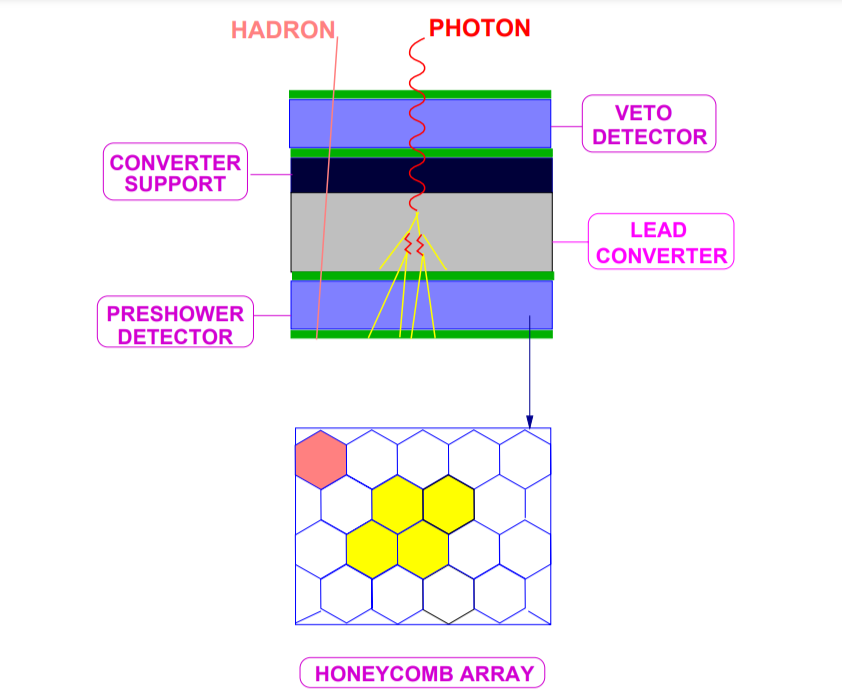
\includegraphics[scale=0.4]{STAR_Detectors/PMD_principle}
		\caption{Η βασική δομή και λειτουργία του PMD}
		\label{fig3.24}
	\end{figure}
	
	Τόσο ο Veto όσο και το ευαίσθητο τμήμα του PMD (Preshower Detector) αποτελούνται από εξαγωνικές κυψελίδες τοποθετημένες σε διάταξη κηρύθρας και η καθεμία είναι θάλαμος αερίων που λειτουργεί σε αναλογική περιοχή (ενδεικτικά στον Preshower υπάρχει μείγμα Ar/$CO_2$). 
	Ο σκελετός που αποτελεί τα όρια των κυψελίδων στην κηρύθρα είναι φτιαγμένος από χαλκό και ταυτόχρονα λειτουργεί ως κάθοδος αφού τον τοποθετούμε σε χαμηλό δυναμικό σε σχέση με το σύρμα ανόδου που υπάρχει στο κέντρο της κάθε κυψελίδας. 
	Μία συστοιχία από 24x24 κυψελίδες αποτελεί ένα \textit{module} και έχει ρομβικό σχήμα με πλευρά 254mm. Επίσης, κάποια modules από 4-9 είναι κλεισμένα εντός ενός αεροστεγούς θαλάμου ο οποίος αποτελεί το \textit{supermodule}. Συνολικά ο PMD αποτελείται από 24 supermodules. Στην Εικόνα (\ref{fig3.25}) φαίνεται η δομή μίας κυψελίδας καθώς και η συνολική εξαγωνική διάταξη των supermodules.
	
	\begin{figure}[h!]
		\centering
		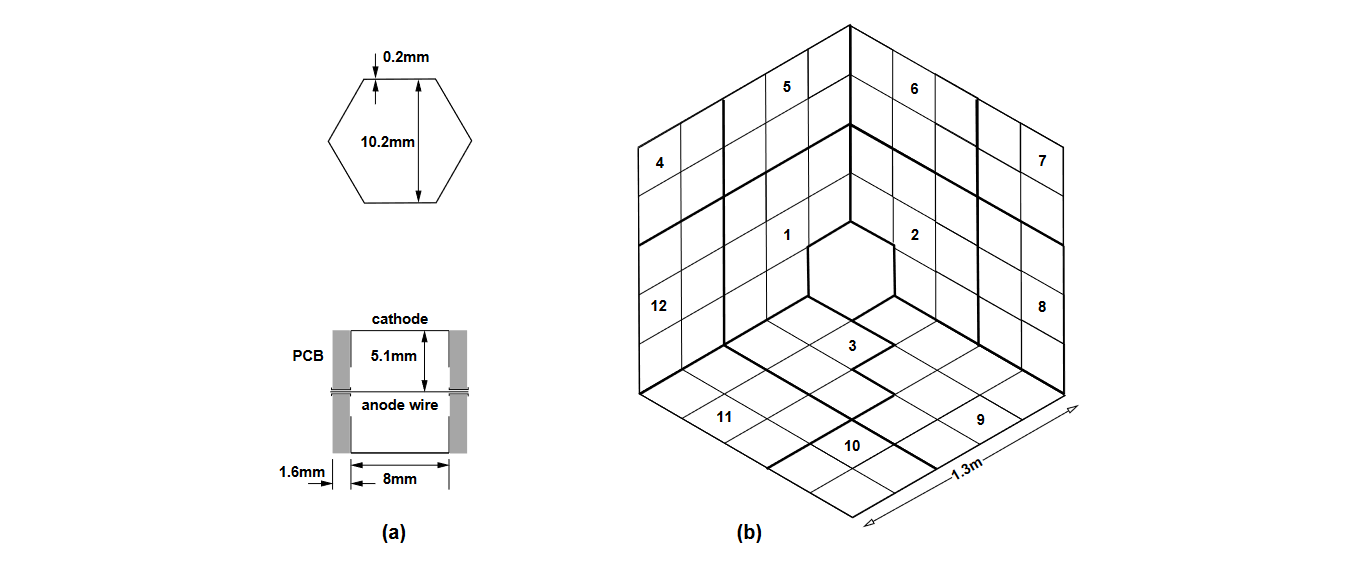
\includegraphics[scale=0.5]{STAR_Detectors/PMD_layout}
		\caption{(a) Δομή μίας κυψελίδας, (b) Διάταξη των modules σε supermodules η οποία καταλήγει σε ένα εξαγωνικό σχήμα.}
		\label{fig3.25}
	\end{figure}
	
	Όλες οι επιλογές των μερών που απαρτίζουν τον PMD έγιναν με γνώμονα τρεις στόχους, προκειμένου να είναι διαχειρήσιμη η υψηλή πυκνότητα εισερχόμενων σωματιδίων. Το σήμα των MIPs πρέπει να είναι περιορισμένο σε μία κυψελίδα, τα δ-ηλεκτρόνια με χαμηλή ενέργεια πρέπει να εμποδιστούν απ' το να ταξιδεύουν εως τις γειτονικές κυψελίδες προκαλώντας ανεπιθύμητη μεταφορά σήματος μεταξύ τους και τέλος η πιθανότητα ένα σωματίδιο να δώσει σήμα σε πολλές κυψελίδες να γίνει ελάχιστη.
%\section{Muon Telescope Detector {MTD}}
sfgsg
\section{Time of Flight Detector (TOF)}

	Το σύστημα Time of Flight (TOF), εγκαταστάθηκε στο STAR για την ταυτοποίηση των αδρονίων που παράγονται από τις συγκρούσεις βαρέων ιόντων. Αποτελείται από δύο υπο-ανιχνευτές, τον Pseudo Vertex Position Detector (pVPD) και τον Time of Fligh Patch (TOFp). 
	Ο πρώτος πρόκειται για τον ανιχνευτή που λαμβάνει το αρχικό σήμα, από την λήψη του οποίου ξεκινά η έναρξη του χρονομέτρου. Αποτελείται από δύο ξεχωριστά μέρη που τοποθετούνται δίπλα από τις βάσεις και έξω από τον μαγνήτη του STAR.
	Το κάθε μέρος απαρτίζεται από πλαστικούς σπινθηριστές των οποίων τα παραγόμενα φωτόνια οδηγούνται σε φωτοπολλαπλασιαστές.
	%Οταν ο TOFp λάβει σήμα, τότε σταματάει η καταμέτρηση του χρόνου. Αυτός βρίσκεται ακριβώς έξω από τον TPC
	
	Ο TOFp βρίσκεται ακριβώς έξω από τον TPC και όταν λάβει σήμα σταματάει η καταμέτρηση του χρόνου. Αποτελείται από 120 σειρές που τοπθετούνται γύρω από τον TPC. Η κάθε σειρά καλύπτει $6^o$ στην αζιμουθιακή διεύθυνση, έχει μήκος 2.4m και αποτελείται από 32 Multi-gap Resistive Plate Chambers (MRPC). 
	Ο MRPC  είναι μία συστοιχία από παράλληλα επίπεδα στο ενδιάμεσο των οποίων υπάρχει ένα αέριο.
	 Το κάθε επίπεδο αποτελεί ένα ηλεκτρόδιοστο οποίο εφαρμόζεται υψηλή τάση με αποτέλεσμα την δημιουργία ισχυρού πεδίου στο εσωτερικό τους. Όταν ένα φορτισμένο σωματίδιο διέρχεται από το αέριο δημιουργεί χιονοστοιβάδες Townsend και έτσι επάγεται φορτίο στα ηλεκτρόδια το οποίο ανινχεύεται ως σήμα.
	Η συνολική χρονική διακριτική ικανότητα του συστήματος είναι 100ps, κάτι που επιτρέπει ταυτοποίηση $\pi/K/p$ με ορμές έως και $1.6GeV/c$.
	
		\begin{figure}[h!]
				\centering
				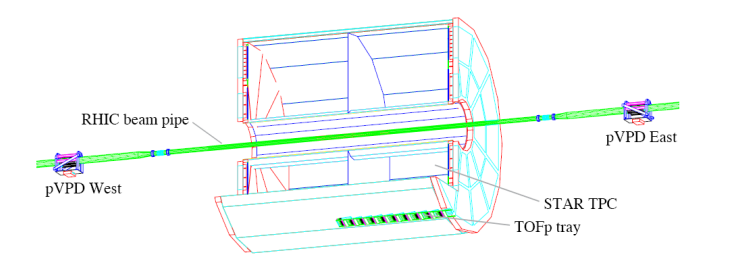
\includegraphics[scale=0.6]{STAR_Detectors/TOF}
				\caption{Οι θέσεις των υποανιχνευτών του συστήματος TOF}
				\label{fig3.27}
			\end{figure}
				
	
	Η ταυτοποίηση των σωματιδίων βασίζεται στον υπολογισμό της μάζας τους. Συγκεκριμένα, μετράται απ' ευθείας η ταχύτητα 
		\begin{align}\label{eq3.14}
			\frac{1}{\beta} = \frac{t-t_0}{\Delta s}c
		\end{align}
	όπου $\Delta s$ είναι το μήκος της τροχιάς του σωματιδίου όπως μετράται από τον TPC και $t_0$ είναι η στιγμή της κρούσης που μετράται από τον VPD. Έπειτα, η μάζα του σωματιδίου υπολογίζεται από την σχέση 
		\begin{align}\label{eq3.15}
			m = \frac{p}{c}\sqrt{\left(\frac{1}{\beta}\right)^2-1}
		\end{align}
	όπου η ορμή p μετράται από τον TPC.
\section{Zero Degree Calorimeter (ZDC) }

	Οι Zero Degree Calomieter (ZDC) ανιχνευτές αποτελούνται από τρια μέρη καλοριμέτρων. Το κάθε καλορίμετρο αποτελείται από διαδοχικά στρώματα βολφραμίου και ινών πλαστικού σπινθηριστή που παράγουν ένα οπτικό σήμα το οποίο ενισχύεται από έναν κοινό φωτοπολλαπλασιαστή, όπως φαίνεται στις Εικόνες (\ref{fig3.27}).
	
	\begin{figure}[h!]
		\centering
		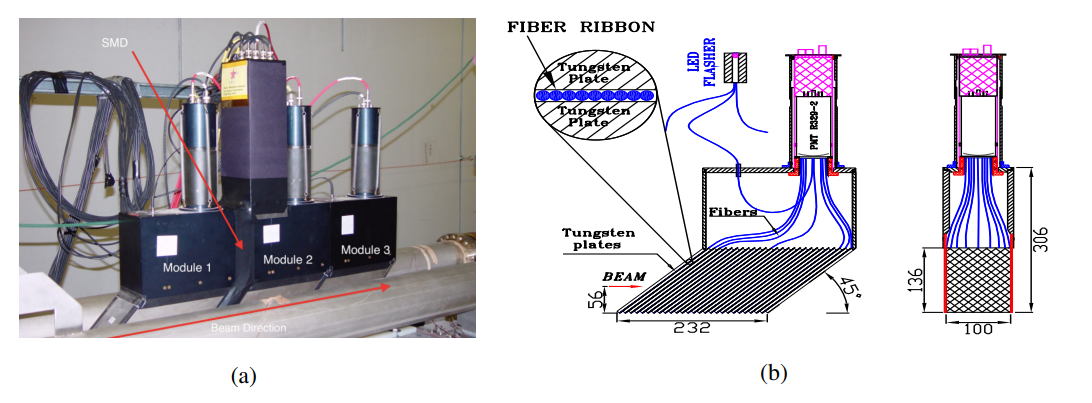
\includegraphics[scale=0.5]{STAR_Detectors/ZDC}
		\caption{Φωτογραφία του ZDC και σχέδιο του ενός από τα τρία μέρη του.}
		\label{fig3.27}
	\end{figure}
	
	Οι ZDC είναι σχεδιασμένοι για να ταυτοποιούν ουδέτερα σωματίδια και κυρίως νετρόνια που φέγουν από την περιοχή αλληλεπίδρασης σχεδόν παράλληλα με την δέσμη και ταυτόχονα παρέχουν πληροφορίες στο σύστημα \textit{trigger}. Είναι τοποθετημένοι και στις δύο πλευρές εκτός της περιοχής αλληλεπίδρασης 
\section{Data Acquisition System (DAQ) \& Triggers}

Ο ρόλος του Data Qcquuisition System (DAQ) είναι να διαβάσει τα δεδομένα που συλλέγονται από τους υποανιχνευτές του STAR και να τα μειώσε σε διαχειρήσιμα επίπεδα. Τα σημεία στα οποία λαμβάνονται οι αποφάσεις για το ποιά γεγονότα είναι κρίσιμα καλούνται \textit{triggers} και βασίζονται τόσο σε \textit{hardware}  όσο και σε \textit{software}. 
	Το \textit{trigger} γίνεται σε 4 επίπεδα. Τα πρώτα δύο 0 και 1 βασίζονται σε \textit{hardware} καθώς φιλτράρουν γεγονότα με μεγαλύτερη συχνότητα και πρέπει να αποκλείουν τα μη ενδιαφέροντα με μεγάλη ταχύτητα σε αντίθεση με τα 2 και 3 τα οποία βασίζονται σε \textit{software}.
	
	Κάποιες αποφάσεις στο επίπεδο 0 λαμβάνονται με βάση την ενέργεια που ενοποτίθεται σε ορισμένες περιοχές των BEMC \& EEMC. Έπειτα, τα δεδομένα των γεγονότων που περνάνε το πρώτο τεστ οδηγούνται στο επίπεδο 2 το οποίο πρόκειται για ένα πρόγραμμα που φιλτράρει μόνο τα γεγονότα ηλεκτρονίων ή φωτονίων. Αν κάποιο γεγονός περάσει και από το επίπεδο 2, τότε τα δεδομένα από όλα τα υποσυστήματα του STAR που σχετίζονται με αυτό το γεγονός θα οδηγηθούν στο σύστημα DAQ.
%\input{STAR_Systems/DAQ.tex}
%\input{STAR_Systems/Trigger.tex}
\chapter{Αποτελέσματα του STAR}

\section{Συγκρούσεις Βαρέων Ιόντων}

	Η QCD  είναι η θεμελιώδης θεωρία στην οποία βασίζεται η μελέτη των ισχυρών αλληλεπιδράσεων μεταξύ των Κουάρκ και των Γλουονίων και κατ΄επέκταση είναι αυτή που υπαγορεύει την δομή των αδρονίων και των πυρήνων.
	Η 	QCD επιβάλλει πως τα Κουάρκ και τα Γλουόνια είναι περιορισμένα εντός των αδρονίων τα οποία αποτελεούν την μόνη ευσταθή κατάσταση.
	
	Υπό ακραίες συνθήκες υψηλής θερμοκρασίας και πυκνότητας βαρυονίων, προβλέπεται πως συμβαίνει μία αλλαγή φάσης. Κατά αυτή την μετάβαση μπορούν να υπάρξουν ελεύθερα Κουάρκ και Γλουόνια και ονομάζεται, κατά το Ηλεκτρομαγνητικό ανάλογο, Πλάσμα Κουάρκ-Γλουονίων ( Quark-Gluon Plasma, GCP).  
	Αριθμητικές προβλέψεις υποδεικνύουν πως πράγματι συμβαίνει μία σχεδόν πρώτης τάξης αλλαγή φάσης σε μία κρίσιμη θερμοκρασία περίπου 170MeV(~2TeraKelvin).
	Αυτή η κατάσταση εικάζεται πως υπήρχει στα πρώτα κλάσματα του δευτερολέπτου μετά το Big Bang, πως επικρατεί στο εσωτερικό των αστέρων νετρονίων σε συνθήκες πολύ υψηλής πυκνότητας αλλά και πως μπορεί να δημιουργηθεί τεχνητά από συγκρούσεις βαρέων ιόντων.
		
	
	Πριν την κατασκευή του RHIC και των αντίστοιχων ανιχνευτών του, υπήρχαν ήδη άλλα πειράματα όπως το AGS και το SPS κατασκευασμένα την δεκαετία του 80' όπου ένας από τους στόχους τους χρησιμοποιώντας συγκρούσεις βαρέων ιόντων ήταν η εύρεση του QGP. 
	Όπως έχει αναφερθεί, μία από τις κύριες διεργασίες που συμβαίνουν στον RHIC είναι οι συγκρούσεις βαρέων ιόντων και κυρίως Au-Au με ενέργεια έως και $\sqrt{s}=200GeV/n$, δηλαδή συνολική ενέργεια περίπου 32TeV/ion .
	 Από την περίοδο κατασκευής του RHIC περίμεναν να δούν ενδείξεις για την δημιουργία του QGP καθώς η ανίχνευτή του αποτελούσε έναν από τους βασικούς στόχους του.
	Η εξέλιξη των συγκρούσεων βαρέων ιόντων φαίνεται στις Εικόνες (\ref{fig4.1})\&(\ref{fig4.2}). 
	
	\begin{figure}[h!]
	    \centering
	    \begin{minipage}{.5\textwidth}
	        \centering
	        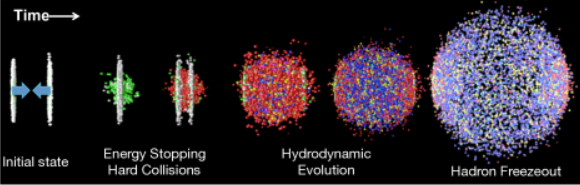
\includegraphics[scale=0.7]{STAR_Results/QGP_formation2}
	        \caption{Εξέλιξη των συγκρούσεων βαρέων ιόντων}
	        \label{fig4.1}
	    \end{minipage}%
	    \begin{minipage}{0.5\textwidth}
	        \centering
	        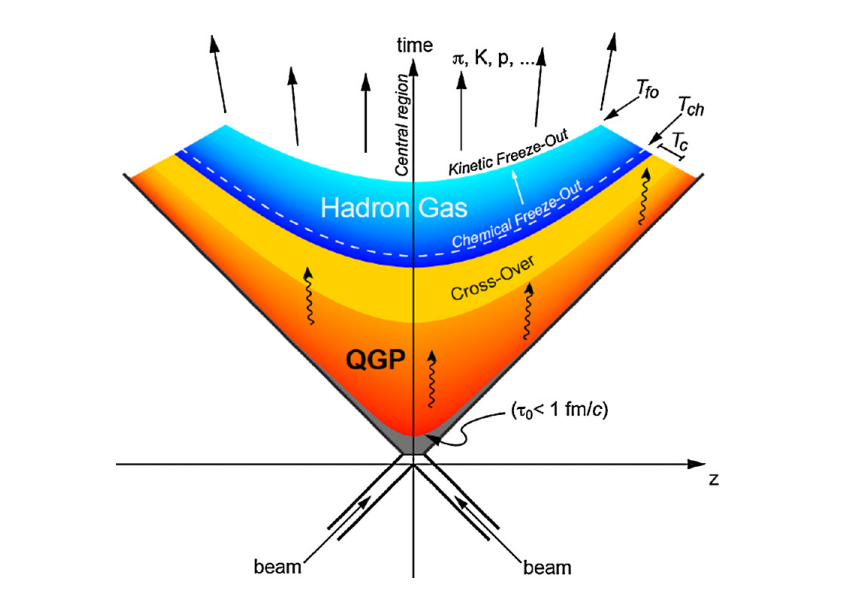
\includegraphics[scale=0.6]{STAR_Results/QGP_time_evolution}
	        \caption{Στάδια μετά την σύγκρουση βαρέων ιόντων}
	        \label{fig4.2}
	    \end{minipage}
	\end{figure}
	
	Πριν περάσουμε σε αποτελέσματα σχετικά με το πείραμα STAR που ένας στόχος του είναι η μελέτη κάποιων χαρακτηριστικών των παραπάνω συγκρούσεων θα πρέπει να δούμε 
πως ακριβώς αυτές εξελίσσονται και έπειτα να ορίσουμε το τί ακριβώς είναι το QGP. 		
	%Το  πρώτο στάδιο μετά την αλληλεπίδραση είναι αποδέσμευση των κουάρκ από τα αδρόνια και η δημιουργία του GQP, εάν βέβεια οι πυρήνες έχουν αρκετά μεγάλη ενέργεια.
	%Έπειτα, το σύστημα διστέλεται, πέφτει η θερμοκρασία του, έρχεται σε θερμική και χημική ισορροπία και ξανασχηματίζονται τα αδρόνια της τελικής κατάσταση τα οποία εν τέλει ανιχνεύουμε. Η χρονική κλίμακα που εξελίσσεται το φαίνόμενο είναι της τάξης $~10^{-23}$sec.
	Το αρχικό στάδιο, $\tau<0$\footnote{$\tau$ είναι ο proper time} είναι πριν την σύγκρουση	 όπου τα κουάρκ και τα γλουόνια υπάρχουν μέσα στα νετρόνια και τα πρωτόνιο με την συνάρτηση δομής τους.
	Μετά την σύγκρουση, για $0<\tau<\tau_0$, έρχεται το στάδιο των παρτονίων όπου η αρχική κινητική ενέργεια εναποτίθεται στην περιοχή επικάλυψης των πυρήνων. Αυτή η ενέργεια παράγει μία διεγερμένη κατάσταση της ύλης που καλείται \textit{fireball}. Αν αυτή η κινητική ενέργεια και η θερμοκρασία είναι αρκετά υψηλές, τότε δημιουργείται η κατάσταση στην οποία τα κουάρκ και τα γλουόνια αποδεσμεύονται από τα νουκλεόνια και φτιάχνουν το QGP.
	Στην συνέχεια, για $\tau_0<\tau<\tau_f$, οι συχνές αλληλεπιδράσεις και συγκρούσεις μεταξύ των συστατικών της \textit{fireball} οδηγούν το σύστημα σε θερμική ισοροπία και ταυτόχρονα λόγω της βαθμίδας της πίεσης σε διαστολή.
	Όσο το σύστημα διαστέλλεται ταυτόχρονα κρυώνει μέχρι να φτάσει σε μία κρίσιμη θερμοκρασία $T_c$, κάτω από την οποία αρχίζει η αδρονοποίηση, δηλαδή μία μετάβαση κατά την οποία τα αποδεσμευμένα κουάρκ και γλουόνια μετασχηματίζονται σε αδρόνια.
	%
	Τέλος, για $\tau>\tau_f$, είναι η φάση όπου επέρχεται χημική ισορροπία, δηλαδή καθώς το σύστημα συνεχίζει να διαστέλλεται, οι ανελαστικές συγκρούσεις παύουν (\textit{chemical freeze-out}) και στην συνέχεια καθώς η θερμοκρασία συνεχίζει να μειώνεται, η μέση ελεύθερη διαδρομή γίνεται μεγαλύτερη από το ίδιο το σύστημα και σταματούν ακόμη και οι ελστικές συγκρούσεις (\textit{kinetic freeze-out}). 
	Μετά από αυτό το σημείο τα αδρόνια κατευθύνονται προς τους ανιχνευτές μας.
	
	Όπως φαίνεται στην Εικόνα (\ref{fig4.1}) οι πυρήνες πριν την σύγκρουση είναι σχεδόν επίπεδοι, κάτι που προκύπτει άμεσα από την Ειδική Θεωρία της Σχετικότητας.
	% Αν θεωρήσουμε πως κινούνται κατά την κατεύθυνση z και έχουν ταχύτηα $\beta=99.999999$ της ταχύτητας του φωτός, 
	Δεδομένου ότι για ένα νουκλεόνιο στο σύστημα κέντρου μάζας έχουμε $\sqrt{s}=200GeV$, τότε για $Α=197$ νουκλεόνια θα έχουμε $E_{Au}=\sqrt{197\cdot s} = (197u) \gamma$. Tότε ο παράγοντας γ είναι  $\gamma=\left(1-\beta\right)^{-1/2}=15$. Από την βιβλιογραφία βρίσκουμε ότι η ακτίνα ενός ατόμου Χρυσού σε ένα σύστημα που το βλέπει ακίνητο είναι $r_0=166pm$. Άρα, από την συστολή του μήκους για σχετικιστικά κινούμενο παρατηρητή έχουμε ότι θα είναι περίπου 15 φορές μικρότερη $r'=r_0/\gamma\simeq 11pm$. Γι' αυτό και στην Εικόνα το άτομο Χρυσού φαίνεται σαν δίσκος.
	
	Για την θεωρητική μελέτη συγκρούσεων βαρέων ιόντων χρησιμοποιούνται διάφορα μοντέλα. Για παράδειγμα, η πιό απλή κατηγορία η οποία δεν δίνει την πλήρη δυναμική εξέλιξη του φαινομένου βασίζεται στην στατιστική φυσική. Εκεί το σύστημα περιγράφεται από μία Γενικευμένη Συνάρτηση Επιμερισμού (Grand Canonical Partition Function) και αποτελεί μία Μεγαλοκανονική συλλογή από μη αλληλεπιδρώντα φερμιόνια και μποζόνια σε θερμική και χημική ισοροπία. 
	Μία άλλη κατηγορία μοντέλων που παρέχουν μία απλή περιγραφή της δυναμικής εξέλιξης είναι τα υδροδυναμικά. Βασικές υποθέσεις εδώ είναι πως το σύστημα περιγράφεται από  νόμους διατήρησης (π.χ. εξίσωση συνέχειας) και από Καταστατικές Εξισώσεις (Equations of State) καθώς επίσης γίνεται υπόθεση για τοπική θερμική και χημική ισοροπία. Σε αυτό το μοντέλο οι αλληλεπιδράσεις δεν υπάρχουν από πρώτες αρχές αλλά είναι κρυμμένες στις ιδιότητες των ρευστών που περιγραφονται από κάποιες σταθερές μεταφοράς.
	Τέλος, τα πιό λεπτομερή μοντέλα είναι αυτά που πρεριγράφουν μικροσκοπικά τις ιδιότητες μεταφοράς (Microscopic Transport Models). Αυτά βασίζονται στην θεωρία μεταφοράς για σχετικικστή κβαντομηχανική πολλών σωμάτων και λαμβάνουν υπ' οψιν τις αλληλεπιδράσεις όλων των βαθμών ελευθερίας μέσω δυναμικών και ενεργών διατομών.
	
	Όπως και στο ΗΜ πλάσμα η κοινότυπη πρόταση που ακούει κανείς ότι "πλάσμα είναι ένα ιονισμένο αέριο" είναι λάθος, ή τουλάχιστον δεν είναι πλήρως σωστή, έτσι και στο QGP το να πούμε ότι απλώς είναι η κατάσταση στην οποία τα κουάρκ και τα γλουόνια δεν σχηματίζουν αδρονικές καταστάσεις είναι εν μέρει απλούστευση. 
	Εδώ θα χρησιμοποιηθεί ο ορισμός της αναφοράς \cite{dd}
	\begin{quote}
		\textit{Πλάσμα Κουάρκ Γλουονίων είναι μία κατάσταση της ύλης που βρίσκεται σε τοπική θερμική ισορροπία και στην οποία τα κουαρκ και τα γλουόνια δεν συγκρατούνται εντός των αδρονίων έτσι ώστε οι βαθμοί ελευθερίας του χρώματος να γίνονται αντιληπτοί σε όλον τον όγκο}
	\end{quote}
	
	Η θερμοποίηση (thermalization), δηλαδή η επίτευξη της θερμικής ισορροπίας μέσω 
αλληλεπιδράσεων των συστατικών του συστήματος, θεωρείται αναγκαία συνθήκη για την μελέτη αυτής της κατάστασης η οποία να μπορεί να συγκριθεί με τις προβλέψεις της QCD αλλά και να θεωρηθεί πως υπήρχε στα πρώτα κλάσματα μετά το Big Bang. 
	Οι πυρηνικές σκεδάσεις παράγουν μεγάλη αριθμητική πυκνότητα σωματιδίων και ενέργειας και για να μπορέσουμε να μιλήσουμε για μία κατάσταση της ύλης σε τοπική θερμοδυναμική ισορροπία που χαρακτηρίζεται από παραμέτρους όπως η θερμοκρασία, η πίεση, η πυκνότητα ενέργειας, θα πρέπει να έχει επέλθει η θερμοποίηση του συστήματος.
	Δεν υπάρχει κάποια \textit{απαίτηση} για ενδείξεις μετάβασης φάσης πρώτης ή δεύτερης τάξης, παρόλο που υπάρχουν ενδείξεις για απότομες αλλαγές σε παρατηρήσιμα μεγέθη.
	
	\subsection{Αδρή περιγραφή των μοντέλων για την μελέτη του QGP}
	
	Το διάγραμμα φάσης (Εικόνα (\ref{fig4.3})) θα πρέπει να περιγράφεται από την QCD. Όπως αναμένουμε θα πρέπει επίσης σε υψηλές θερμοκρασίες να αποδεσμεύονται τα κουάρκ και τα γλουόνια περέχοντας έτσι νέους βαθμούς ελευθερίας χρώματος και αυξάνεται η εντροπία άρα και η πίεση με την αύξηση της θερμοκρασίας. 
	Κάνοντας κάποιες εμφανώς λανθασμένες παραδοχές, δηλαδή πως τα κουάρκ και τα γλουόνια δεν αλλληλπιδρούν και πως επίσης τα κουάρκ έχουν μηδενική μάζα, μπορούμε να βρούμε ότι η πίεση αυτής της κατάσταση συναρτήσει της θερμοκρασίας και για μηδενικό χημικό δυνναμικό βαρυονικού αριθμού, καθορίζεται από τους βαθμούς ελευθερίας από έναν νόμο τύπου Stefan-Boltzman 
	\begin{align*}\label{eq4.1}
		\frac{P_{SB}}{T^4 }= \left[ 2(N_c^2-1)+\frac{7}{2}N_cN_f\right] \frac{\pi^2}{90} \numberthis
	\end{align*}
	
	
	\begin{figure}[h!]
		\centering
		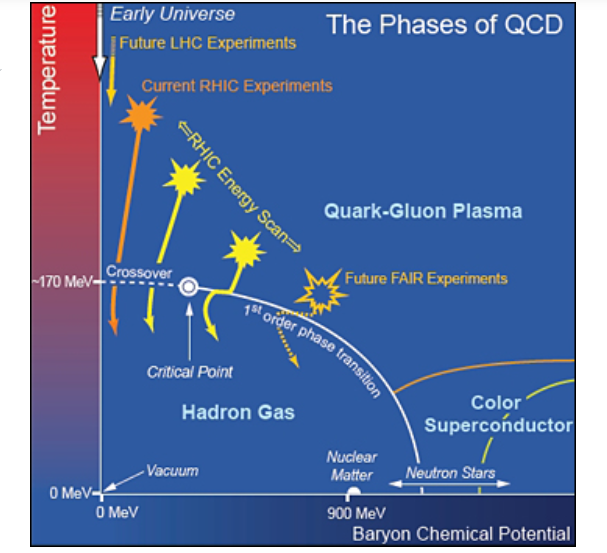
\includegraphics[scale=0.7]{STAR_results/QCD_phase_diagram}
		\caption{Διάγραμμα Φάσης Θερμοκρασίας, Θερμοκρασία συναρτήσει του χημικού δυναμικού των βαρυονίων. Η χρήση της πυκνότητας του χημικού δυναμικού για τον βαρυονικό αριθμό θα έδινε αντίστοιχο διάγραμμα φάσεων. Αυτό μπορούμε να το δούμε διαισθητικά αν θεωρήσουμε το σύστημα ως ένα αέριο φερμιονίων. Εκεί έχουμε ότι $\mu\sim E_f \sim p_F^2 \sim   density^{2/3}$}
		\label{fig4.3}
	\end{figure}
	
	
	Αριθμητικοί υπολογισμοί στην LQCD(Lattice QCD) έχουν δώσει αποτελέσματα τα οποία δίνουν αλλαγή φάσης για μηδενικό βαρυονικό χημικό δυναμικό σε θερμοκρασία περίπου 170MeV. Για παράδειγμα στην Εικόνα (\ref{fig4.4}) φαίνεται πως περίπου σε αυτή την θερμοκρασία υπάρχει έντονη μεταβολή του μεγέθους $P/T^4$ το οποίο έρχεται σε κορεσμό περίπου στην διπλάσια θερμοκρασία για διάφορες παραδοχές για τις γεύσεις των κουάρκ. Φαίνεται επίσης η σύγκριση των εν λόγω υπολογισμών με τα αποτελέσματα της σχεσης (\ref{eq4.1}). Αυτή η διαφορά υποδεικνύει πως οι αλληλεπιδράσεις και η μάζα των κουάρκ έχουν σημαντικό ρόλο στην μελέτη, όπως είναι και το προφανές.
	
	
	\begin{figure}[h!]
		\centering
		\includegraphics[scale=0.7]{STAR_Results/Predictions/P_over_T4_diagaram}
		\caption{Διάγραμμα πίεσης ανά $T^4$ συναρτήσει της θερμοκρασίας που έχει προκύψει από υπολογισμούς στην LWQCD και στο οποίο φαίνεται η πιθανή αλλαγή φάση  σε θερμοκρασία ~170MeV}
		\label{fig4.4}
	\end{figure}
	
	%Υπάρχουν επίσης υδροδυναμικά μοντέλα τα οποία στοχεύουν στο να υπολογίσουν την κάθετη ροή των προϊόντνω της σκέδασης. Αυτά προβλέπουν πως αυτή η ροή θα έχει ελλειπτικό σχήμα και λειτουργούν επίσης σε καταστάσεις ισορροπίας μέσω καταστατικών εξισώσεων.
	%Ακόμη, τα στατιστικά μοντέλα περιγράφουν την μακροσκοπική συμπεριφορά της κατάστασης ισοροπίας, αλλά δεν περιγράφουν τον τρόπο με τον οποία επιτυγχάνεται.
\subsection{Μερικά από τα αποτελέσματα των πρώτων χρόνων λειτουργίας του STAR}	
	
	Οι μετρήσεις των τελικών αδρονίων από τις συγκρούσεις βαρέων ιόντων αποκάλυψαν πως υπάρχουν τρεις διακριτές περιοχές της κάθετης στην δέσμη ορμής όπου έχουμε διαφορετική συμποεριφορά. Η "\textit{soft range}" $p_T\leq 1.5GeV/c$ η οποία περιέχει και το μεγαλύτερο πλήθος αδρονίων, η "\textit{hard-scattering range}" με $p_T\geq 6GeV/c$ η οποία παρέχει αποτελέσματα για τις καταστάσεις των παρτονίων στα πρώτα στάδια των κρούσεων. Ακόμη υπάρχει και η ενδιάμεση περιοχή "\textit{intermediate range}", με $1.5\leq p_T\leq 6GeV/c$ όπου περιέχονται ταυτόχρονα διαδικασίες και καταστάσεις και από τις προηγούμενες δύο περοχές. 	
	
	Αρχικά στην \textit{soft} περιοχή έχει παρατηρηθεί πως η ύλη που παράγεται παρουσιάζει συλλογική ροή\footnote{Η ροή εδώ αναφέρεται στην εξάρτηση της ενέργειας, της ορμής και της αριθμητικής πυκνότητας των σωματιδίων από την κατεύθυνση.}. 
	Γενικά, υπάρχει ένα μέτρο της μη ισοτροπικής ροής προς όλες της κατευθύνσεις το οποίο λέγεται \textit{elliptic flow}. Συγκεκριμένα περιγράφει την ανισοτροπικότητα της ροής στην αζιμουθιακή διεύθυνση $\phi$ σε ένα επίπεδο κάθετο στην δέσμη. 
	%Ορίζεται ως ο δεύτερος συντελεστής Fourier, από το ανάπτυγμα σε τριγωνομετρική σειρά Fourier της συνάρτησης $d^3N/d^3\bm{p}$, όπου $\bm{p}$ η ορμή ενός σωματιδίου, και Ν ο αριθμός των αλληλεπιδρώντων σωματιδίων και προκύπτει ότι είναι 
%	\begin{align*}\label{eq4.2}	
%		u_2 (p_t,y)=\braket{cos(2[(\phi-\Psi_{RP}])} \numberthis
%	\end{align*}
%	όπου $\phi$ είναι η αζιμουθιακή γωνία και $\Psi_{RP}$ είναι η γωνία του  επιπέδου που σχηματίζει το διάνυσμα της κατεύθυνσης της δέσμης με το διάνυσμα παραμέτρου κρούσης που ενώνει τα κέντρα των δύο ιόντων με  τον άξονα.
	
	Όταν τα τα προϊόντα της κρούσης έρθουν σε χαμηλότερη θερμοκρασία, τότε η ορμή των σωματιδίων μεταφέρεται στα τελικά αδρόνια που σχηματίζονται. Αυτά είναι που ανιχνεύουμε και ο ροή των οποίων μπορεί να μας οδηγήσει σε συμπεράσματα για την πρώτερη κατάσταση και η ανισοτροπικότητά της αποτελεί ένδειξη για την δημιουργία του QGP.
	Η αζιμουθιακή κατανομή των σωματιδίων είναι περιοδική συνάρτηση του $\phi$ και γράφεται ως σειρά Fourier. 
	\begin{align*}\label{eq4.2}
		f(\phi) = \frac{\alpha_0}{2\pi} + \frac{1}{\pi} \left( \sum_{n=1}^\infty \alpha_n cos(n\phi) + b_n sin(n\phi)\right) \numberthis
	\end{align*}
	%
	Όπου $\alpha_n$, $b_n$ οι συνηθισμένοι συντελεστές Fourier με $\alpha_0=N$. Αν θέσουμε $-\pi/n < \psi_n < \pi/n$ και $\omega_n =\sqrt{\alpha_n^2+b_n^2}$ τότε γίνεται 
	\begin{align*}\label{eq4.3}
		f(\phi) = \frac{N}{2\pi}\left( 1 + \sum_{n=1}^\infty 2\underbrace{\frac{\omega_n}{\omega_0}}_{v_n}cos(n(\phi-\psi_n) )\right) \numberthis
	\end{align*}
 Όπου οι συντελεστές ροής $v_n$ που σχετίζονται με το σχήμα και την ανισοτροπικότητα της ροής δίνονται από την σχέση 
 	\begin{align*}\label{eq4.4}
 		v_n = \braket{ cos(n(\phi-\psi_n))} \numberthis
 	\end{align*}
 	
 	Ενδεικτικά ο συντελεστής $v_2$ ονομάζεται \textit{elliptical flow} και αναπαριστά την εκκεντρότητα της ελλειψοειδώς ανισοτροπικής ροής που προκύπτει από μία \textit{peripheral} συγκρουση.
 
	Τα τελικά αδρόνια στην \textit{soft} περιοχή φαίνεται να ακολουθούν μία κίνηση υπό ένα κοινό, κάθετο στην δέσμη, πεδίο ταχυτήτων που επηρεάζεται από τις συνθήκες που επικρατούσαν στην αρχή της σκέδασης όπου είχαμε γρήγορη διαστολή των προϊόντνω υπό ένα μη ισοτροπικό πεδίο πίεσης και συχνές αλληλεπιδράσεις.
	Η συλλογικότητα της ροής φαίνεται από την εξάρτηση του συντελεστή \textit{elliptic flow} από την μάζα των τελικών αδρονίων σε χαμηλή $p_T$, Εικόνα (\ref{fig4.5}). Τα πειραματικά δεδομένα φαίνεται να συμπίπτουν με τους υδροδυναμικούς υπολογισμούς που υποθέτουν σύντομη θερμοποίηση, εκτόνωση σαν ιδανικό αέριο, αλλαγή φάσης σε θερμοκρασία περίπου 170MeV. 

\begin{figure}[h!]
	\centering
	\includegraphics[scale=0.8]{STAR_Results/result_soft_1}
	\caption{Εξάρτηση του συντελεστή $v_2$ από την ορμή $p_T$ σε συγκρούσεις 200GeV/n Au-Au. Φαίνεται έτσι η συλλογική ροή των παραγόμενων σωματιδίων. }
	\label{fig4.5}
\end{figure}

	Ένα άλλο αποτέλεσμα είναι ότι οι περισσότερες ιδιότητες του κύριου όγκου που μετρήθηκαν φαίνονται παρόμοιες με αυτές που προέκυπταν από συγκρούσεις βαρέων ιόντων σε χαμηλότερες ενέργειες (ενδεικτικά αποτελέσματα στις Εικόνες (\ref{fig4.6}) \& (\ref{fig4.7})).
	 Πριν από τα αποτλέσματα του STAR οι θεωρητικές προβλέψεις πρότειναν ισχυρή εξάρτηση των εν  λόγωιδιοτήτων από την ενέργεια.
	Η παρατηρούμενη ομαλή συμπεριφορά των ιδιοτήτων αρχικά αποδόθηκε στο ότι το QGP  δημιουργείται από ένα εύρος αρχικών τοπικών συνθηκών, ακόμη και για δεδομένη ενέργεια και παράμετρο κρούσης.
	Στην Εικόνα (\ref{fig4.6}) παρατηρούμε πως η εξάρτηση του συντελεστή $v_2$ \textit{elliptical flow} από την ενέργεια, στην \textit{soft} περιοχή των συγκρούσεων υψηλής ενέργειας, είναι κοντά με την εξάρτηση του αντίστοιχου συντελεστή των συγκρούσεων χαμηλότερης ενέργειας.
	Στην Εικόνα (\ref{fig4.7}) φαίνεται η συνδιασπορά στην ορμή $p_T$ φορτισμένων σωματιδίων συναρτήσει του αριθμού των σωματιδίων $N_{part}$ που λαμβάνουν μέρος στην κρούση από την οποίο εξαρτάται η κεντρικότητα.
	%
	Η κεντρικότητα (centrality) ορίζεται ως το ποσοστό της ενεργού διατομής από ένα κατώφλι σωματδίων ως προς την συνολική ενεργό διατομή  
	\begin{align*}\label{eq4.5}
			%c(b) = \frac{\pi b^2}{\sigma_{inel}}  
			c = \frac{1}{\sigma_{AA}}\int_{N_{ch}^{thresh}}^{\infty} \odv{\sigma}{N_ch}'dN_{ch}' \propto \frac{1}{N_{part}}\numberthis
		\end{align*}	
	όπου b η παράμετρος κρούσης, δηλαδή η απόσταση των κέντρων των δύο πυρήνων και $\sigma_{inel}$ η συνολική ενεργός διατομή της σκέδασης. Πρόκεται για ένα μέτρο του πόσο κεντρική είναι η κρούση.
	
	
	\begin{figure}[h!]
	    \centering
	    \begin{minipage}{.5\textwidth}
	        \centering
	        \includegraphics[scale=0.7]{STAR_Results/energy_dependence_of_v2}
	        \caption{Εξάρτηση του συντελεστή \textit{ellipitic flow} από την ενέργεια}
	        \label{fig4.6}
	    \end{minipage}%
	    \begin{minipage}{0.5\textwidth}
	        \centering
	        \includegraphics[scale=0.7]{STAR_Results/momentum_covariance_4_charged_particle_pairs}
	        \caption{Εξάρτηση της ρίζας της συνδιασποράς για ζεύγη φορτισμένων σωματιδίων  (προς την $p_T$) από την κεντρικότητα για διάφορες τιμές ενεργειών}
	        \label{fig4.7}
	    \end{minipage}
	\end{figure}
	
	
%	Ένα τελευταίο αποτέλεσμα σχετικό με την \textit{soft} περιοχή είναι η παραγωγή διαφορετικών ειδών, έως και strange, βαρυονίων γίνεται συνεπής με την Μεγαλοκανονική Κατανομή σε με
%	
%\begin{figure}[h!]
%	\centering
%	\includegraphics[scale=0.7]{STAR_Results/results_good_statistical1}
%	\caption{Προβλέψεις της στατιστικής θεωρίας για την λόγο διάφορων αδρονίων (μπλέ γραμμές) σε σύγκριση με τα περιαμταικά αποτελέσματα σε συγκρούσεις 200GeV}
%	\label{fig4.8}
%\end{figure}

	Σχετικά με την  \textit{intermediate} $p_T$ περιοχή.
Εδώ επέρχεται κορεσμός του \textit{elliptic flow, $v_2$}, δηλαδή η ροή τείνει προς την ισοτροπική (Εικονα (\ref{fig4.8})) και βλέπουμε διαφορές στην πυκνότητα και την $v_2$ βαρυονίων-μεσονίων. 
	Για παράδειγμα στην Εικόνα (\ref{fig4.9}) βλέπουμε το $R_{CP}$ συναρτήσει της $p_T$. Το $R_{CP}$ σχετίζεται με τον λόγο των κεντρικών συγκρούσεων (b=0) προς των peripheral συγκρούσεων ($0<b<R_1+R_2$). Εκεί βλέπουμε ότι ο λόγος $R_{CP}$ δεν σχετίζεται με την μάζα των βαρυονίων/μεσονίων αλλά σχετίζεται με τον άν πρόκειται για βαρυόνιο η μεσόνιο. 
	

		
		\begin{figure}[h!]
		    \centering
		    \begin{minipage}{.5\textwidth}
		        \centering
		        \includegraphics[width=1.1\linewidth, height=0.2\textheight]{STAR_Results/results_intermediate}
		        \caption{Κορεσμός του \textit{elliptical flow} στην intermediate περιοχή}
		        \label{fig4.8}
		    \end{minipage}%
		    \begin{minipage}{0.5\textwidth}
		        \centering
		        \includegraphics[width=1.1\linewidth, height=0.2\textheight]{STAR_Results/results_intermediate2}
		        \caption{Λόγος κεντρικών προς peripheral συγκρούσεων για μεσόνια και βαρυόνια συναρτήσει της $p_T$}
		        \label{fig4.9}
		    \end{minipage}
		\end{figure}   
	
	Ακόμη, υπήρχε άλλη μία ένδειξη πως στην δημιουργία του QGP ευνοοείται ο σχηματισμός \textit{strange} αδρνίων, δηλαδή αδρονίων που περιλαμβάνουν ένα τουλάχιστον \textit{strange } κουάρκ. Στις συνήθεις αδρονικές αντιδράσεις η παραγωγή των \textit{strange} κουάρκ καταπιέζεται εξαιτίας της μεγάλης τους μάζας ($m_s\simeq 95MeV/c^2$ ) σε σύγκριση με τα \textit{up} και \textit{down} ($m_u\simeq2.2MeV/c^2, m_d\simeq4.7MeV/c^2$). 
	Όμως στην φάση που δημιουργείται το QGP η θερμοκρασία που επικρατεί ευνοεί την παραγωγή \textit{strange} κουάρκ  και κατ' επέκταση ζεύγων $s\bar{s}$. Αυτό γίνεται αντιληπτό από την παραγωγή βαρυονίων και μεσονίων που περιέχουν $s$ ή $\bar{s}$. 
	Δεδομένου οτι τα Καόνια αποτελούνται από ένα \textit{strange} αντικουάρκ ($K^+(u\bar{s}), K^0(d\bar{s})$) και τα Πιόνια μόνο από \textit{up \& down} κουάρκ    ($\pi^+(u\bar{d}), \pi^0(u\bar{u},d\bar{d})$), αν μετρήσουμε τον λόγο παραγωγής τους, τότε θα δούμε ότι υπάρχει όντως μία αυξημένη παρουσία των Καονίων στην φάση του QGP στην περιοχή μέσης rapidity, άρα και μέσης ορμής. Αυτά τα αποτελέσματα του STAR φαίνονται στην Εικόνα (\ref{fig4.10}) όπου η παραγωγή s κουάρκ ευνοείται στις συγκρούσεις Au-Au έναντι των p-p.
	
	\begin{figure}[h!]
		\centering
		\includegraphics[scale=0.7]{STAR_Results/strange_enhancement}
		\caption{Λόγος της παραγωγής Κ/$\pi$ συναρτήσει της ορμής}
		\label{fig4.10}
	\end{figure}
	
%%%%%%%%%%%%%%%%%%%%%%%  HARD SECTOR	%%%%%%%%%%%%%%%%%%%%%%
		Τέλος, σχετικά με την \textit{hard} περιοχή. 
	%Το κύριο χαρακτηριστικό εκεί είναι ο κορεσμός σε υψηλό επίπεδο της \textcolor{red}{κατάπνιξης} (\textiit{suppression}) των αδρονίων , συγκριτικά με τις αναμενόμενες από άλλες συγκρούσεις p-p, peripheral Au-Au. \textit{Suppression} αδρονίων είναι όταν τα αδρόνια παράγονται σε χαμηλό ποσοστό από τα 
	Το κύριο χαρακτηριστικό είναι η ισχυρή καταπίεση (suppression) της παραγωγής αδρονίων και μεσονίων όπως το J/$\psi$ σε κεντρικές  συγκρούσεις Au-Au, το οποίο θεωρείται ως ένδειξη για την δημιουργία του QGP. Καθώς τα κουάρκ και τα αντικουάρκ αποδεσμεύονται από τα αδρόνια και τα μεσόνια δημιουργείται χωρικό φορτίο χρώματος και κατ'επέκταση μία θωράκιση της ισχυρής πυρηνικής δύναμης κάπως ανάλογα με την θωράκιση Debye στα αέρια ελεύθερων ηλεκτρονίων. Τότε, αυτή η θωράκιση εμποδίζει την δημιουργία καταστάσεων με πολλά κουάρκ καθώς μειώνεται η μεταξύ τους αλληλεπίδραση.
	%Experimenta and theoretical... pg 167 2nd bullet
	
\begin{figure}[h!]
	\centering
	\includegraphics[scale=0]{STAR_Results/strange_enhancement}
	\textcolor{white}{\caption{Μέιωση της παραγωγής αδρονίων όσο αυξάνεται η ορμή $p_T$}}
	\label{fig4.11}
\end{figure}

	Μία ακόμη ένδειξη για την δημιουργία του QGP που προέρχεται από την περιοχή υψηλών ορμών είναι η το φαινόμενο \textit{jet quenching}. 
	Οι ισχυρές συγκρούσεις παρτονίων οδηγούν σε παραγωγή κουάρκ και γλουονίων με μεγάλη ορμή τα οποία διαχωρίζονται σε έναν μεγάλο αριθμό από ισχρά κατευθυνόμενα αδρονια, τα jets. 
	Τα jets, δημιουργούνται σε αρχικά στάδια της σύγκρουσης των βαρέων ιόντων πολύ πριν την δημιουργία της πυκνής ύλης. Τα jet θα "αισθανθούν" την πλήρη εξέλιξη της σύγκρουσης και έτσι θα φέρουν πληροφορίες και από την φάση όπου δημιουργείται η πυκνή και θερμή ύλη. Επειδή η πλειοψηφία των ισχυρών συγκρούσεων είναι μεταξύ δύο σωμάτων, θα παρατηρούμε δύο jets. Σε συγκρούσεις Au-Au,  υπάρχει η πιθανότητα τα jets να γεννηθούν κοντά στην δημιουργία του QGP. Τότε το ένα απ' τα δύο jets κάποιου γεγονότος θα εκπεμφθεί προς την μία μερία, απομακρυνόμενο από το QGP, ενώ το άλλο θα περάσει αναγκστικά από το εσωτερικό του QGP.
	Τώρα, αν όντως το QGP υπάρχει, τότε τα παρτόνια του jet που περνάει από το εσωτερικό του μπορεί να χάσουν τόση ενέργεια ώστε να μην προλάβουν να δημιουργηθούν αδρόνια. Αυτό το φαινόμενο είναι το \textit{jet quenching}.
	
	Για να μετρηθεί το \textit{jet quenching} σε πειράματα βαρέων ιόντων, πρέπει να χρησιμοποιηθεί η συσχέτιση (correlation) ανάμεσα σε δύο αδρόνια υψηλής ορμής.
	Αν μετρηθεί ένα τέτοιο αδρόνιο, που υποθέτουμε ότι προέρχεται από jet, τότε θα πρέπει να μετρηθεί και άλλο ένα με διαφορά αζιμουθιακης γωνίας $\Delta\phi=\pi$. Αν δεν μετρηθεί τότε θεωρούμε πως το δεύτερο jet έχει διέλθει εντός του QGP και έχει καταπνιχθεί. 
	Αυτό φαίνεται στην Εικόνα (\ref{fig4.12}) όπου σε συγκρούσεις d-Au \& p-p  παρατηρείται και δεύτερο jet, ενώ σε συγκρούσεις Au-Au δεν παρατηρείται και έτσι θεωρούμε πως εκεί δημιουργείται QGP.
	
	\begin{figure}[h!]
		\centering
		\includegraphics[scale=0.9]{STAR_Results/jet_quenching}
		\caption{Το δεύτερο jet αδρονίου δεν παρατηρείται σε γωνία π από το πρώτο}
		\label{fig4.12}
	\end{figure}
	
	
	\subsection{Γενικότερα Αποτελέσματα}	
		\subsubsection{Πρώτη Παρατήρηση του (anti-)Hypertriton }
						
		Ένα μικρό, αλλά σημαντικό, ποσοστό των παραγόμενων σωματιδίων μία σύγκρουσης βαρέων ιόντων αποτελούν και οι ελαφρείς πυρήνες. Παρατηρήθηκαν $70\pm17$ anti-hypertriton και $157\pm30$ hypertriton πυρήνες, με τους πρώτους να παρατηρθούνται για πρώτη φορά στο STAR έπειτα από συγκρούσεις Au-Au. Ο anti-hypertriton  πυρήνας αποτελείται από αντιπρωτόνιο, αντινετρόνιο και ένα αντι-Λαμδα ($\Lambda$). Η μελέτη των χαρακτηριστικών του παραπάνω ζεύγους πυρήνα-αντιπυρήνα μπορεί να οδηγήσει σε έλεγχο της συμμετρίας CPT για την οποία μέχρι στιγμής δεν έχει βρεθεί κάποια παραβίαση. 
			
			Επειδή ο εν λόγω πυρήνας είναι πολύ ασταθής δεν μπορεί να ανιχνευθεί ευθέως και γι'αυτό ανιχνεύουμε τα προίόντα των διασπάσεών του $^3_{\bar{\Lambda}}\bar{H}\rightarrow ^3\bar{He}+ \pi^+$ 
			%η οποία έχει πιθανότηα 25\% να συμβεί. 
	και $^3_\Lambda H\rightarrow d+p+\pi^-$.
			Τα  παραγόμενα σωματίδια κινούνται στον TPC μεταξύ εκατοντάδων άλλων φορτισμένων σωματιδίων όπως φαίνεται στην Εικόνα (\ref{fig4.12}) όπου έχουν ανακατασκευαστεί οι τροχιές των τελικών σωματιδίων της κρούσης.
		Μετρήθηκε η μάζα του πυρήνα και του αντίστοιχου αντι-πυρήνα χωρίς διαφορά στα πλαίσια των σφαλμάτων $m(^3_\Lambda H)=2.989\pm0.001\pm0.002GeV/c^2$ και $m(^3_{\bar{\Lambda}} \bar{H} ) = 2.991\pm0.001\pm0.002GeV/c^2$. Το δεύτερο σφάλμα των 2MeV/$c^2$ πρόκειται για το συστηματικό σφάλμα που προκύπτει από τις μικρές αποκλίσεις των τροχιών των προϊόντων της διάσπασης εντός του TPC, από τις ιδανικές.
		Μετρήθηκε ακόμη ο χρόνος ζωής των παραπάνω πυρήνων και πάλι όπως είναι αναμενόμενο από την συμμετρία ύλης-αντιύλης δεν βρέθηκε να διαφέρουν στα όρια του σφάλματός τους $\tau = 182\pm27ps$.
		Οι μετρήσεις του χρούνου ζωής δεν συμφωνούν με άλλα πειράματα , με αποτέλεσμα να μην είναι εφικτή η επιλογή κάποιου θεωρητικού μοντέλου για την περιγραφή του συστήματος, παρά μόνο με φαινομενολογικούς υπολογισμούς που βασίζονται σε ansatz κυματοσυναρτήσεις η προσεγγίσεις, ως πρόβλημα τριών σωμάτων
			
			\begin{figure}[h!]
				\centering
				\includegraphics[scale=0.5]{STAR_Results/hypertriton_traj}
				\caption{Τοχιές των $ ^3\bar{He}, \pi^+$ μεταξύ των τροχιών όλων των υπόλοιπων σωματιδίων }
				\label{fig4.13}
			\end{figure}
			
	%%%% Βinding Energy 
	% TOF, TPC, HFT , SSD 
Τέλος, μετρήθηκε η ενέργεια σύνδεσης, $B_\Lambda$ του hypertriton, η οποία βάσει των παραπάνω αποτελεσμάτων μη παραβίασης της CPT θεωρήθηκε ότι είναι ίδια με την ενέργεια σύνδεση τους anti-hypertriton. H $B_\Lambda$ υπολογίστηκε από την σχέση $B_\Lambda = (m_d+m_\Lambda -m_{^3_{\Lambda}H})c^2$, 
όπου για $m_{^3_{\Lambda}H}$ χρησιμοποιήθηκε ένας σταθμισμένος μέσος όρος των μαζών των $^3_{\Lambda}H, ^3_{\Lambda}\bar{H}$ που ισούται με $m=2.990\pm(stat)\pm0.11(syst)MeV/c^2$ και
 βρέθηκε ότι είναι $B_\Lambda=0.41\pm0.12(stat)\pm0.11(syst) MeV$. Στην παρακάτω Εικόνα (\ref{fig4.14}) φαίνεται η σύγκρισή της με άλλες μετρήσεις και θεωρητικούς υπολογισμούς.

\begin{figure}[h!]
		\centering
		\includegraphics[scale=0.6]{STAR_Results/hypertriton_binding}
		\caption{Ενέργεια σύνδεσης του Hypertriton σε σύγκριση με παλαιότερες μετρήσεις και θεωρητικούς υπολογισμούς.}
		\label{fig4.14}
	\end{figure}
		
	
\section{Συγκρούσεις Πρωτονίων}

	Ένας από τους κύριους στόχους του προγράμματος συγκρούσεων πολωμένων πρωτονίων του RHIC, είναι να προσδιοριστεί η δομή του σπιν των νουκλεονίων, δηλαδή να επεξηγηθεί η σχέση
	\begin{align*}\label{eq4.6}
		\frac{1}{2} = \frac{1}{2}\Delta\Sigma +\Delta G + L_{Q,G} \numberthis
	\end{align*}
όπου $\Delta \Sigma$ είναι η συνεισφορά της ελικότητας των κουάρκ και των αντικουάρκ στο συνολικό σπιν, το $\Delta G$ το αντίστοιχο για τα γλουόνια και τα $L_{Q,G}$ είναι η συνεισφορά της τροχιακής κίνησης των κουάρκ και των γλουονίων στο συνολικό σπιν.

	Το κίνητρο για την απάντηση τέτοιων ερωτήσεων προέρχεται από το γεγονός ότι στα χρόνια πριν τον RHIC υπήρχαν ενδείξεις πως η συνεισφορά των κουάρκ στο σπιν των νουκλεονίων ήταν μόλις περίπου 25\%, ενώ των γλουονίων $<20\%$. Το ερώτημα λοιπόν είναι τί είναι αυτό το οποίο συμπληρώνει το υπολοιπόμενο σπιν; 
	Οι πιθανές απαντήσεις ήταν να πηγάζει από το σπιν των γλουονίων και από την περιστροφική κίνηση των κουάρκ και των γλουονίων όπως φαίνεται στην εξίσωση (\ref{eq4.6}).

\subsection{Αποτελέσματα Ασυμμετριών}

Όπως έχει αναφερθεί, η σημασία της πόλωσης των δεσμών πρωτονίων έγκειται στο γεγονός ότι με αυτόν τον τρόπο μπορούν να αναδειχτούν ασυμμετρίες στις ενεργές διατομές διαφορων αντιδράσεων ανάλογα με την πόλωση.
	Ενδεικτικά, για την εγκάρσια πόλωση υπάρχει ο παράγοντας (\textit{Transverse Single Spin Asymmetry, TSSA)}
		\begin{align*}\label{eq4.7}
			A_N = \frac{d\sigma^{\uparrow} - d\sigma^{\downarrow}}{d\sigma^{\uparrow} + d\sigma^{\downarrow}} \numberthis
		\end{align*}
	
	που ποσοτικοποιεί την ασυμμετρία μεταξύ των ενεργών διατομών των συγκρούσεων  άνω και κάτω πολωμένων δεσμών με μία μη πολωμένη δέσμη.
	Στο διάγραμμα της Εικόνας (\ref{fig4.15}) φαίνεται η αύξηση του $A_N^{\pi^0}$, δηλαδή του συντελεστή \textit{TSSA} για ουδέτερα πιόνια $\pi^0$, καθώς αυξάνεται η μεταβλητή $x_F = x_{bjorken,1}-x_{bjorken,2}$ και η ίδια συμπεριφορά παρατηρείται και σε \textit{jets}, όπως φαίνεται στην Εικόνα (\ref{fig4.17}).
	    
	
	\begin{figure}[h!]
		\centering
		\includegraphics[scale=0.7]{STAR_Results/AN_pions_all}
	        \caption{Παράγοντας ασυμμετρίας των ενεργών διατομών για παραγωγή  πιονών ανάλογα με την αρχική εγκάρσια πόλωση συναρτήσει της μεταβλητής $x_F$}
		\label{fig4.15}
	\end{figure}
	
	
	\begin{figure}[h!]
			\centering
			\includegraphics[scale=0.5]{STAR_Results/AN_pions_pt}
			\caption{Εξάρτηση του $A_N$ από την κάθετη ορμή $p_T$}
			\label{fig4.16}
		\end{figure}
			
	
	\begin{figure}[h!]
		\centering
		\includegraphics[scale=0.7]{STAR_Results/AN_jets}
	    \caption{Παράγοντας ασυμμετρίας των ενεργών διατομών για παραγωγή \textit{jet} συναρτήσει της $x_F$}
		\label{fig4.17}
	\end{figure}
	
	
	
	
 	Οι θεωρητικές ερμηνίες για τις παραπάνω ασυμμετρίες πηγάζουν από δύο διαφορετικές συναρτήσεις κατανομής του σπιν του πρωτονίου από τα παρτόνια (Parton Distribution Functions, PDFs) η μία κατηγορία εκ των οποίων έχει εξάρτηση από την ορμή $p_T$ και λέγεται TMD (Transverse Momentum Dependence PDF). 
 	Στην TMD, η συνάρτηση που πηγάζει από τον μηχανισμό που εισήγαγε ο Sivers περιγράφει την εγκάρσια κίνηση των παρτονίων σε ένα πολωμένο πρωτόνιο στην αρχική κατάσταση. Ο μηχανισμός Sivers, προτείνει πως η συνάρτηση κατανομής των κουάρκ (PDF) αποτελείται από δύο μέρη. Το πρώτο έχει να κάνει με το μη πολωμένο μέρος και το δεύτερο συζεύγνει την $p_T$ του κουάρκ με το σπιν του πρωτονίου.
 	Η συνάρτηση "σπασίματος" (fragmentation) Collins περιγράφει την πιθανότητα για ένα κουάρκ που είναι πολωμένο κάθετα στην ορμή να δημιουργήσει ένα πιόνιο που έχει ένα κομμάτι z από την ορμή του αρχικού κουάρκ. Αυτό σημαίνει πως η κατεύθυνση της αρχική πόλωσης καθορίζει την κατεύθυνση του παραγόμενου πιονίου.
 	
 	
	
	
	
	
	Αντίσοιχες ασυμμετρίες παρατηρούνται και όταν έχουμε διαμήκη πόλωση ως προς την κατεύθυνση της δέσμης. Ομοίως με πριν, ορίζουμε την \textit{single} και επιπλέον την \textit{double spin} ασυμμετρία.
		\begin{align*}\label{eq4.8}
			A_L    =& \frac{\sigma_+-\sigma_-}{\sigma_++\sigma_-} \numberthis \\
			A_{LL} =& \frac{\sigma^{++}+\sigma^{--} - \sigma^{+-}-\sigma^{-+}}{\sigma^{++}+\sigma^{--} + \sigma^{+-}+\sigma^{-+}} \numberthis
		\end{align*}
	
	Όπου $\sigma^\pm$ η ενεργός διατομή για τις διάφορες αντιδράσεις (π.χ. αντίστοιχα $\vec{p}p\rightarrow W^\pm X$) και οι $\sigma^{\bullet_1 \bullet_2}$ εκφράζουν τις ενεργές διατομές για τις διάφορες αντιδράσεις όταν η ελικότητα της μίας δέσμης είναι 	$\bullet_1$ και της άλλης $\bullet_2$.
	Στην Εικόνα (\ref{fig4.18}) φαίνεται η εξάρτηση του $A_L^{W^\pm}$ από την \textit{pseudorapidity} των ανιχνευόμενων ηλεκτρονίων, καθώς τα $W^\pm$ διασπώνται σε $e^\pm$.
	
	\begin{figure}[h!]
		\centering
		\includegraphics[scale=0.7]{STAR_Results/AL_parity_violation}
		\caption{Εξάρτηση του $A_L$ από την \textit{pseudorapidity} των τελικών ηλεκτρονίων από την οποία φαίνεται η παραβίαση της Parity}
		\label{fig4.18}
	\end{figure}
	
Στην Εικόνα (\ref{fig4.19}) φαίνεται η ασυμμετρία $A_{LL}$ που εμφανίζουν τα jet. 
	\begin{figure}[h!]
		\centering
		\includegraphics[scale=0.6]{STAR_Results/ALL_jet}
		\caption{Ασυμμετρία $A_{LL}^{jet}$ συναρτήσει της $p_T$ για συγκεκριμένες περιοχές \textit{pseudorapidity}}
		\label{fig4.19}
	\end{figure}
	
Στην Εικόνα (\ref{fig4.20}) φαίνεται πως στα όρια των πειραματικών σφαλμάτων η Parity διατηρείται στις αντιδράσεις $\vec{p}\vec{p}\rightarrow W^\pm X\rightarrow e^\pm+\nu+X$ όταν η δέσμη πρωτονίων είναι πολωμένη κατά μήκος της τροχιάς.	
	
	\begin{figure}[h!]
		\centering
		\includegraphics[scale=0.7]{STAR_Results/ALL_parity_conservation}
		\caption{$A_{LL}^{W^\pm}$ συναρτήσει της \textit{pseudorapidity} των τελικών ηλεκτρονίων όπου φαίνεται η διατήρηση της Parity}
		\label{fig4.20}
	\end{figure}
	
	

\appendix

\chapter{Παράρτημα: Ακτινοβολία Cherenkov}

	Η ακτινοβολία Cherenkov ανιχνεύθηκε πειραματικά για πρώτη φορά το 1934 από τον τότε φοιτητή Cherenkov και ερμηνεύτηκε θεωρητικά το 1937. Πρόκειται για μία ακτινοβολία που προκύπτει από φορτισμένα σματίδια που κινούνται με μεγάλη ταχύτητα εντός ενός διηλεκτρικού μέσου. Δεν εκπέμπεται από τα ίδια τα σωματίδια. Καθώς αυτά περνούν από το διηλεκτρικό το πολώνουν εξαιτίας του ηλεκτρικού τους πεδίου και καθώς αυτά κινούνται με μεγάλη ταχύτητα, το υλικό θέλει να επιστρέψει στην μη πολωμένη κατάστασή του. Κατά την παραπάνω επιστροφή εκπέμπεται η Cherenkov. 
	
	Για να εξετάσουμε μαθηματικά την προέλευσή της θα πρέπει να ξεκινήσουμε από τις εξισώσεις Maxwell σε ένα διηλκεκτρικό μέσο. Ως φορτίο θα βάλουμε ένα κινούμενο σωματίδιο $\rho = e\delta(\bm{r}-\bm{v}t)$,το οποίο ως συνέπεια της κίνησής τους προκαλεί και ένα ηλεκτρικό ρεύμα$\bm{j} = e\bm{u}\delta(\bm{r}-\bm{v}t)$.
	
	\begin{align}
   		\nabla(\hat{\epsilon} \bm{E}) =& 4\pi e\delta(\bm{r}-\bm{v}t) 	 \\ 
   		\nabla\times\bm{E}            =& -\frac{1}{c}\pdv{\bm{H}}{t}  \\ 
   		\nabla \cdot \bm{H}           =& 0 \\ 
   		\nabla\times\bm{H}            =& \frac{1}{c}\pdv{\hat{\epsilon}\bm{E}}{t}+\frac{4\pi}{c}e\bm{u}\delta(\bm{r}-\bm{v}t)
	\end{align}

Θα μας φανούν χρήσιμα τα δυναμικά που αντιστοιχούν στα πεδία 

	\begin{align}	
			\bm{H}=&\nabla\times \bm{A} \\ 
			\bm{E}=&-\frac{1}{c}\pdv{\hat{\epsilon}\phi}{t}-\nabla \phi			
	\end{align}
	
	Επίσης, οι εξισώσεις Maxwell είναι αναλλοίωτες κάτω από μετασχηματισμούς βαθμίδας για τα δυναμικά τους. Άρα μπορούμε να επιλέξουμε αυθαίρετα μία σχέση μεταξύ τους. Επιλέγουμε να δουλέψουμε στην βαθμίδα Lorentz 
	
	\begin{align*}
		\nabla\bm{A} + \frac{1}{c}\pdv{\hat{\epsilon}\phi}{t} = 0 \numberthis
	\end{align*}
	
Αντικαθιστώντας στην  (A.4) τις  (A.5) και (A.6) έχουμε 
 	\begin{align*}
 		\nabla\times\nabla\times\bm{A}  = &-\frac{1}{c^2}\partial_{tt}\bm{A} - \frac{1}{c} \nabla(-c\nabla\bm{A})+\frac{4\pi}{c}e\bm{u}\delta(\bm{r}-\bm{u}t) \Rightarrow\footnotemark\\ 
 		%
 		\textcolor{blue}{\nabla(\nabla\bm{A})}- \nabla^2\bm{A}= &-\frac{1}{c^2}\partial_{tt}\bm{A} -  \textcolor{blue}{\nabla(\nabla\bm{A})}+\frac{4\pi}{c}e\bm{u}\delta(\bm{r}-\bm{u}t) \Rightarrow\\
 		\nabla^2 \bm{A} - \frac{\hat{\epsilon}}{c^2}\pdv[order={2}]{\bm{A}}{t} =& -\frac{4\pi}{c}e\bm{u}\delta(\bm{r}-\bm{u}t) \numberthis
 	\end{align*}
\footnotetext{Ταυτότητα $\nabla\times\nabla\times\bm{A} = \nabla(\nabla\bm{A})- \nabla^2\bm{A}$}
\newpage
Ομοίως, αντικαθιστώντας στην (A.1) τις $\hat{\epsilon}\cdot(A.6)$, (A.7) παίρνουμε  


	\begin{align*}
		\nabla(-\frac{1}{c}\hat{\epsilon}\pdv{\hat{\epsilon}\phi}{t}-\hat{\epsilon}\nabla \phi	)                         =& 4\pi e\delta(\bm{r}-\bm{v}t) \\\Rightarrow^{(A.7)}\\
		-\frac{1}{c}\hat{\epsilon}\partial_t (-\frac{1}{c}\partial_t(\hat{\epsilon}\phi)) - \hat{\epsilon}\nabla^2\phi  =& 4\pi e\delta(\bm{r}-\bm{v}t) \Rightarrow \\ 	
	\hat{\epsilon}\left( \nabla^2\phi -\frac{\hat{\epsilon}}{c^2}\pdv[order={2}]{\phi}{t}\right)                                    =& 	 -4\pi e\delta(\bm{r}-\bm{u}t)       \numberthis
	\end{align*}

Τώρα, επειδή θέλουμε να μελετήσουμε κύματα, δηλαδή περιοδικά μεταβαλλόμενα πεδία άρα και δυναμικά, θα χρησιμοποιήσουμε αναπτύγματα σε ολοκληρώματα Fourier, δηλαδή 

	\begin{align}
		\phi   =& \frac{1}{(2\pi)^3} \int_{-\infty}^{\infty}   \phi_{\bm{k}} e^{i\bm{k}\cdot\bm{r}} d^3k \\
		\bm{A} =& \frac{1}{(2\pi)^3} \int_{-\infty}^{\infty} \bm{A}_{\bm{k}} e^{i\bm{k}\cdot\bm{r}} d^3k
	\end{align}
 Αρα οι αντίστροφοι μετασχηματισμοί θα είναι 
 	\begin{align}
 		\phi_{\bm{k}} =& \int_{-\infty}^{\infty}   \phi e^{-i\bm{k}\cdot\bm{r}} d^3r \\ 
 		\bm{A_{\bm{k}}} =&  \int_{-\infty}^{\infty} \bm{A} e^{-i\bm{k}\cdot\bm{r}} d^3r
 	\end{align}

Άρα πολλαπλασιάζοντας τις σχέσεις (A.8) \& (A.9) με $e^{-\bm{k}\cdot\bm{r}}$ και ολοκληρώνοντας ως προς $d^3r$, ππρακτικά μετασχιματίζοντας με αντίστροφο Fourier παίρνουμε π.χ. για την (A.9) 
	\begin{align*}
		\hat{\epsilon}\left(\int_{-\infty}^{\infty}\nabla^2\phi e^{-i\bm{k}\cdot\bm{r}}d^3r - \frac{\hat{\epsilon}}{c^2} \pdv[order={2}]{}{t}\int_{-\infty}^{\infty}\phi e^{-i\bm{k}\cdot\bm{r}}d^3r \right) =& -4\pi e\int_{-\infty}^{\infty} \delta(\bm{r}-\bm{u}t)e^{-i\bm{k}\cdot\bm{r}}d^3 r  \xRightarrow{\text{2 παραγοντικές στο 1ο ολοκλ.}}\\
	\hat{\epsilon} \left( -k^2 \phi_{\bm{k}} + \frac{\epsilon}{c^2} \pdv[order={2}]{\phi_{\bm{k}}}{t}   \right) =& - 4\pi e e^{-i\bm{k}\cdot\bm{u}t} \numberthis
	\end{align*}

	Ομοίως για την (A.8) 
	\begin{align*}
		k^2 \bm{A_{\bm{k}}} + \frac{\epsilon}{c^2} \pdv[order={2}]{\bm{A_{\bm{k}}}}{t}  = \frac{4\pi e \bm{u}}{c} e^{-\bm{u}\cdot\bm{k}t} \numberthis
	\end{align*}


Άρα από τις δύο τελευταίες σχέσεις βλέπουμε ότι η εξάρτηση των δυναμικών από τον χρόνο είναι  $\bm{A_{\bm{k}}}\sim e^{-\bm{u}\cdot\bm{k}t}$ και $\phi_{\bm{k}} \sim e^{-\bm{u}\cdot\bm{k}t}$, άρα αντικαθιστώντας αυτές τις εκφάσεις στις παραπάνω σχέσεις και δεδομένου πως $\omega=\bm{k}\cdot\bm{r} $ παίρνουμε

	\begin{align*}
		\hat{\epsilon} \left( -k^2 \phi_{\bm{k}} -\omega^2 \frac{\epsilon}{c^2} \phi_{\bm{k}}   \right) =& - 4\pi e e^{-i\omega t}  \Rightarrow \\
		%
	\phi_{\bm{k}} =& \underbrace{\frac{4\pi e}{\hat{\epsilon}(\omega)}\frac{1}{k^2 -\frac{\hat{\epsilon}(\omega)}{c^2}\omega^2}}_{\text{$\phi_0$}} e^{-\omega t}	\numberthis
	\end{align*}
και  
 \begin{align*}\label{A.17}
 	k^2 \bm{A_{\bm{k}}} - \frac{\hat{\epsilon}}{c^2 }\omega^2 \bm{A_{\bm{k}}} =& \frac{4\pi e\bm{u}}{c} e^{-i\omega t}  \Rightarrow\\ 
 	%
 	\bm{A_{\bm{k}}} =& \underbrace{\frac{4\pi e }{c} \frac{\bm{u} }{k^2 -\frac{\hat{\epsilon}(\omega)}{c^2}\omega^2}}_{\text{$\bm{A_{\bm{k}0}}$}} e^{-i\omega t} \numberthis
 \end{align*}

Οι αντίστοιχοι συντελετστές 	Fourier του ηλεκτρικού πεδίου δίνονται από την βαθμίδα Lorentz,\textcolor{red}{ σχέση (A.7)}
	\begin{align*}
		\bm{E_{\bm{k}}} = \frac{1}{c}i\omega \bm{A_{\bm{k}} }- i \bm{k} \phi_{\bm{k}} \numberthis
	\end{align*}


Τώρα μένει να βρούμε τον μετασχηματισμό Fourier του $\bm{E}$, ώστε από την σχέση $\bm{F} = e\bm{E}$  να βρούμε την δύναμη που ασκείται στο κινούμενο σωματίδιό μας. 
	Άρα έχουμε 
		\begin{align*}
			\bm{E} =& \frac{1}{(2\pi)^3}	\int_{-\infty}^{\infty}   \bm{E_{\bm{k}}} e^{i\bm{k}\cdot\bm{r}}	d^3k \Rightarrow\\
			=& \frac{1}{(2\pi)^3}	\int_{-\infty}^{\infty} \frac{1}{c}i\omega\bm{A_{\bm{k}0}} - i\bm{k}\phi_{\bm{k}0}d^3k \Rightarrow\\
			=& \frac{i}{(2\pi)^3c} \int_{-\infty}^{\infty} \omega\bm{A_{\bm{k}0}}-\bm{k} \phi_{\bm{k}0} c d^k \Rightarrow\\ 
			%%%%%%%%%%
			=& \frac{i}{(2\pi)^3c}4\pi e \int_{-\infty}^{\infty} \frac{\omega}{c} \frac{\bm{u}}{k^2-\omega^2\frac{\hat{\epsilon}(\omega)}{c}} -   \frac{\bm{k}}{\hat{\epsilon}(\omega)} \frac{c}{k^2 - \omega^2\frac{\hat{\epsilon}(\omega)}{c^2}}d^3k \numberthis 
		\end{align*}
		
	Τώρα έχουμε $k_xu_x=\omega$, άρα $dk_x = d\omega /u$ και διαχωρίζουμε τα κυματανύνσματα στην διέθυνση κίνησης από την διεύθυνση κάθετα στην κίνηση θέτωντας  $q=\sqrt{k_y^2+k_z^2}$, άρα $dk_ydk_z=2\pi qdq$ και $k^2=q^2+k_x^2$. Τότε η δύναμη είναι 
	\begin{align*}
		\bm{F} =&  e\bm{E} \xRightarrow{(A.19)} \\ 
			   =& \frac{ie^2}{\textcolor{blue}{2\pi^2}c^2}\int_{-\infty}^{\infty} \frac{1}{q^2+\omega^2\left(\frac{1}{u^2}-\frac{\hat{\epsilon}(\omega)}{c^2}\right)}
			   \left(\bm{u}\omega-\frac{\bm{k}c}{\hat{\epsilon}(\omega)}\right)\frac{d\omega}{u_x}\textcolor{blue}{2\pi}q\int_0^{q_0}dq \xRightarrow{//x}\\
			   %
			  F =& \frac{ie^2}{\pi c^2}\int_{-\infty}^{\infty}\frac{1}{q^2+\omega^2\left(\frac{1}{u^2}-\frac{\hat{\epsilon}(\omega)}{c^2}\right)}  \left(u_x\omega-\frac{k_xc}{\hat{\epsilon}(\omega)}\right) \frac{d\omega}{u_x} \int_0^{q_0} qdq \Rightarrow\\
			   =& \frac{ie^2}{\pi c^2}\int_{-\infty}^{\infty}\frac{1}{q^2+\omega^2\left(\frac{1}{u^2}-\frac{\hat{\epsilon}(\omega)}{c^2}\right)}  
			   \frac{1}{\hat{\epsilon}(\omega)}\left( \hat{\epsilon}(\omega)\omega - \frac{\omega c}{u_x}\right)d\omega\int_0^{q_0}qdq \Rightarrow \\
			   %%
			   %=& \frac{ie^2}{\pi} \int_{-\infty}^{\infty} \int_0^{q_0} \frac{1}{q^2+\omega^2\left(\frac{1}{u^2}-\frac{\hat{\epsilon}(\omega)}{c^2}\right)} 
			   %\frac{1}{\hat{\epsilon}(\omega)} \left(\frac{1}{u_x^2}-\frac{\hat{\epsilon}(\omega)}{c^2}\right)\omega q d\omega dq  \\ 
			   =& \frac{ie^2}{\pi} \int_{-\infty}^{\infty} \int_0^{q_0} 
			   		\frac{1/u_x^2 - \hat{\epsilon}(\omega)/c^2}{\hat{\epsilon}(\omega)\left[q^2+\omega^2\left(\frac{1}{u^2}-\frac{\hat{\epsilon}(\omega)}{c^2}\right)\right]} \omega d\omega qdq \numberthis
	\end{align*}

Η απώλεια ενέργειας ανά μονάδα μήκους της τροχιάς είναι το έργο της δύναμης που ασκείται στο σωματίδιο ανά μονάδα μήκους και	για ένα φορτισμένο σωματίδιο που κινείται με μεγάλη ταχύτητα εντός ενός υλικού δίνεται από την παραπάνω σχέση.
	
	Τώρα θα δούμε υπό ποιές προϋποθέσεις μπορεί να εκπεμφθεί η Cherenkov. 	
Έχουμε ότι ο κυματαριθμός της εκπεμπόμενης ακτινοβολίας θα είναι  $k=\omega \sqrt{\hat{\epsilon}}/c$ καθώς έχουμε υποθέσει διάφανο και ισοτροπικό μέσο και από τα αναπτύγματα Fourier έχουμε ότι αν το σωματίδιό μας κινείται προς την κατεύθυνση x, τότε $\omega= k_xu_x$. Δεδομένου ότι το $k_x$ είναι μία συνιστώσα του k, θα πρέπει να ισχύει 
	\begin{align*}
		k_x <& k \Rightarrow\\ 
		\frac{\omega}{u}<& \frac{\sqrt{\hat{\epsilon(\omega)}}\omega}{c} \Rightarrow\\
		u >& \frac{c}{\sqrt{\hat{\epsilon(\omega)}}} \numberthis
	\end{align*}
	
	Αυτή είναι και η συνθήκη για την εμπομπή της ακτινοβολίας Cherenkov, δηλαδή θα πρέπει η ταχύτητα του σωματιδίου να είναι μεγαλύτερη από την φασική ταχύητα του φωτός στο μέσο.
	
	Επίσης, αν ορίσουμε ως $\theta$ την γωνία μεταξύ των $k_x,\bm{k}$, δηλαδή μεταξύ διεύθυνσης κίνησης του σωματιδίου και εκπομπής ακτινοβολίας, έχουμε ότι 
		\begin{align*}
     		cos\theta =& \frac{k_x}{k } \Rightarrow\\
     				  =& \frac{\omega/u_x}{\omega\sqrt{\hat{\epsilon(\omega)}}/c}\Rightarrow\\
     				  =& \frac{c}{\sqrt{\hat{\epsilon}(\omega)}u_x}	\numberthis
		\end{align*}
		
		Από αυτήν βλέπουμε πως μία δεδομένη τιμή γωνίας θ αντιστοιχεί σε μία τιμή συχνότητας, άρα συνολικά η ακτινοβολία εκπέμπεται σε έναν κώνο με γωνία 2θ.
		Από την παραπάνω σχέση, μπορούμε να δούμε τo εύρος γωνιών $d\theta$ στo οποίο εκπέμπεται ακτινοβολία συχνότητας $d\omega$.
		
		\begin{align*}
			-sin\theta d\theta =& -\frac{c}{2u_x}(\hat{\epsilon}(\omega))^{-3/2} \odv{\hat{\epsilon}}{\omega} d\omega \Rightarrow\\			
			d\theta =& \frac{c}{2u_x\hat{\epsilon}(\omega))^{3/2}}\odv{\hat{\epsilon}}{\omega} d\omega \numberthis
		\end{align*}
		
		Ας επιστρέψουμε τώρα στις απώλειες για να δούμε της εξάρτησή τους από την συχνότητα. Οι απώλειες σε διάστημα συχνότητας $d\omega$ θα είναι από την σχέση (A.20)
		\begin{align*}
			dF =& -d\omega \frac{ie^2}{\pi}\sum_{-\omega,\omega}\omega 
				\left( \frac{1}{c^2}-\frac{1}{\hat{\epsilon}u_x^2}\right)
				\int \frac{qdq}{q^2+\omega^2\left(\frac{1}{u^2}-\frac{\hat{\epsilon}(\omega)}{c^2}\right)}
		\end{align*}
		
		θέτουμε $\xi= q^2+\omega^2\left(\frac{1}{u^2}-\frac{\hat{\epsilon}(\omega)}{c^2}\right)$, άρα γίνεται 
		\begin{align*}
			dF = -d\omega\frac{ie^2}{2\pi}\sum_{-\omega,\omega}\omega \left( \frac{1}{c^2}-\frac{1}{\hat{\epsilon}u_x^2}\right) \int\frac{d\xi}{\xi} \numberthis
		\end{align*}
	
	Για $\xi=0$ περνάμε από έναν πόλο, άρα θα πρέπει να ολοκληρώσουμε πάνω σε μία καμπύλη που περνά γύρω από αυτό. 
	Κάνοντας κάτι τέτοιο είναι σαν να υποθέτουμε πως η διηλεκτρική συνάρτηση $\hat{\epsilon}(\omega)$ έχει και ένα μικρό φανταστικό μέρος, δηλαδή ότι η ακτινοβολία εμφανίζει και μικρή εξασθένιση/απώλεια στο μέσο ανάλογα με το πρόσημό του. Άρα η τιμή του $\xi$ θα πρέπει να μετατοπιστεί λίγο πάνω και λίγο κάτω του πόλου. 
	\begin{align*}
		dF =& -d\omega\frac{ie^2}{2\pi}\left( \frac{1}{c^2}-\frac{1}{\hat{\epsilon}u_x^2}\right) \omega\oint_\gamma \frac{d\xi}{\xi}\Rightarrow\\
		   =&- d\omega\frac{ie^2}{2\pi}\left( \frac{1}{c^2}-\frac{1}{\hat{\epsilon}u_x^2}\right) \omega\left( 2\pi i Res(1/\xi,0) \right)\Rightarrow\\
		 dF  =& \frac{e^2}{ c^2}\left( 1 - \frac{c^2}{\hat{\epsilon u_x^2}}\right) \omega d\omega \numberthis
		   	\end{align*}
		   	
		   	
		   	Τέλος, θα εξετάσουμε την πόλωση της ακτινοβολίας Cherenkov. Από την σχέση (\ref{A.17}) έχουμε ότι $\bm{A} \parallel \bm{u}$. 
		   	Ακόμη $\bm{H}=i\bm{k}\times\bm{A_\bm{k}}$, άρα $\bm{H}\perp\bm{k}$, $\bm{A},\bm{u}$. Συνεπώς, το μαγνητικό πεδίο είναι κάθετο στο επίπεδο που σχηαμτίζουν τα διανύσματα $\bm{k},\bm{u}$, δηλαδή είναι κάθετο στο επίπεδο που σχηματίζει η κατεύθυνση διάδοσης του κύματος και η κατεύθυνση κίνησης του σωματιδίου. Δεδομένου ότι $\bm{E}\perp\bm{H}$, το  $\bm{E}$ θα βρίσκεται στο εν λόγω επίπεδο.
\let\cleardoublepage\clearpage
\let\cleardoublepage\clearpage
\let\cleardoublepage\clearpage


\nocite{*}
\bibliography{true_bib}
%%\printbibliography
%\end{thebibliography}

\end{document}